\chapter{Úvod}

Téměř od doby vzniku vědní disciplíny umělé inteligence se výzkum v~této oblasti soustředil na různé hry \cite{AI_games_Yannakakis_Togelius}. Hry byly používány jako testovací prostředí pro různé techniky z~oblasti umělé inteligence. Tento výzkum se zpočátku soustředil především na modelování hráčů pro klasické stolní hry pro 2~hráče, jako například \emph{Šachy}, \emph{Dáma} nebo \emph{Piškvorky}. S~příchodem videoher se objevily nové způsoby využití umělé inteligence. Přibyly například možnosti modelování chování \emph{nehratelných postav} (\emph{NPC}) nebo procedurálního generování obsahu. Kromě toho se také rozšířily způsoby modelování hráčů. Motivací pro tuto práci bylo přijít s~vlastní hrou, která dále rozšíří možnosti využití umělé inteligence pro hraní her a~předvést tyto možnosti prostřednictvím implementace entit řízených počítačem.

Práce se zabývá vytvořením hry pro více hráčů a~využitím umělé inteligence pro naprogramování umělých hráčů pro tuto hru. Cílem nebylo pouze vytvořit novou hru, ale především se zamyslet nad tím, jak naprogramovat umělou inteligenci ve hře, jejíž stav se velice rychle mění.

Hra dostala jméno \emph{Bubble Brawl}. Je to hra pro 2 a~více hráčů, jejíž hlavní inspirací je webová hra \emph{Agar.io}\footnote{\url{https://agar.io/}} vydaná roku 2015. Hráči ovládají kruhové entity zvané \uv{bubliny} ve 2D labyrintu. Při doteku se hráči začnou zmenšovat a~začnou jim ubývat body života, dokud nedosáhnou hodnoty 0, což způsobí vyřazení hráče ze hry. Vítězem se stává poslední přeživší.

% Práce je rozdělena do několika kapitol. V~kapitole~\ref{ch:umela-inteligence} je popsána teorie týkající se umělé inteligence. Popsána je základní teorie nutná pro pochopení fungování umělých hráčů. V~kapitole~\ref{ch:predstaveni-hry} je popsána hra samotná bez detailů o~implementaci. Stanoveny jsou pravidla hry, její ovládání, menu a~různé funkce, včetně editoru herní plochy. Kapitola~\ref{ch:implementace} popisuje implementační detaily programu; využité knihovny, navigace mezi různými menu a~pohledy, popis fungování hry samotné a~popis fungování entit řízených počítačem. Nakonec, kapitola~\ref{ch:testovani} shrnuje výsledky práce v~podobě testování výkonnosti programu, a~také zpětné vazby od lidí, kteří si hru zkusili zahrát.


\chapter{Umělá inteligence}
\label{ch:umela-inteligence}

Umělá inteligence je rozsáhlá vědní disciplína z~oboru informačních technologií \cite{AI_Russel_Norvig}. Existuje řada různých definic, které se liší v~tom, jak na umělou inteligenci nahlíží. Některé ji vnímají jako proces rozhodování, zatímco jiné jako chování. Některé nahlíží na napodobování lidského chování, jiné na rozumnost chování. Obecně by se dalo o~umělé inteligenci hovořit jako o~napodobování inteligence přirozené, nicméně ani inteligence samotná nemá jasnou definici.

Existuje také řada zaměření umělé inteligence. Mezi typická zaměření patří například \cite{AI_Russel_Norvig}:
\begin{itemize}
    \item řešení úloh,
    \item strojové učení,
    \item zpracování přirozeného jazyka,
    \item počítačové vidění
\end{itemize}
a~jiné. Zaměřením této práce je především \uv{řešení úloh}.


\section{Řešení úloh}
\label{sec:reseni-uloh}

V~oblasti umělé inteligence je řešením úlohy nalezení posloupnosti kroků od počátečního stavu k~cílovému stavu \cite{AI_Russel_Norvig}. Cílové stavy mohou být popsány explicitně (např. v~případě \emph{Hanojských věží}) nebo podmínkami, které musí být splněny (např. \emph{šach mat} ve hře \emph{Šachy}).

\subsection*{Úloha}

Úlohu lze formálně definovat pěticí komponent \cite{AI_Russel_Norvig}:
\begin{itemize}
    \item Počáteční stav úlohy.
    \item Množina operátorů, které slouží pro přechod mezi stavy úlohy. U~některých úloh nelze v~každém stavu aplikovat kterýkoliv operátor.
    \item Množina následníků jednotlivých stavů, kterých lze dosáhnout aplikací určitých operátorů. Jedná se o~funkci se 2~operandy: ${Succ(s, a)}$. Jejím výsledkem je stav, do něhož se přejde po aplikaci operátoru $a$ na stav $s$.
    \item Množina cílových stavů. Jak bylo zmíněno, lze je popsat explicitním výčtem cílových stavů nebo pomocí omezujících podmínek.
    \item Nezáporné ceny přechodů mezi stavy. Tato komponenta je opět funkce\,--\,${c(s, a, s')}$, jejíž výsledkem je cena vykonání přechodu ze stavu $s$ do stavu $s'$ pomocí operátoru $a$. Některé metody řešení úloh tuto cenu nezohledňují. Zpravidla platí, že čím nižší cena, tím kvalitnější řešení.
\end{itemize}
Pomocí této formální definice lze pak řešení definovat jako nalezení posloupnosti operátorů, jejichž postupnou aplikací se z~počátečního stavu dosáhne jednoho z~množiny cílových stavů.

\subsection*{Agent}

Pojem \emph{agent} představuje systém, který dokáže vnímat okolní prostředí a~dokáže toto prostředí měnit svými akcemi \cite{AI_Ertel, AI_Russel_Norvig}. \emph{Agent} může být hardwarového typu\,--\,autonomní robot\,--\,nebo softwarového typu. \emph{Softwarový agent} pak může například ovládat entitu hráče. V~tomto případě není \emph{agentem} entita hráče a~není jím ani počítač; je to konkrétní část programu, která se o~řízení entity stará.

\subsection*{Prostředí úlohy}

Je důležité určit vlastnosti prostředí úlohy, aby bylo následně možné vybrat správné metody pro řešení úlohy. Následuje 7 vlastností, podle kterých lze prostředí úlohy kategorizovat. V~kapitole~\ref{sec:entity-rizene-pocitacem} pak bude podle těchto vlastností kategorizováno prostředí hry \emph{Bubble Brawl}.

\subsubsection*{Pozorovatelnost}

První vlastnost, podle které lze prostředí kategorizovat, je \emph{pozorovatelnost} \cite{AI_Russel_Norvig}. Kategoriemi jsou prostředí \emph{plně pozorovatelná} a~\emph{částečně pozorovatelná}. Prostředí úlohy je \emph{plně pozorovatelné}, pokud má řešící agent v~každém okamžiku k~dispozici kompletní přehled o~všech \emph{relevantních} aspektech aktuálního stavu úlohy. Existuje-li aspekt stavu úlohy, který je pro řešícího agenta relevantní, ale nemá o~něm žádné informace, pak se jedná o~prostředí \emph{částečně pozorovatelné}.

\subsubsection*{Množství agentů}

Podle množství agentů, kteří jsou součástí jednoho prostředí, lze prostředí dělit na prostředí \emph{s~jedním agentem} a~\emph{multiagentní} \cite{AI_Russel_Norvig}. Ačkoliv se kategorizace podle této vlastnosti zdá být jednoduchá, může být problém správně určit, které prvky prostředí je vhodné vnímat jako agenty. Dva agenti jsou součástí jednoho prostředí, pokud se každý z~nich snaží optimalizovat svou \emph{míru výkonnosti}, přičemž zároveň ovlivňují \emph{míru výkonnosti} toho druhého. Pokud zvýšení \emph{míry výkonnosti} agenta \emph{A} sníží \emph{míru výkonnosti} agenta \emph{B}, jedná se o~\emph{konkurenční multiagentní} prostředí. Pokud naopak zvýšení \emph{míry výkonnosti} agenta \emph{A} zároveň zvýší \emph{míru výkonnosti} agenta \emph{B}, jedná se o~\emph{kooperativní multiagentní} prostředí.

\subsubsection*{Determinizmus}

Pokud následující stav úlohy závisí výhradně na jejím aktuálním stavu a~akci vykonané agentem, pak je prostředí \emph{deterministické} \cite{AI_Russel_Norvig}. Pokud je následující stav ovlivněn alespoň jedním faktorem, který deterministický není, jedná se o~prostředí \emph{stochastické}. Zpravidla bývá ignorována nejednoznačnost způsobená chováním jiných agentů v~\emph{multiagentních} prostředích, a~proto i~\emph{multiagentní} prostředí může být vnímáno jako \emph{deterministické}.

\emph{Determinizmus} není úzce spjat s~\emph{pozorovatelností}, jak se na první pohled může zdát. Zatímco \emph{pozorovatelnost} určuje míru informací, které má agent k~dispozici o~\emph{aktuálním} stavu, \emph{determinizmus} určuje míru informací, které má agent k~dispozici o~stavu \emph{následujícím}. Proto \emph{částečně pozorovatelné} nebo \emph{nepozorovatelné} prostředí nemusí být vnímáno jako \emph{stochastické} (ačkoliv dává smysl ho takto vnímat) a~naopak \emph{stochastické} prostředí nemusí být vnímáno jako prostředí, které není \emph{plně pozorovatelné}.

\subsubsection*{Návaznost akcí}

Prostředí lze kategorizovat podle toho, zda mezi akcemi vykonanými agentem existují nějaké návaznosti, na \emph{epizodické} a~\emph{sekvenční} \cite{AI_Russel_Norvig}. V~\emph{epizodickém} prostředí je každá akce součástí jedné atomické epizody. Žádná z~následujících epizod nijak nezávisí na dříve vykonaných akcích. Do této kategorie spadají především úlohy klasifikačního typu (například hledání vad u~součástek na výrobní lince\,--\,nalezení vady na jedné součástce nijak neovlivní proces hledání vady na následující součástce). Častější jsou prostředí \emph{sekvenčního} typu. U~tohoto typu úloh mohou mít akce dlouhodobé následky a~výrazně ovlivnit následné rozhodování.

\subsubsection*{Proměnlivost}

Pokud se prostředí úlohy může změnit v~průběhu rozhodování agenta, pak je prostředí \emph{dynamické} \cite{AI_Russel_Norvig}. Naopak, pokud se prostředí nemění, dokud agent neprovede akci, jde o~\emph{statické} prostředí. U~\emph{dynamických} prostředí je agent průběžně dotazován, jakou chce provést akci. Pokud se agent zatím nerozhodl, počítá se to jako rozhodnutí neprovést žádnou akci. U~\emph{statických} prostředí tento problém nenastává, a~agent tedy nemusí neustále sledovat, zda se prostředí během jeho rozhodování nezměnilo.

\subsubsection*{Diskrétní a spojité prostředí}

Tato vlastnost souvisí se stavy prostředí, průběhem času a~akcemi agenta \cite{AI_Russel_Norvig}. Příkladem \emph{spojitého} prostředí může být například řízení auta. Toto prostředí obsahuje nekonečně mnoho stavů, čas probíhá spojitě a~množina akcí, které může agent v~každý okamžik vykonat, obsahuje nekonečně mnoho prvků (např. různé úhly natočení volantu lze považovat za různé akce). \emph{Diskrétní} prostředí má například hra \emph{Šachy}, kde stavový prostor je konečný, čas prostředí se mění pouze tahem agenta a~množina akcí, které může agent vykonat v~jednom tahu, má konečnou mohutnost.

\subsubsection*{Znalost}

Tato vlastnost se přímo netýká prostředí samotného, ale agenta, který v~tomto prostředí operuje \cite{AI_Russel_Norvig}. Pro agenta je prostředí \emph{známé}, pokud dokáže určit, do jakého stavu se dostane vykonáním jakékoliv akce. V~opačném případě je pro něj \emph{neznámé}. \emph{Znalost} se liší od \emph{pozorovatelnosti}: například v~karetní hře \emph{Pasiáns} je prostředí pouze \emph{částečně pozorovatelné}, ale agent může znát pravidla, a~je tedy pro něj \emph{známé}. Naopak, pokud hraje videohru, kterou nikdy nehrál, prostředí může být \emph{plně pozorovatelné} ale \emph{neznámé}.

\subsection*{Metody řešení}

Pro řešení úloh existuje řada metod. Výběr metody může zásadně ovlivnit dobu hledání řešení i~jeho optimálnost. Nejde pouze o~kvalitu vybrané metody, ale také o~to, zda se pro danou úlohu hodí vybranou metodu použít.

Při řešení úlohy pomocí umělé inteligence je bezpodmínečně nutné určit cílové stavy a~operátory a~také jakým způsobem může být použití některých operátorů v~některých stavech omezeno. Pomocí použité metody se pak na základě dostupných operátorů budou hledat nové stavy a~provádět kontrola, zda nebylo dosaženo stavu cílového.

% Citation pages: 68-69
S~tímto také souvisí pojem abstrakce \cite{AI_Russel_Norvig}. Abstrakcí se myslí zahrnutí pouze těch vlivů, které jsou důležité pro danou úlohu a~ignorování těch, které na řešení nemají vliv. Například, pokud hledáme nejkratší cestu autem z~Brna do Prahy, nemusí nás zajímat, kolik lidí v~autě pojede. Dobrá abstrakce se může projevit na době hledání řešení, avšak přílišná abstrakce se může příliš odchýlit od skutečného problému a~přinést výsledky, které na něj nelze aplikovat.

Jsou úlohy, u~kterých není relevantní kvalita řešení, ale pouze splnění určitých podmínek, úlohy, kde je kvalita určena počtem vykonaných kroků, a~úlohy, kde je kvalita určena cenami vykonaných přechodů. Proto může být někdy nutné správně určit ceny přechodů mezi stavy, nebo alespoň faktory, které mají na cenu přechodu vliv. V~tom případě je však vhodné zvolit metodu, která ceny přechodů bere v~úvahu.

% Citation pages: 80
Úlohy jsou hodnoceny podle těchto kritérií \cite{AI_Russel_Norvig}:
\begin{itemize}
    \item Úplnost\,--\,Pokud má daná úloha řešení, pak ho metoda vždy najde.
    \item Optimálnost\,--\,Pokud existuje více řešení dané úlohy, pak metoda najde vždy to nejlepší.
    \item Časová náročnost\,--\,Jak bude růst čas hledání řešení s~rostoucí komplexností zadání.
    \item Prostorová náročnost\,--\,Jak se budou zvyšovat požadavky na paměť s~rostoucí komplexností zadání.
\end{itemize}

Pro zápis časové a prostorové náročnosti se většinou používá Landauova notace (notace omikron). V~ní často figuruje hloubka stromu $d$ a~tzv. \uv{faktor větvení} $b$, což je průměrný počet bezprostředních následníků při expanzi uzlu.


\section{Prohledávání stavového prostoru}

Prohledávání stavového prostoru je jedním z~několika přístupů k~řešení úloh pomocí umělé inteligence. Stavový prostor lze chápat jako vyhledávací strom, kde uzly představují stavy řešení úlohy a~hrany představují aplikaci vybraného operátoru na daný stav. Kořenem tohoto stromu je pak výchozí stav úlohy.

% Citation pages: 75-76
Častým problémem těchto vyhledávacích stromů je opakování stavů \cite{AI_Russel_Norvig}. Jelikož u~některých úloh je možné dosáhnout stavu, který se již ve vyhledávacím stromu nachází, může pak nastat situace, že se některé stavy budou opakovat stále dokola. V~takovém případě je daný strom nekonečný. Spousta metod však dokáže s~takovými stromy pracovat a~nebo generují strom tak, aby opakování stavů předešly.

% Citation pages: 75-76
Při řešení úlohy není nutné konstruovat celé stromy a~pak v~nich hledat cesty od kořene k~cílovým stavům. Algoritmu většinou stačí prozkoumat jen část stavového prostoru, aby nalezl cílový stav. Postup řešení většinou začíná u~stromu, který má pouze 1 uzel\,--\,počáteční stav\,--\,a~ten se následně \emph{expanduje} \cite{AI_Russel_Norvig}. \emph{Expanzí} se myslí vygenerování nových stavů pro každý operátor aplikovatelný na daný stav. Nově vygenerované uzly se dále expandují do té doby, než je nalezen cílový stav. (Nutno podotknout, že může nastat i~situace, kdy cílový stav bude sám stav počáteční, a~tedy k~žádné expanzi nedojde.)

% Citation pages: 77
Základem metod, které využívají přístupu prohledávání stavového prostoru, je algoritmus \emph{Tree search} \cite{AI_Russel_Norvig}. Samotné metody se pak většinou liší pouze ve strategii výběru uzlu pro expanzi. Algoritmus využívá kolekci\footnote{Literatura \cite{AI_Russel_Norvig} zde používá pojem \uv{frontier}, jehož český překlad zní \uv{hranice} (např. státní). Tento pojem se v~českém jazyce příliš nehodí k~popisovanému datovému typu. Pojmenování \uv{kolekce} bylo převzato z~programovacího jazyka \emph{C\#}, kde rozhraní \texttt{ICollection} definuje operace vkládání, čtení a~odstraňování nad položkami stejného typu. V~jakém pořadí budou položky do kolekce vkládány a~v~jakém odstraňovány záleží na konkrétní implementaci rozhraní.} \emph{OPEN} pro uchování uzlů určených k~expanzi. Princip fungování algoritmu lze popsat pomocí pseudokódu:
\begin{enumerate}
    \item Inicializuj kolekci \emph{OPEN}, aby obsahovala pouze počáteční uzel.
    \item \label{itm:tree-search:begin-loop} Pokud je kolekce \emph{OPEN} prázdná, ukonči prohledávání jako \emph{neúspěšné}. Jinak pokračuj na další bod.
    \item Vyber a~vyjmi jeden uzel z~kolekce \emph{OPEN}.
    \item Pokud je vybraný uzel uzlem cílovým, ukonči prohledávání jako \emph{úspěšné}. Jinak pokračuj na další bod.
    \item Expanduj vybraný uzel\,--\,všechny jeho bezprostřední následníky vlož do kolekce \emph{OPEN}.
    \item Vrať se na bod~\ref{itm:tree-search:begin-loop}.
\end{enumerate}

% Citation pages: 77
Jak bylo zmíněno, ve vyhledávacích stromech se často opakují stejné stavy, což má za důsledek nekonečné stromy. V~takovém případě by mohlo nastat, že algoritmus \emph{Tree search} se nikdy nezastaví. Tento problém lze vyřešit drobnou úpravou algoritmu \cite{AI_Russel_Norvig}. Upravený algoritmus bude využívat ještě jednu kolekci\,--\,kolekci \emph{CLOSED}\,--\,do níž se budou vkládat uzly, které již byly expandovány. Pseudokód pro \emph{Tree search} s~kolekcí \emph{CLOSED} vypadá pak takto (nově přidané části jsou zvýrazněny tučně):
\begin{enumerate}
    \item Inicializuj kolekci \emph{OPEN}, aby obsahovala pouze počáteční uzel.
    \textbf{\item Inicializuj kolekci \emph{CLOSED} jako prázdnou}.
    \item \label{itm:tree-search-closed:begin-loop} Pokud je kolekce \emph{OPEN} prázdná, ukonči prohledávání jako \emph{neúspěšné}. Jinak pokračuj na další bod.
    \item Vyber a~vyjmi jeden uzel z~kolekce \emph{OPEN} \textbf{a~vlož jej do kolekce \emph{CLOSED}}.
    \item Pokud je vybraný uzel uzlem cílovým, ukonči prohledávání jako \emph{úspěšné}. Jinak pokračuj na další bod.
    \item Expanduj vybraný uzel\,--\,všechny jeho bezprostřední následníky, \textbf{kteří nejsou v~kolekci \emph{OPEN} ani \emph{CLOSED},} vlož do kolekce \emph{OPEN}.
    \item Vrať se na bod~\ref{itm:tree-search-closed:begin-loop}.
\end{enumerate}
Kromě přidání nové kolekce se rozšířila i~funkce kolekce \emph{OPEN}\,--\,obě dvě nyní plní funkci množiny všech stavů, které jsou součástí aktuální podoby stavového prostoru (kolekce \emph{OPEN} však stále plní funkci uchovávání stavů určených k~expanzi).

Pokud nestačí pouze najít cílový stav, ale také posloupnost kroků, která k~němu vedou, je nutná rekonstrukce cesty. U~\emph{Tree search} je rekonstrukce cesty poměrně jednoduchá\,--\,stačí si u~každého uzlu uložit jeho bezprostředního předchůdce. Po nalezení cílového stavu se pak rekonstrukce provede tak, že se rekurzivně budou hledat předchůdci cílového uzlu v~kolekci \emph{CLOSED}, dokud není nalezen počáteční stav.

Základní rozdělení metod, které řeší úlohy prohledáváním stavového prostoru, je rozdělení na neinformované a informované \cite{AI_Russel_Norvig}.

\subsection*{Neinformované metody}

Neinformované metody prohledávání stavového prostoru nemají žádnou informaci o~vztahu mezi libovolným stavem a~stavem cílovým kromě toho, zda tento stav cílový je nebo není. Tím pádem tyto metody nemají žádné prostředky k~tomu, aby mohly stavy nějakým způsobem hodnotit a~vybírat si pro expanzi uzly, které jsou řešení blíže než ostatní.

\subsubsection*{Metoda slepého prohledávání do šířky}

% Citation page: 81
Metoda slepého prohledávání do šířky (\emph{Breadth-First Search}\,--\,\emph{BFS}) \cite{AI_Russel_Norvig} prochází vyhledávací strom po jednotlivých vrstvách. Je odvozena z~algoritmu \emph{Tree search}, kde kolekce \emph{OPEN} je typu fronta. Znamená to tedy, že pro expanzi jsou vždy vybírány ty uzly, které byly generovány nejdříve. Metodu lze modifikovat testováním cílového stavu již při vygenerování uzlu, což umožní rychlejší nalezení řešení.

% Citation page: 98
Metoda je úplná\,--\,pokud se cílový uzel nachází v~nějaké konečné hloubce $d$, pak ho metoda vždy najde, jelikož metoda kompletně prochází každou vrstvu vyhledávacího stromu, a~tedy i~k~vrstvě s~hloubkou $d$ dorazí v~konečném čase \cite{AI_Ertel}. Metoda je také optimální, ale pouze za předpokladu, že ceny všech přechodů jsou stejné. Jak časová, tak prostorová složitost jsou exponenciální. Pro faktor větvení $b$ a~hloubku stromu $d$ jsou obě složitosti $O(b^d)$. Především kvůli této prostorové složitosti je metoda aplikovatelná pouze na ty nejjednodušší úlohy.

\subsubsection*{Metoda slepého prohledávání do hloubky}

% Citation pages: 85 - 87
Metoda slepého prohledávání do hloubky (\emph{Depth-First Search}\,--\,\emph{DFS}) \cite{AI_Russel_Norvig} prochází vyhledávací strom po jednotlivých větvích. Expandovány jsou vždy ty uzly, které jsou v~rámci vyhledávacího stromu nejhlouběji. Podobně jako \emph{BFS} je i~\emph{DFS} odvozena z~algoritmu \emph{Tree search}, ale kolekce \emph{OPEN} je tentokrát typu zásobník. Pro expanzi jsou vybírány uzly, které byly generovány nejpozději.

Ohodnocení této metody je podmíněno výběrem varianty \emph{Tree search}. Varianta s~kolekcí \emph{CLOSED} je úplná, avšak její prostorová složitost je stejně jako v~případě \emph{BFS} exponenciální. Naopak varianta bez kolekce \emph{CLOSED} má lineární prostorovou složitost, ale není úplná, jelikož může opakovaně generovat stejné posloupnosti uzlů. Existuje však ještě třetí varianta, která eliminuje nevýhody obou. Tato varianta nevyužívá kolekci \emph{CLOSED} a~generuje pouze ty stavy, které neleží na cestě od kořene k~aktuálnímu uzlu.

Tato varianta \emph{DFS} je úplná, avšak pouze pro konečné stavové prostory. Na rozdíl od \emph{BFS} není optimální, nicméně, její prostorová složitost je lineární $O(b \cdot m)$, kde $m$ představuje maximální hloubku vyhledávacího stromu. Z~tohoto důvodu je možné ji využít i~pro komplikovanější úlohy. Její časová složitost je $O(b^m)$.

\subsubsection*{Metoda zpětného navracení}

Metoda zpětného navracení (\emph{Backtracking}) \cite{AI_Russel_Norvig} je speciální metodou \emph{DFS} s~tím rozdílem, že se při expanzi uzlu místo generování všech jeho následníků generuje pouze jeden a~pouze pokud ten selže, generuje se další. U~každého uzlu je nutné si pamatovat, který bezprostřední následník se má generovat jako další. Toho lze docílit určením pořadí, v~jakém budou operátory na jednotlivé stavy aplikovány, a~následně si pouze pamatovat, který operátor byl na daný stav aplikován jako poslední.

Stejně jako v~případě \emph{DFS} není základní varianta úplná, ale také má modifikovanou variantu. Modifikace opět spočívá v~tom, že se generují pouze ty uzly, které neleží na cestě od kořene k~aktuálnímu uzlu. Výhodou je, že všechny tyto uzly jsou uloženy v~kolekci \emph{OPEN}. To také následně usnadňuje rekonstrukci cesty od počátečního k~cílovému uzlu\,--\,jelikož je kolekce \emph{OPEN} typu zásobník, postupným odebíráním uzlů z~jeho vrcholu získáváme cestu od cíle k~výchozímu stavu.

Výhodou této metody oproti \emph{DFS} je další snížení prostorové složitosti na $O(m)$. Úplnost, optimálnost, ani časová složitost se nemění; modifikovaná varianta je úplná, není optimální a časová složitost je $O(b^m)$.

\subsubsection*{Metoda omezeného prohledávání do hloubky}

Metoda omezeného prohledávání do hloubky (\emph{Depth-Limited Search}\,--\,\emph{DLS}) \cite{AI_Russel_Norvig} vychází z~metody \emph{DFS}, kde expandujeme pouze ty uzly, které jsou v menší hloubce, než předem stanovená hodnota $l$. Tuto metodu je vhodné použít, pokud dopředu víme, v~jaké maximální hloubce může ležet cílový uzel.

Metoda není úplná, pokud $l < d$, tedy pokud stanovená maximální hloubka stromu je menší než hloubka, v~níž leží cílový stav. Stejně tak metoda není optimální, pokud $l > d$. Úplnosti a~optimálnosti lze tedy dosáhnout pouze tehdy, pokud $l = d$, tedy pouze pokud přesně víme, v~jaké hloubce se nachází řešení úlohy. Časová i~prostorová složitost jsou podobné jako u~metody \emph{DFS}: časová složitost je $O(b^l)$, prostorová složitost je $O(b \cdot l)$.

\subsubsection*{Metoda postupného zanořování do hloubky}

Princip metody postupného zanořování do hloubky (\emph{Iterative Deepening Search}\,--\,\emph{IDS}) \cite{AI_Russel_Norvig} je opakované volání metody \emph{DLS} s~postupným zvyšováním maximální hloubky $l$. Začíná se s~$l = 1$, pokud nebylo nalezeno řešení, opakuje se \emph{IDS} s~hodnotou $l = 2$ atd. Hledání je neúspěšné, pokud během iterace nebylo dosaženo žádného uzlu nacházejícího se v~maximální hloubce stromu.

Metoda kombinuje výhody \emph{BFS} a~\emph{DFS}. Podobně jako u~\emph{DFS} je prostorová složitost lineární: $O(b \cdot d)$. Stejně jako \emph{BFS} je metoda úplná i~optimální (optimální opět pouze tehdy, když ceny všech přechodů jsou stejné). Ačkoliv je nutné opakovaně generovat uzly ve vyšších úrovních stromu kvůli opakovanému volání metody \emph{DLS}, časová složitost zůstává stále exponenciální: $O(b^d)$. Je to z~toho důvodu, že úrovně s~nejvyššími počty uzlů nejsou generovány příliš často oproti úrovním s~malými počty uzlů.

\subsubsection*{Metoda stejných cen}

Metodu stejných cen (\emph{Uniform Cost Search}\,--\,\emph{UCS}) \cite{AI_Russel_Norvig} lze použít i~v~případě, že ceny přechodů mezi stavy jsou různé, na rozdíl od dříve zmíněných metod. Její princip fungování se podobá metodě \emph{BFS} s~několika rozdíly. Místo fronty \emph{OPEN} se využívá \emph{prioritní} fronta \emph{OPEN}, v~níž priorita uzlu je dána cenou cesty od počátečního k~danému uzlu, tedy součtem cen všech přechodů nutných k~dosažení daného uzlu (nižší ceny mají vyšší prioritu). Při vkládání uzlu do prioritní fronty \emph{OPEN} se zkontroluje, zda se v~ní stejný uzel již nenachází. Pokud ano, pak se pouze případně upraví cena cesty k~němu tak, aby byla co nejnižší.

Na rozdíl od \emph{BFS} nelze tuto metodu modifikovat testováním cílového stavu již při vygenerování uzlu. Důvodem je, že vygenerovaný uzel nemusí nutně ležet na optimální cestě; dalším prohledáváním by se mohlo narazit na lepší řešení.

Hodnocení metody je stejné jako u~\emph{BFS}: metoda je úplná, optimální a~časová i~prostorová složitost jsou exponenciální $O(b^{1 + \lfloor C^* / \epsilon \rfloor})$, kde $C^*$ udává cenu optimálního řešení a~$\epsilon$ nejnižší cenu přechodu mezi stavy.

\subsection*{Informované metody}

% Citation pages: 92
Informované metody mají k~dispozici informace o~cílovém stavu a~dokážou s~těmito informacemi pracovat, aby optimalizovaly hledání cesty stromem. Společný algoritmus pro informované metody se nazývá \emph{Best-first search} (zkr. \emph{BestFS}) \cite{AI_Russel_Norvig}. Tento algoritmus vychází z~algoritmu \emph{Tree search}; my si zde ukážeme pouze variantu s~kolekcí \emph{CLOSED}:
\begin{enumerate}
    \item Inicializuj kolekci \emph{OPEN}, aby obsahovala pouze počáteční uzel.
    \item Inicializuj kolekci \emph{CLOSED} jako prázdnou.
    \item \label{itm:bestfs:begin-loop} Pokud je kolekce \emph{OPEN} prázdná, ukonči prohledávání jako \emph{neúspěšné}. Jinak pokračuj na další bod.
    \item Vyber a vyjmi uzel ${s_k}$ s~nejnižším ohodnocením $f(s_k)$ z~kolekce \emph{OPEN} a~vlož jej do kolekce \emph{CLOSED}.
    \item Pokud je vybraný uzel uzlem cílovým, ukonči prohledávání jako \emph{úspěšné}. Jinak pokračuj na další bod.
    \item Expanduj vybraný uzel\,--\,všechny jeho bezprostřední následníky, kteří nejsou v~kolekci \emph{CLOSED}, vlož do kolekce \emph{OPEN}. Pokud se nějaký uzel vyskytuje v~\emph{OPEN} vícekrát, ponech pouze ten, který má nižší ohodnocení.
    \item Vrať se na bod~\ref{itm:bestfs:begin-loop}.
\end{enumerate}

% Citation pages: 92
Konkrétní metody se pak liší v~tom, jakým způsobem se vypočítá hodnota ${f(s_k)}$ \cite{AI_Russel_Norvig}. Ve~výpočtech vždy figuruje tzv. heuristická funkce ${h(s_k)}$\,--\,odhad ceny nejlevnější cesty z~uzlu ${s_k}$ k~cílovému uzlu. Výpočet ${h(s_k)}$ se neváže ke konkrétní metodě; metody samotné pouze mohou definovat podmínky, které tato funkce musí splňovat. Jedinou podmínkou, která musí platit vždy, je, že pokud $s_k$ je cílový uzel, pak ${h(s_k) = 0}$. Příklad heuristické funkce lze vidět na obrázku~\ref{fig:informed-heuristic-example}.

\begin{figure}
    \centering
    % Yes, this is AI-generated. I don't know TikZ.
    \begin{tikzpicture}[scale=1.0, transform shape, every node/.style={minimum size=1cm}]
        % Grid
        \draw[very thin, draw=black!50] (0,0) grid (10,8);
        
        % Walls
        \foreach \x/\y in {0/4, 1/4, 2/4, 3/4, 4/4, 7/5, 7/4, 6/3, 7/3, 8/3, 9/3, 6/2, 6/1}
            \filldraw[fill=black!50, draw=black!50] (\x,\y) rectangle ++(1,1);
        
        % Person icon
        \node at (3.5,5.5) {
\includegraphics[width=0.9cm]{doc/obrazky-figures/person-icon.pdf}};
        
        % Flag icon
        \node at (7.5,2.5) {
\includegraphics[width=0.6cm]{doc/obrazky-figures/flag-icon.pdf}};
        
        % Arrow and curly bracket
        \draw[very thick, -{Stealth[length=5mm]}] (3.5,5.5) -- (7.5,2.5);
        \draw[very thick, decorate, decoration={brace,amplitude=10pt,raise=5pt}] (3.5,5.5) -- (7.5,2.5) node[midway, above=18pt, right=5pt] {$h(s_k)$};
    \end{tikzpicture}
    \caption{Příklad heuristické funkce. Úkolem je najít cestu labyrintem. Pro heuristiku byla vybrána přímá vzdálenost mezi středy aktuální a~cílové buňky.}
    \label{fig:informed-heuristic-example}
\end{figure}


\subsubsection*{Metoda A*}

% Citation pages: 93-99
Metoda \emph{A*} je jedna z~nejrozšířenějších informovaných metod prohledávání stavového prostoru \cite{AI_Russel_Norvig}. Pro výpočet využívá jak heuristickou funkci, tak cenu cesty, tedy:
\begin{equation}
    f(s_k) = g(s_k) + h(s_k)
\end{equation}
Příklad výpočtu hodnoty $f(s_k)$ je znázorněn na obrázku~\ref{fig:astar-fsk-example}.
\begin{figure}
    \begin{center}
    \begin{tikzpicture}[scale=1.0, transform shape, every node/.style={minimum size=1cm}]
        % Grid
        \draw[very thin, draw=black!50] (0,0) grid (10,8);
        
        % Walls
        \foreach \x/\y in {0/4, 1/4, 2/4, 3/4, 4/4, 7/5, 7/4, 6/3, 7/3, 8/3, 9/3, 6/2, 6/1}
            \filldraw[fill=black!50, draw=black!50] (\x,\y) rectangle ++(1,1);
        
        % Person icon
        \node at (3.5,5.5) {
\includegraphics[width=0.9cm]{doc/obrazky-figures/person-icon.pdf}};
        
        % Flag icon
        \node at (7.5,2.5) {
\includegraphics[width=0.6cm]{doc/obrazky-figures/flag-icon.pdf}};
        
        % g(s_k)
        \draw[very thick, draw=fskGsk, -{Stealth[length=2mm]}] (0.5,7.5) -- (1.5,7.5);
        \draw[very thick, draw=fskGsk, -{Stealth[length=2mm]}] (1.5,7.5) -- (2.5,7.5);
        \draw[very thick, draw=fskGsk, -{Stealth[length=2mm]}] (2.5,7.5) -- (3.5,7.5);
        \draw[very thick, draw=fskGsk, -{Stealth[length=2mm]}] (3.5,7.5) -- (4.5,6.5);
        \draw[very thick, draw=fskGsk, -{Stealth[length=2mm]}] (4.5,6.5) -- (3.5,5.5) node[at start, left=1cm] {\color{fskGsk} $g(s_k)$};

        % h(s_k)
        \draw[very thick, draw=fskHsk, -{Stealth[length=3mm]}] (3.5,5.5) -- (7.5,2.5) node[midway, above=7pt, right=1pt] {\color{fskHsk} $h(s_k)$};
    \end{tikzpicture}

    $f(s_k) = {\color{fskGsk} g(s_k)} + {\color{fskHsk} h(s_k)}$
    \end{center}
    \caption{Výpočet hodnoty ${f(s_k)}$ u~metody \emph{A*}. Světle modrá křivka označuje cestu z~počátečního uzlu, červená odhadovanou cestu k~cílovému uzlu. Ceny přechodů zde nejsou vyznačeny, ale předpokládejme, že cena zvolené cesty z~počátečního k~aktuálnímu uzlu je opravdu nejnižší možná.}
    \label{fig:astar-fsk-example}
\end{figure}

\begin{figure}
    \centering
    \begin{tikzpicture}[scale=1.0, transform shape, every node/.style={minimum size=1cm}]
        % Grid
        \draw[very thin, draw=black!50] (0,0) grid (10,8);
        
        % Walls
        \foreach \x/\y in {0/4, 1/4, 2/4, 3/4, 4/4, 7/5, 7/4, 6/3, 7/3, 8/3, 9/3, 6/2, 6/1}
            \filldraw[fill=black!50, draw=black!50] (\x,\y) rectangle ++(1,1);
        
        % Person icon
        \node at (4.5,6.5) {
\includegraphics[width=0.9cm]{doc/obrazky-figures/person-icon.pdf}};
        
        % Flag icon
        \node at (7.5,2.5) {
\includegraphics[width=0.6cm]{doc/obrazky-figures/flag-icon.pdf}};
        
        % Cost
        \draw[very thick, draw=fskGsk, -{Stealth[length=2mm]}] (4.5,6.5) -- (3.5,5.5) node[midway, left=30pt, above] {\color{fskGsk} $c(s_k, a, s_{k+1})$};

        % h(s_k)
        \draw[very thick, draw=fskHsk, -{Stealth[length=3mm]}] (4.5,6.5) -- (7.5,2.5) node[midway, above=8pt] {\color{fskHsk} $h(s_k)$};

        % h(s_{k+1})
        \draw[very thick, draw=fskHsk, -{Stealth[length=3mm]}] (3.5,5.5) -- (7.5,2.5) node[midway, below=10pt, left] {\color{fskHsk} $h(s_{k+1})$};
    \end{tikzpicture}
    \caption{Heuristika $h$ je konzistentní, jelikož platí trojúhelníková nerovnost\,--\,součet délek kterýchkoliv dvou stran musí být větší nebo roven délce strany třetí. Stranami jsou zde ${h(s_k)}$, ${c(s_k, a, s_{k+1})}$ a~${h(s_{k+1})}$.}
    \label{fig:astar-heuristic-consistency}
\end{figure}

Metoda je úplná i~optimální, avšak pro optimálnost musí heuristická funkce splňovat určité podmínky: musí být přípustná a, v~případě použití seznamu \emph{CLOSED}, musí být konzistentní. \cite{A_star_optimality}

Aby byla heuristika přípustná, musí být spodním odhadem skutečné cesty od ohodnocovaného uzlu k~cílovému. To znamená, že pro každý uzel $s_k$ musí být ${h(s_k)}$ menší nebo rovna skutečné ceně cesty k~cíli.

Aby byla heuristika konzistentní, pak pro každý uzel $s_k$ a~jeho následníka $s_{k+1}$ generovaného operátorem $a$ musí platit, že odhad ceny cesty z~uzlu $s_k$ k~cíli není větší, než cena přechodu z~$s_k$ do $s_{k+1}$ pomocí operátoru $a$ plus odhad ceny cesty z~uzlu $s_{k+1}$ k~cíli. Popsáno rovnicí:
\begin{equation}
    h(s_k) \le c(s_k, a, s_{k+1}) + h(s_{k+1})
\end{equation}
Jinými slovy, musí být splněna trojúhelníková nerovnost, viz obrázek~\ref{fig:astar-heuristic-consistency}.

\subsubsection*{Lifelong Planning A*}

Metoda \emph{Lifelong Planning A*} (\emph{LPA*}) \cite{D_star_lite} je inkrementální variantou metody \emph{A*}. Je vhodná pro opakované řešení úloh, ve kterých se mezi jednotlivými řešeními úlohy mohou změnit ceny některých přechodů mezi stavy. (Změna ceny může také znamenat úplné odstranění přechodu, tj. nastavení jeho ceny na hodnotu $\infty$.) Využívá hodnoty získané z~předešlých průchodů stavovým prostorem pro urychlení následujících průchodů. Heuristika $h(s_k)$ musí splňovat stejné podmínky jako u~metody \emph{A*}, tedy musí být přípustná a~konzistentní.

V~algoritmu figurují 2 odhady ceny cesty z~počátečního uzlu k~uzlu $s$: odhad $g(s)$ je cena cesty po předchozím průchodu, odhad $rhs(s)$ je nově určená cena cesty. Hodnota $rhs(s)$ pro libovolný uzel $s$ se určí takto: pokud $s$ je počáteční uzel, pak $rhs(s) = 0$, jinak je dána výrazem $g(s^\prime) + c(s^\prime, s)$, kde $c(s^\prime, s)$ udává cenu přechodu z~$s^\prime$ do $s$ a~$s^\prime$ je bezprostřední předchůdce uzlu $s$, pro který je hodnota tohoto výrazu nejnižší. V~případě, že $g(s) \neq rhs(s)$, hovoří se o~tzv. \uv{lokální nekonzistentnosti}. Na začátku řešení jsou hodnoty $g$ a~$rhs$ všech uzlů nastaveny na hodnotu $\infty$ kromě počátečního uzlu, kterému je nastavena hodnota $rhs = 0$. Tím pádem je na začátku jediným lokálně nekonzistentním uzlem.

Metoda používá prioritní frontu (obdoba kolekce \emph{OPEN} metody \emph{A*}), do které si ukládá všechny lokálně nekonzistentní uzly. Priorita uzlu $s$ ve frontě je dána jeho ohodnocením $f(s) = \mathrm{min}(g(s), rhs(s)) + h(s)$; pokud je hodnota tohoto výrazu stejná pro 2 různé uzly, použije se $\mathrm{min}(g(s), rhs(s))$. Nižší hodnoty $f(s)$ mají vyšší prioritu.

Expanze uzlu probíhá takto: z~fronty je vyjmut uzel s~nejvyšší prioritou a~jeho hodnota $g$ je změněna podle toho jaký je aktuální vztah mezi hodnotou $g$ a~$rhs$. Pokud pro expandovaný uzel $s$ platí $g(s) > rhs(s)$, nastaví se $g(s) = rhs(s)$. Pokud platí $g(s) < rhs(s)$, nastaví se $g(s) = \infty$ a~je-li uzel stále lokálně nekonzistentní (tzn. $rhs(s) \neq \infty$), opět se vloží do prioritní fronty. Poté, co se upraví hodnota $g(s)$ expandovaného uzlu $s$, je všem jeho bezprostředním následníkům přepočítána hodnota $rhs$. Uzly, které se tímto stanou lokálně nekonzistentními se vloží do prioritní fronty. Může se také stát, že někteří následníci již v~prioritní frontě jsou; tím pádem se pouze změní jejich priorita ve frontě nebo, pokud nová hodnota $rhs$ je rovna hodnotě $g$ a uzel se tedy stane lokálně konzistentním, je z~fronty odstraněn.

Expandování uzlů se opakuje, dokud platí alespoň jedna z~těchto 2 podmínek: 1) cílový uzel je lokálně nekonzistentní, nebo 2) cílový uzel je lokálně konzistentní a~prioritní fronta není prázdná a~uzel na vrcholu prioritní fronty má nižší ohodnocení než je ohodnocení cílového uzlu. Jakmile jsou obě podmínky porušeny, je prohledávání u~konce. Je-li v~tomto momentě hodnota $g(s_{goal})$ cílového uzlu $s_{goal}$ rovna $\infty$, pak úloha nemá řešení. V~opačném případě lze provést rekonstrukci cesty rekurzivně od cílového uzlu přes bezprostřední předchůdce uzlů, jejichž hodnota $g$ je ze všech bezprostředních předchůdců nejnižší, až k~počátečnímu uzlu.

\subsubsection*{Metoda D* Lite}

Metoda \emph{D* Lite} \cite{D_star_lite} slouží pro nalezení cesty vyhledávacím stromem, ve kterém se mohou změnit ceny přechodů mezi stavy v~průběhu řešení úlohy. (Změna ceny může také znamenat úplné odstranění přechodu, tj. nastavení jeho ceny na hodnotu $\infty$.) Základní myšlenkou metody je hledání cesty v~opačném směru\,--\,od cílového uzlu k~počátečnímu\,--\,přičemž počátečním uzlem se při každé změně ceny přechodu stane aktuální uzel. Hledání cesty je založeno na metodě \emph{LPA*} s~několika úpravami.

Protože hledání probíhá v~opačném směru, je nutné změnit význam některých hodnot. Pro libovolný uzel $s$ jsou hodnoty $g(s)$ a~$rhs(s)$ odhady ceny cesty od cílového uzlu k~uzlu $s$ a~hodnota $h(s)$ je odhadovaná cena cesty od uzlu $s$ k~uzlu, ve kterém skončilo předchozí hledání (tedy k~uzlu, který je nyní počáteční).

Vždy když dojde ke změně počátečního uzlu, změní se hodnoty $h$ většiny uzlů. Jejich pořadí v~prioritní frontě se však většinou příliš nezmění. Aby nebylo nutné přepočítávat priority všech uzlů v~prioritní frontě, pracuje metoda s~proměnnou $k_m$. Tato proměnná je na začátku inicializována na hodnotu $0$ a~poté se při každé změně výchozí pozice zvýší o~$h(s, s^\prime)$, což je odhad ceny cesty z~nové výchozí pozice $s$ do předcházející výchozí pozice $s^\prime$. Při výpočtu ohodnocení uzlu se pokaždé k~hodnotě $h$ uzlu přičte hodnota $k_m$, aby byla zachována konzistence s~uzly, které již jsou v~prioritní frontě. Následně, pokud je na konci prioritní fronty uzel, u~něhož je uloženo ohodnocení nižší, než je jeho skutečné hodnocení, znamená to, že tento uzel byl do fronty vložen před poslední změnou výchozí pozice. V~takovém případě není expandován; pouze mu je upraveno jeho ohodnocení, uzel zůstává ve frontě a~pokračuje se na další uzel na konci fronty.

\subsubsection*{Metoda Weighted A*}

Princip metody \emph{Weighted A*} \cite{ARA_star} je stejný jako u~metody \emph{A*}. Rozdíl mezi metodami je v~tom, že při výpočtu ohodnocení uzlu násobí heuristickou funkci konstantou $\epsilon > 1$. Rovnice má tím pádem tvar:
\begin{equation}
    f(s_k) = g(s_k) + \epsilon \cdot h(s_k)
\end{equation}
(Poznámka: Pokud $\epsilon = 1$, pak metoda odpovídá metodě \emph{A*}.)

Důsledkem této úpravy je, že metoda již není optimální, protože heuristika není přípustná. Výhodou však je, že metoda může najít řešení rychleji jak je znázorněno na obrázku~\ref{fig:astar-wighted-astar-search-space}.

\begin{figure}[ht]
    \begin{center}
        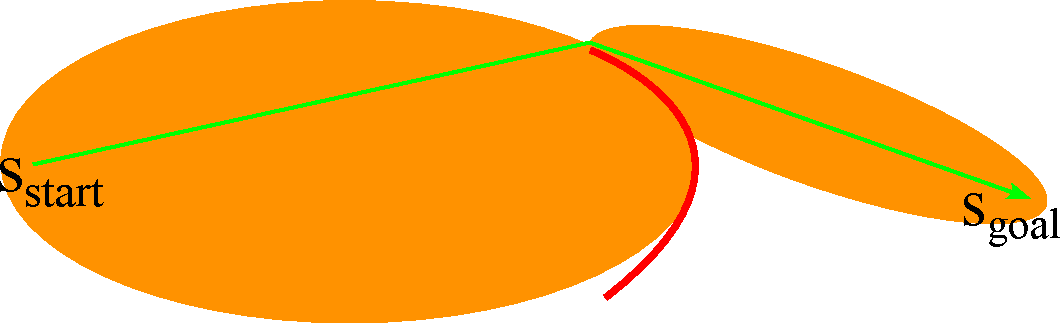
\includegraphics[width=0.8\textwidth]{doc/obrazky-figures/astar-search-space.pdf}
        \medskip
        \rule{0.8\textwidth}{0.4pt}
        \medskip
        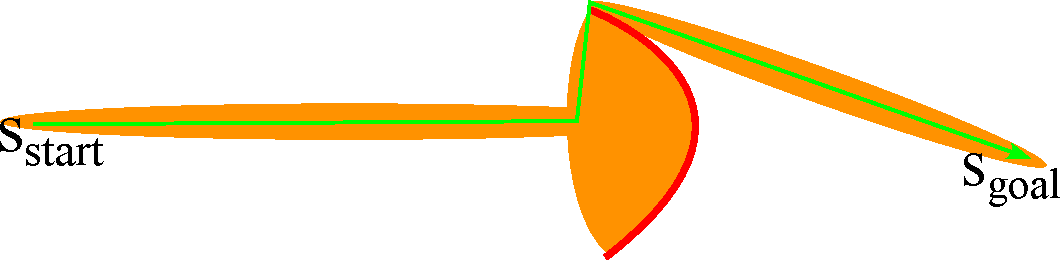
\includegraphics[width=0.8\textwidth]{doc/obrazky-figures/weighted-astar-search-space.pdf}
    \end{center}
    \caption{Porovnání prohledávaných částí stavového prostoru při použití metod \emph{A*} (nahoře) a~\emph{Weighted A*} (dole) \cite{Likachev_astar_weighted_astar}. Oranžová plocha symbolizuje prohledané stavy, zelená šipka nalezenou cestu, červená křivka překážku.}
    \label{fig:astar-wighted-astar-search-space}
\end{figure}

\subsubsection*{Metoda Anytime Repairing A*}

Myšlenka metody \emph{Anytime Repairing A*} (\emph{ARA*}) \cite{ARA_star} spočívá v~rychlém nalezení cesty, která není optimální, a~následném \uv{opravování} této cesty pro získání optimálního výsledku. Metoda opakovaně vykonává průchod stavovým prostorem metodou \emph{Weighted A*} a~při tom postupně snižuje hodnotu $\epsilon$. Hodnoty získané předcházejícími průchody si uchovává pro příští průchody, aby mohly být vykonány rychleji. Jakmile $\epsilon$ dosáhne hodnoty $1$, vykoná se poslední průchod, který již nalezne optimální řešení.

Podobně jako u~\emph{LPA*} a~\emph{D* Lite} se u~této metody hovoří o~tzv. \uv{lokální nekonzistentnosti uzlu}. Uzel $s$ je lokálně nekonzistentní, pokud existuje cesta s~cenou nižší, než je jemu aktuálně přiřazená hodnota $g(s)$.

\emph{ARA*} využívá 3 kolekce: \emph{OPEN}, \emph{CLOSED} a~\emph{INCONS}. Kolekce \emph{OPEN} je typu prioritní fronta a~plní stejnou funkci jako u~metody \emph{A*}: uchovává uzly určené k~expanzi (lokálně nekonzistentní uzly). Kolekce \emph{CLOSED} opět plní stejnou funkci jako u~metody \emph{A*}: uchovává uzly, které již expandovány byly. Na rozdíl od \emph{A*}, u~\emph{ARA*} neexistuje varianta bez kolekce \emph{CLOSED}. Kolekce \emph{INCONS} uchovává všechny lokálně nekonzistentní uzly, které již jsou v~kolekci \emph{CLOSED}. Pokud je při expanzi nějakého uzlu vygenerován uzel, který se již nachází v~kolekci \emph{CLOSED}, je umístěn do kolekce \emph{INCONS}. Na začátku jedné iterace \emph{Weighted A*} musí \emph{OPEN} obsahovat všechny lokálně nekonzistentní uzly. Při první iteraci je to počáteční uzel, při následujících iteracích je to sjednocení kolekcí \emph{OPEN} a~\emph{INCONS}.

Ukončující podmínka u~metody \emph{A*} je situace, kdy je vybrán pro expanzi cílový uzel. Jelikož však metoda \emph{ARA*} používá hodnoty získané během předchozích hledání, cílový uzel se při některém z~hledání nemusí stát lokálně nekonzistentním, a~proto se ani nedostane do kolekce \emph{OPEN}. Jiný úhel pohledu na ukončující podmínku metody \emph{A*} je, že ohodnocení $f(s_{goal})$ cílového uzlu $s_{goal}$ je nejnižší ze všech ohodnocení $f(s)$ uzlů $s$ z~kolekce \emph{OPEN}. Tohoto již je možné u~metody \emph{ARA*} dosáhnout.

\section{Metody hraní her}

Metody popsané v~této sekci se zaměřují na hry, ve kterých proti sobě soupeří dva a~více hráčů proti sobě \cite{AI_Russel_Norvig}. Výsledkem hry může být pouze stav, kdy jeden z~hráčů vyhraje a~ostatní prohrají, nebo remízový stav, kdy nelze určit vítěze ani poraženého. Hráči se postupně střídají v~tom, kdo je na tahu. Metody pro správné fungování také vyžadují, aby prostředí hry bylo deterministické a~plně pozorovatelné. Účelem těchto metod je určit, jakou akci by měl vykonat hráč na tahu.

\subsection*{Metoda Minimax}

Metodu \emph{Minimax} \cite{AI_Russel_Norvig} lze použít pouze při hře 2 hráčů. Metoda předpokládá, že oba dva hráči budou hrát optimálně, tedy že hráč na tahu se bude snažit dostat do stavu hry, který je pro něj nejvýhodnější, zatímco jeho soupeř se bude snažit dostat do stavu hry, který je nejméně výhodný pro hráče na tahu. Z~tohoto důvodu se hráč na tahu označuje jménem \emph{Max} a~jeho soupeř jménem \emph{Min}.

Podobně jako u~ostatních metod řešení úloh, i~zde se na stavový prostor hry (úlohy) nahlíží jako na vyhledávací strom, kdy kořenem je aktuální stav hry, hrany jsou akce vykonané hráčem a~listové uzly jsou konečné stavy hry, tj. výhra, prohra nebo remíza. U~většiny her by však bylo příliš náročné procházet celý stavový prostor a~hledat optimální řešení. Proto je typickou úpravou metody omezení maximální hloubky stromu. Listovým uzlem pak mohou být navíc uzly, které se nachází v~maximální hloubce.

Základem metody je funkce \emph{Minimax}, které je předán uzel $n$ a~funkce spočítá jeho ohodnocení. Hráč na tahu ji zavolá pro všechny možné stavy, do kterých se může z~aktuálního stavu dostat, a~poté vykoná akci, která vede do stavu s~nejvyšším ohodnocením. Funkce vypadá následovně:\enlargethispage{-1\baselineskip} % Keep the list items together
\begin{enumerate}
    \item Pokud je uzel $n$ listem, vrať ohodnocení tohoto uzlu.
    \item Pokud je na tahu hráč \emph{Max}, zavolej rekurzivně \emph{Minimax} pro všechny bezprostřední následníky uzlu $n$ a~vrať \emph{nejvyšší} ze získaných ohodnocení.
    \item Pokud je na tahu hráč \emph{Min}, zavolej rekurzivně \emph{Minimax} pro všechny bezprostřední následníky uzlu $n$ a~vrať \emph{nejnižší} ze získaných ohodnocení.
\end{enumerate}

Lze si všimnout, že fungování této metody se velmi podobá metodě \emph{DLS} (bez omezení hloubky stromu metodě \emph{DFS}). Obě metody expandují vždy ty uzly, které se v~rámci vyhledávacího stromu nachází nejhlouběji. Tím pádem jsou i~jejich ohodnocení podobná: pro vyhledávací strom s~faktorem větvení $b$ a~maximální hloubkou $d$ je časová složitost algoritmu $O(b^m)$ a~prostorová složitost $O(b \cdot m)$. Časovou složitost lze dále optimalizovat pomocí tzv. \emph{alfa-beta řezů}.

\subsection*{Alfa-beta řezy}

Časová složitost metody \emph{Minimax} roste exponenciálně s~rostoucí maximální hloubkou vyhledávacího stromu \cite{AI_Russel_Norvig}. Ačkoliv není možné se úplně zbavit exponentu, je možné jej snížit až na polovinu. Toho lze dosáhnout ignorováním uzlů, u~kterých víme, že na ohodnocení rodičovského uzlu nebudou mít vliv.

Příklad takových zbytečně vyšetřovaných uzlů je ukázán na obrázku~\ref{fig:alpha-beta-pruning}. Soustřeďme se na uzel označený písmenem \emph{B}. Na tahu je zde hráč \emph{Max}, tudíž hledáme nejvyšší možné ohodnocení. Při vyšetřování jeho levého podstromu bylo zjištěno, že jeho ohodnocení je 5. Při vyšetřování jeho pravého podstromu byla nalezena hodnota 4. Vzhledem k~tomu, že na tahu je v~kořeni tohoto podstromu hráč \emph{Min} a~vybírá si nejnižší možné ohodnocení, víme, že hodnota tohoto podstromu bude $\leq 4$. Tato hodnota je už nyní nižší než ohodnocení levého podstromu (5), a~tedy není nutné tento podstrom dále vyšetřovat. Ještě zajímavější je vyšetřování uzlu \emph{C}. Bylo zjištěno, že ohodnocení jeho rodiče (uzlu \emph{A}) může dosáhnout až hodnoty 6. Při vyšetřování levého podstromu uzlu \emph{C} byla vrácena hodnota 5. Jelikož je v~tomto uzlu na tahu hráč \emph{Min}, už teď víme, že jeho ohodnocení nebude vyšší než 5. V~uzlu \emph{A} je však na tahu hráč \emph{Max} a~hledá ohodnocení vyšší než 6, proto celý pravý podstrom uzlu \emph{C} může být ignorován.

\begin{figure}[ht]
    \centering
    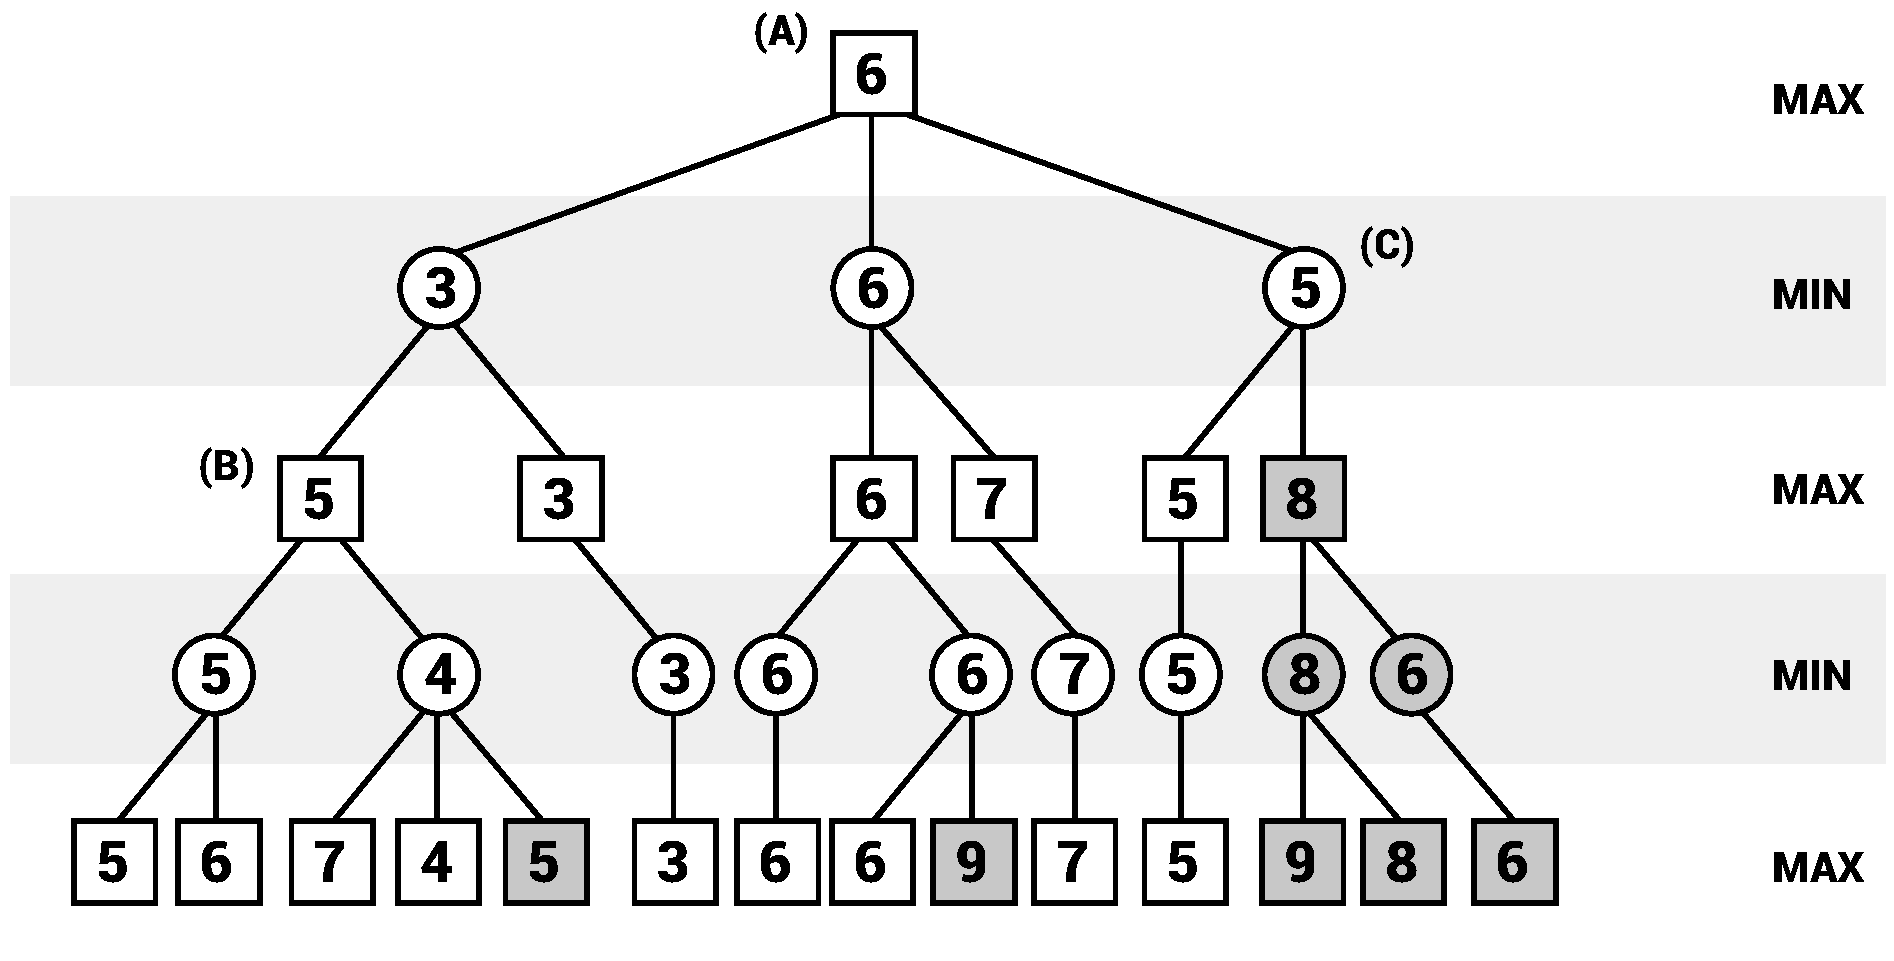
\includegraphics[width=0.8\textwidth]{doc/obrazky-figures/ab-pruning.pdf}
    \caption{Příklad vyhledávacího stromu \cite{ab_pruning} sestaveného metodou \emph{Minimax}. Čísla v~uzlech udávají jejich ohodnocení. Šedě zbarvené uzly jsou vyšetřovány zbytečně.}
    \label{fig:alpha-beta-pruning}
\end{figure}

Účelem \emph{alfa-beta řezů} je předejít tomuto zbytečnému vyšetřování uzlů. Metoda každému uzlu přiřadí proměnné $\alpha$ a~$\beta$, které se inicializují na hodnoty $-\infty$ a~$\infty$ v~tomto pořadí a~následně se modifikují před a~po rekurzivních voláních funkce \emph{Minimax}. Jakmile nastane situace $\alpha \geq \beta$, provede se \uv{řez} (\uv{alfa řez} nebo \uv{beta řez}) a~ostatní následníci uzlu, v~němž nastal tento \uv{řez} nebudou vyšetřováni. Funkce \emph{Alfa-beta} (tj. \emph{Minimax} po zavedení \emph{alfa-beta řezů}) vypadá následovně:
\begin{enumerate}
    \item Pokud je uzel $n$ listem, vrať ohodnocení tohoto uzlu.
    \item Pokud je na tahu hráč \emph{Max}, pak:
    \begin{enumerate}
        \item Dokud platí $\alpha < \beta$, volej rekurzivně funkci \emph{Alfa-beta} pro každého bezprostředního následníka uzlu $n$ s~aktuálními hodnotami $\alpha$ a~$\beta$. Pokud je vrácená hodnota \emph{vyšší} než aktuální hodnota proměnné $\alpha$, nastav hodnotu proměnné $\alpha$ na tuto vrácenou hodnotu.
        \item Pokud $\alpha \geq \beta$ (alfa řez) nebo všichni bezprostřední následníci uzlu $n$ již byli prozkoumáni, vrať aktuální hodnotu proměnné $\alpha$.
    \end{enumerate}
    \item Pokud je na tahu hráč \emph{Min}, pak:
    \begin{enumerate}
        \item Dokud platí $\alpha < \beta$, volej rekurzivně funkci \emph{Alfa-beta} pro každého bezprostředního následníka uzlu $n$ s~aktuálními hodnotami $\alpha$ a~$\beta$. Pokud je vrácená hodnota \emph{nižší} než aktuální hodnota proměnné $\beta$, nastav hodnotu proměnné $\beta$ na tuto vrácenou hodnotu.
        \item Pokud $\alpha \geq \beta$ (beta řez) nebo všichni bezprostřední následníci uzlu $n$ již byli prozkoumáni, vrať aktuální hodnotu proměnné $\beta$.
    \end{enumerate}
\end{enumerate}

Jak již bylo zmíněno, časová ani prostorová složitost se zavedením \emph{alfa-beta řezů} nezmění. V~ideálním případě je však možné snížit počet vyšetřovaných uzlů z~$b^m$ na $b^\frac{m}{2}$. Znamená to, že při použití \emph{alfa-beta řezů} můžeme prohledávat téměř $2\times$ hlubší strom než u~obyčejného \emph{Minimax} a~využít při tom stejné množství času. Onoho ideálního případu je ale velmi obtížné dosáhnout; skutečný počet vyšetřovaných uzlů se pak bude typicky pohybovat okolo hodnoty $b^{\frac{3}{4}m}$.

\subsection*{Metoda Max\textsuperscript{n}}

Metodu \emph{Minimax} nelze použít u~her, které hrají více než 2 hráči. Pro tento účel je nutné tuto metodu upravit. Tato upravená metoda bývá nazývána \emph{Max\textsuperscript{n}} \cite{Maxn}.

U~metody \emph{Minimax} pro hodnocení stavu hry stačila pouze jedna hodnota. Hráč \emph{Max} usiloval o~to, aby tato hodnota byla co největší, zatímco hráč \emph{Min} o~to, aby byla co nejmenší. U~metody \emph{Max\textsuperscript{n}} se každý hráč snaží dosáhnout hodnocení stavu hry, které je nejvýhodnější pro něj samotného. Proto místo jedné hodnoty využívá tato metoda vektor hodnot $(v_1, v_2, \ldots, v_n)$, kde $n$ je počet hráčů a~hodnota $v_i$ je ohodnocení daného stavu z~pohledu hráče $i$. Například, hrají-li hru 3 hráči a~ohodnocení stavu je dáno vektorem $(8, 2, 5)$, znamená to, že pro hráče 1 má tento stav hodnotu 8, pro hráče 2 hodnotu 2 a~pro hráče 3 hodnotu 5.

Základem metody je opět stejnojmenná funkce, \emph{maxn}, která je volána rekurzivně. Je jí předán uzel $n$, pro který funkce spočítá ohodnocení. Návratovou hodnotou je vektor ohodnocení daného uzlu, ve kterém každá hodnota přísluší právě jednomu hráči. Funkce vypadá následovně:
\begin{enumerate}
    \item Pokud je uzel $n$ listem, vrať ohodnocení tohoto uzlu.
    \item Pokud je na tahu hráč $i$, zavolej rekurzivně \emph{maxn} pro všechny bezprostřední následníky uzlu $n$ a~vrať ohodnocení, jehož $i$-tá složka je nejvyšší ze všech.
\end{enumerate}
Příklad průběhu metody je znázorněn na obrázku~\ref{fig:maxn}.

\begin{figure}[ht]
    \centering
    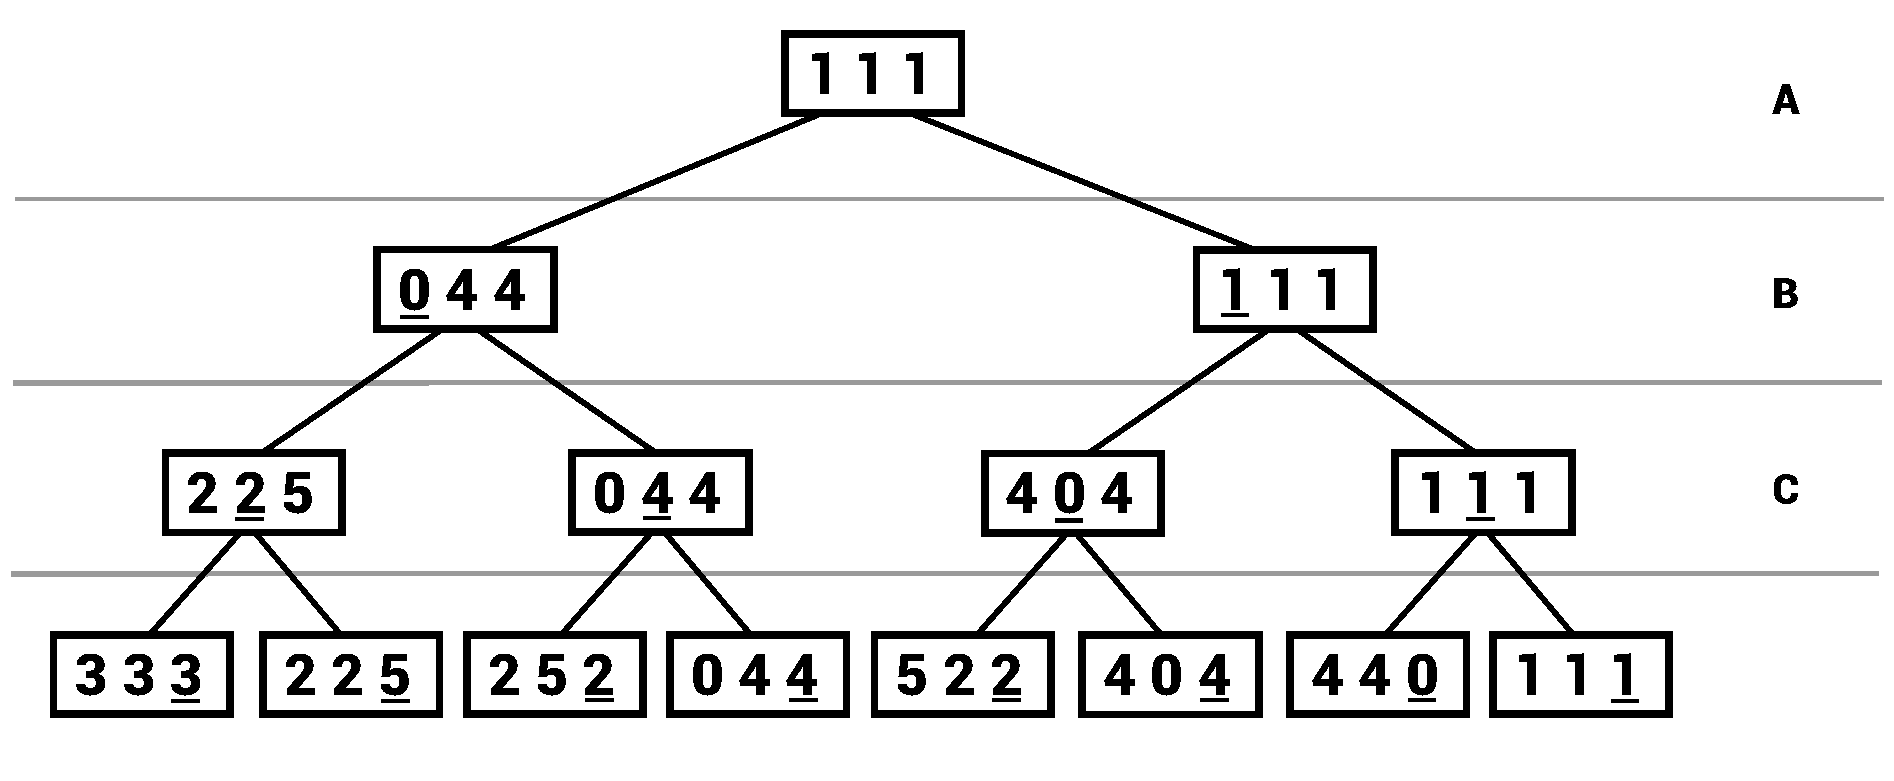
\includegraphics[width=0.8\textwidth]{doc/obrazky-figures/maxn.pdf}
    \caption{Příklad použití metody \emph{Max\textsuperscript{n}}. Čísla v~uzlech představují ohodnocení stavu pro hráče A, B a~C v~tomto pořadí. Podtržená čísla jsou ohodnocení, která jsou porovnávána při výběru nejlepšího uzlu. Příklad byl převzat z~\cite{Maxn}.}
    \label{fig:maxn}
\end{figure}

Časová složitost metody je opět exponenciální $O(b^m)$ \cite{Search_policies_in_multiplayer_games_Nijssen_Winands}. Nicméně, počet výpočtů ohodnocení stavů závisí také na počtu hráčů $n$, proto metoda bude vždy počítat okolo $nb^m$ ohodnocení stavů \cite{Maxn}. Některým těmto výpočtům lze však předejít metodou zvanou \emph{Shallow pruning}.

\subsection*{Shallow pruning}

\emph{Shallow pruning} \cite{Maxn}, stejně jako \emph{alfa-beta řezy} u~metody \emph{Minimax}, předchází nadbytečnému vyhodnocování některých hodnot metodou \emph{Max\textsuperscript{n}}. Tyto řezy bohužel nemohou ignorovat celé podstromy, jak tomu bylo u~\emph{alfa-beta řezů}, ale alespoň předchází výpočtům některých složek ohodnocení stavů.

Funkce \emph{pmaxn}, která je upravenou variantou funkce \emph{maxn}, vrací pouze jednu složku z~ohodnocení stavu a~to tu, která je použita pro porovnání v~rodičovském uzlu. Dále také vrací ukazatel na \emph{listového} potomka, kterému toto ohodnocení náleží. Pokud se vrácené ohodnocení dostane do vyšší úrovně vyhledávacího stromu, lze ukazatel na potomka využít pro vypočítání jiných složek ohodnocení stavu. Funkce vypadá takto:
\begin{enumerate}
    \item Pokud je uzel $n$ listem a~v~uzlu, který je bezprostředním předchůdcem uzlu $n$, je na tahu hráč $i$, vrať $i$-tou složku ohodnocení uzlu $n$ a~ukazatel na tento uzel.
    \item Jinak:
    \begin{enumerate}
        \item Zavolej rekurzivně \emph{pmaxn} pro každého bezprostředního následníka uzlu $n$. Najdi volání, které vrátilo nejvyšší ohodnocení, a~ulož si uzel $n^*$, kterému toto ohodnocení náleží.
        \item Pokud v~uzlu, který je bezprostředním předchůdcem uzlu $n$, je na tahu hráč $i$, vrať $i$-tou složku ohodnocení uzlu $n^*$ a~ukazatel na tento uzel.
    \end{enumerate}
\end{enumerate}

Časová složitost metody zůstává stále exponenciální $O(b^m)$, avšak skutečný počet výpočtů ohodnocení stavů je oproti \emph{Max\textsuperscript{n}} bez použití řezů nižší: přibližně
\begin{equation}
    \frac{b^{m+1} - b^{m-n+1}}{b-1}
\end{equation}
Pro odvození tohoto vztahu viz \cite{Maxn}. Účinnost metody je znázorněna na obrázku~\ref{fig:maxn-shallow-pruning}.

\begin{figure}[ht]
    \centering
    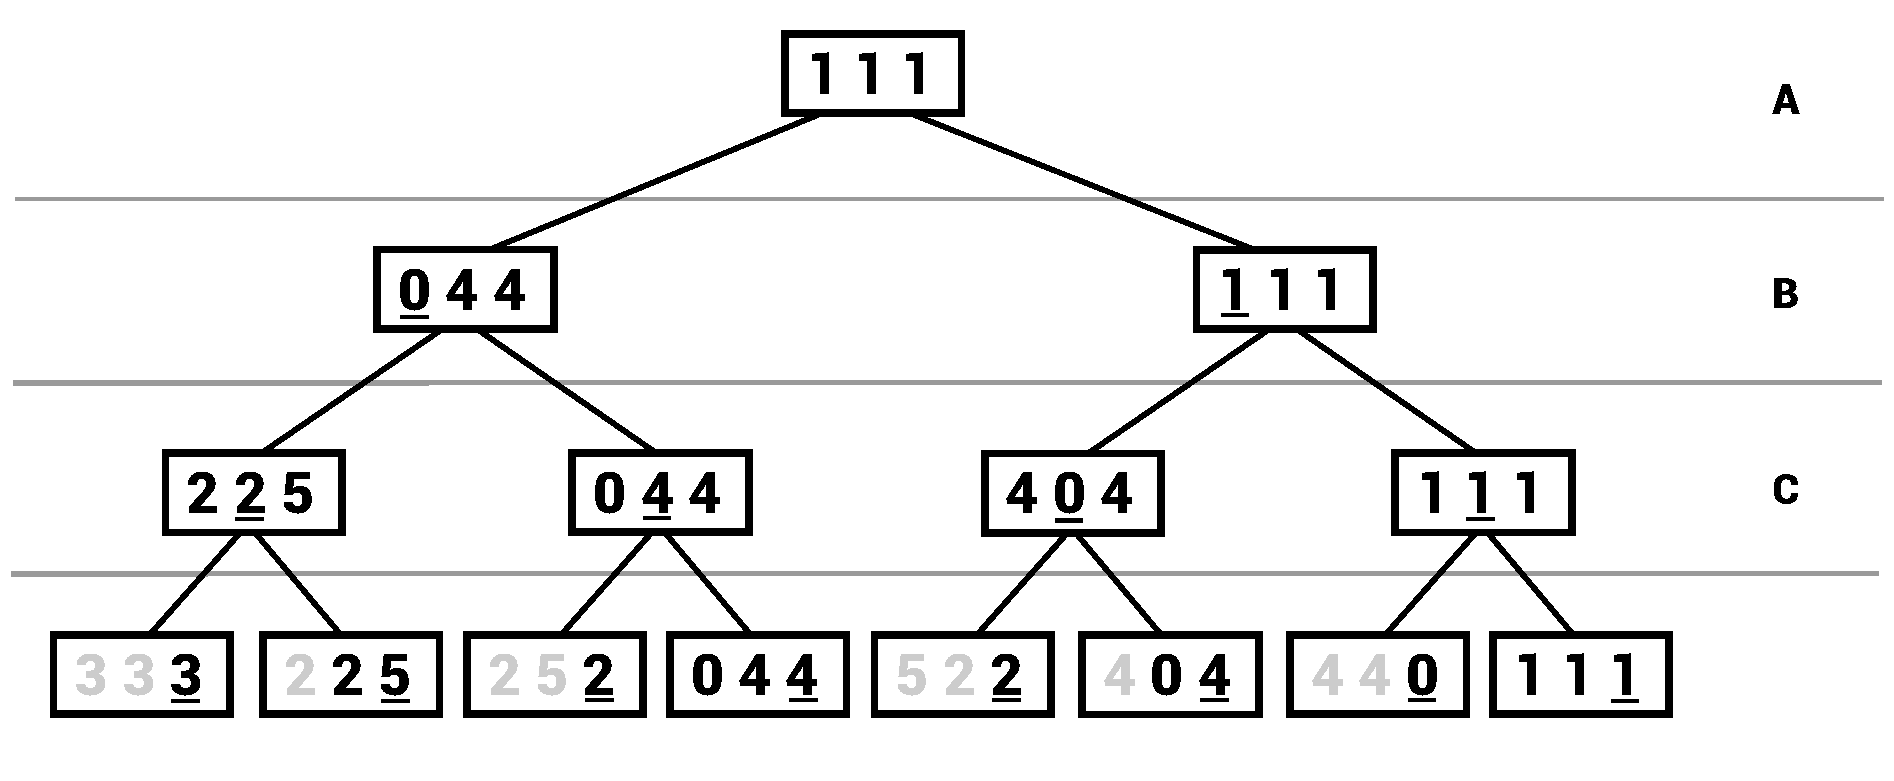
\includegraphics[width=0.8\textwidth]{doc/obrazky-figures/maxn-shallow-pruning.pdf}
    \caption{Ukázka účinnosti metody \emph{Shallow pruning} \cite{Maxn}. Stavový prostor je stejný, jako na obrázku~\ref{fig:maxn}, ale šedě zbarvená ohodnocení byla metodou \uv{ořezána}. (Ořezání je uvedeno pouze v~nejnižší vrstvě; ačkoliv metoda provádí výpočty i~ve vyšších vrstvách, jsou de facto prováděny pouze nad listovými uzly a~do vyšších vrstev se pouze propagují.)}
    \label{fig:maxn-shallow-pruning}
\end{figure}


\chapter{Představení hry}
\label{ch:predstaveni-hry}

Tato kapitola se věnuje popisu výsledné aplikace. Obsahuje popis samotné hry \emph{Bubble Brawl} a~její pravidla. Dále je zde uvedena interakce mezi uživatelem a~aplikací\,--\,ovládání, navigace mezi pohledy. Také je zde představen vestavěný editor herní plochy.

\section{Pravidla}

Hra \emph{Bubble Brawl} je typu \uv{battle royale}. Jejím cílem je tedy eliminovat všechny protivníky a~zůstat poslední naživu. Hráči ovládají kruhové entity nazývané \uv{bubliny} (\uv{bubbles}) ve 2rozměrném labyrintu. 

Hra umožňuje hráčům svislý, vodorovný i~diagonální pohyb. Překážky v~labyrintu jsou vyznačeny polygony, skrz které hráči nemohou procházet. Kromě toho představuje herní plocha obdélníkový box, který taktéž není možné opustit. Mimo pohybu je možné změnit stav bubliny tím, že hráč (manuálně) zmenší její velikost. Tato možnost existuje z~důvodu, aby bylo možné projít úzkými chodbami, pro které je bublina příliš velká. Důsledkem však je, že hráč takto ztratí body života (viz následující odstavec), nicméně nelze takto ztratit poslední bod života.

Hráči začínají s~určitým množstvím bodů života a~zůstávají ve hře, dokud je toto množství větší než 0. Když se 2 a~více hráčů dotýká, všichni dotýkající se hráči ztrácí body života. Kromě toho na této veličině závisí několik dalších vlastností hráče:
\begin{itemize}
    \item Velikost\,--\,poloměr hráčovy bubliny (přímo úměrně),
    \item Rychlost pohybu (nepřímo úměrně),
    \item Síla\,--\,kolik bodů života ubírá hráč svým protivníkům (přímo úměrně).
\end{itemize}

V~průběhu hry se v~náhodných intervalech objevují na herní ploše bonusy ve tvaru kruhu, které hráčům doplňují body života. Aby byl bonus na hráče aplikován, musí se bonus s~bublinou hráče navzájem dotýkat. Následkem toho tento bonus zmizí a~žádný jiný hráč ho poté už nemůže použít. Místo, kde se bonus objeví je náhodné. Nikdy však nemůže kolidovat s~překážkou. Navíc, v~jeden okamžik může být na herní ploše pouze jeden bonus. Množství života získané z~bonusu je také náhodně vybráno ze 4~možných hodnot relativních vůči počátečnímu množství života: $25\,\%$, $50\,\%$, $75\,\%$ a~$100\,\%$.

\section{Uživatelské rozhraní}
\label{sec:uzivatelske-rozhrani}

Aplikace se skládá z~běžných grafických komponent, jako jsou tlačítka, přepínače (\uv{\emph{radio button}}) nebo rozbalovací seznamy. Uživatel s~nimi interaguje převážně pomocí myši. Vstup z~klávesnice je použit téměř výhradně pro samotnou hru.

\subsection*{Navigace}

Po spuštění aplikace se uživateli zobrazí logo a~následně hlavní nabídka se 3 tlačítky. Tlačítko \uv{Play} zobrazí plochu pro nastavení hry. Tlačítko \emph{Stage editor} otevře editor herní plochy. Editor je popsán v~kapitole~\ref{sec:editor-herni-plochy}. Poslední tlačítko \uv{Quit} zavře aplikaci.

Uživatel musí před spuštěním hry provést nastavení hry (viz obrázek~\ref{fig:game-setup}). Nastavení sestává z~výběru herní plochy, na níž se bude hra hrát, určení počtu hráčů a~jejich typů.

\begin{figure}[ht]
    \centering
    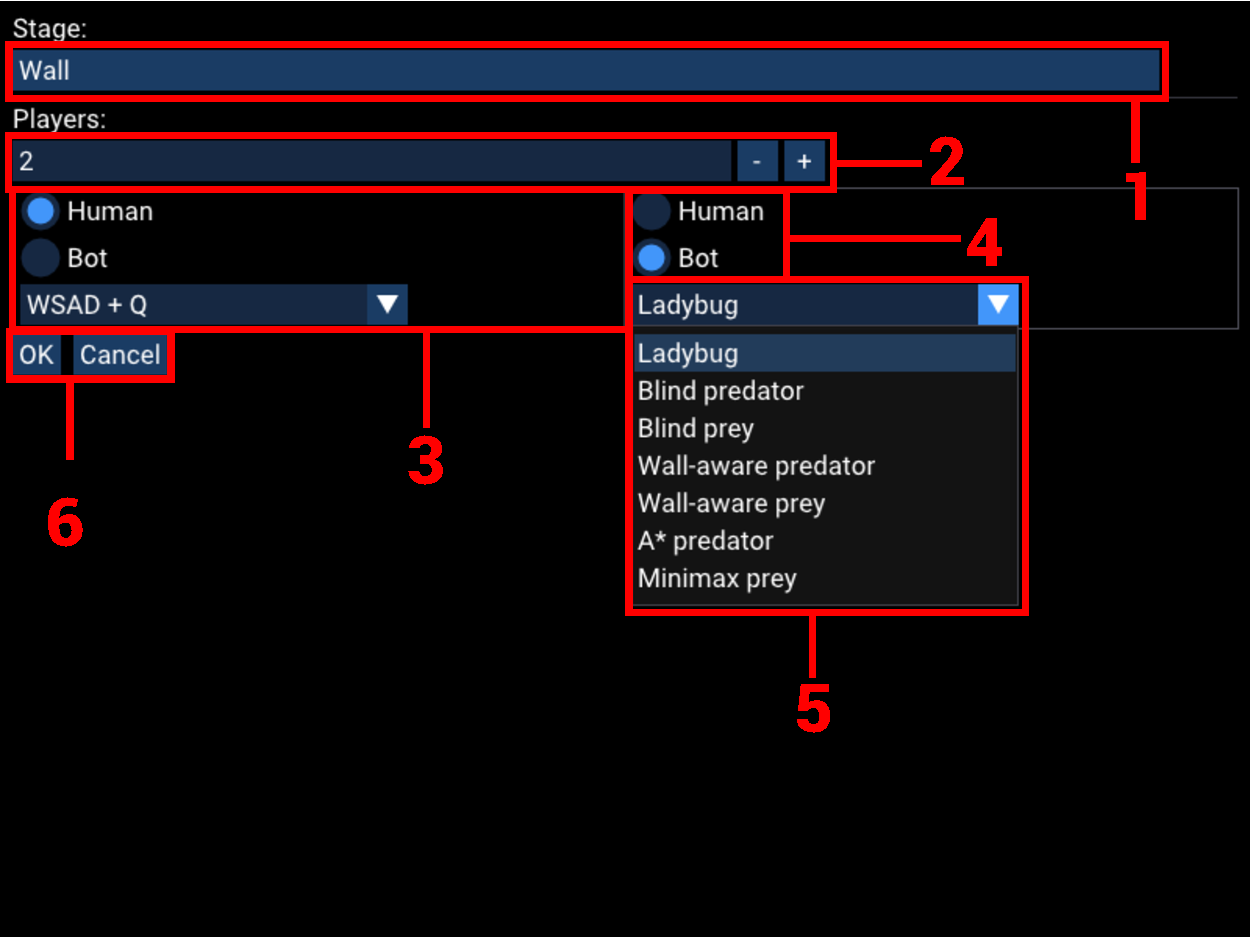
\includegraphics[width=0.8\textwidth]{doc/obrazky-figures/game-setup.pdf}
    \caption{Plocha pro nastavení hry. Tlačítko (1) umožňuje výběr herní plochy. Textové pole (2) umožňuje nastavit počet hráčů. Panel (3) seskupuje nastavení týkající se konkrétního hráče a~obsahuje přepínače (4) pro výběr typu hráče a~rozbalovací seznam (5) pro výběr ovládání hráče. Pomocí tlačítek (6) lze spustit hru nebo vrátit se zpět na hlavní nabídku.}
    \label{fig:game-setup}
\end{figure}

Po kliknutí na tlačítko označené popiskem \uv{Stage:} se zobrazí seznam existujících herních ploch. Uživatel zde může vybrat nějakou položku ze seznamu nebo se tlačítkem \uv{Cancel} vrátit zpět na plaochu nastavení hry bez výběru herní plochy.

Pokud je nějaká herní plocha vybrána, může uživatel nastavit počet hráčů ve hře pomocí textového pole \uv{Players:}. Maximální hodnota tohoto pole je rovna maximálnímu počtu hráčů, který na vybrané herní ploše může hrát.

S~měnící se hodnotou v~tomto poli se také mění počet panelů pro nastavení jednotlivých hráčů. V~těchto panelech se nachází přepínače, kde hráč může vybrat typ hráče: člověk (\uv{Human}) nebo počítač (\uv{Bot}). Na základě vybraného typu hráče se mění funkce rozbalovacího seznamu: pokud uživatel vybral přepínač \uv{Human}, rozbalovací seznam slouží pro výběr kláves, pomocí kterých bude hráč ovládat svoji \uv{bublinu}. Pokud uživatel vybral přepínač \uv{Bot}, pak rozbalovací seznam bude obsahovat různé typy těchto \uv{botů}. Umělé inteligenci se věnuje kapitola~\ref{sec:entity-rizene-pocitacem}. Zde se pouze zmíním o~tom, že typ \uv{Ladybug} se pohybuje čistě náhodně, typ \uv{Predator} se snaží vždy útočit a~\uv{Prey} se snaží vždy utíkat.

Pokud bylo vše vyplněno správně, je možné tlačítkem \uv{OK} spustit hru. V~opačném případě bude tlačítko zašedlé a~nepůjde na něj kliknout. Aby bylo možné spustit hru, musí být vybrána herní plocha a~nesmí být 2 různí hráči typu \uv{Human}, kteří jsou ovládáni stejnými klávesami. Není však problém, pokud počet hráčů je 0 nebo 1; v~tomto případě hra ihned po spuštění skončí. Z~plochy nastavení hry je možné se kdykoliv vrátit zpět na hlavní nabídku pomocí tlačítka \uv{Cancel}.

\subsection*{Probíhající hra}

Plocha, na níž je zobrazen aktuální stav hry, je rozdělena na 2 části: herní plochu a~boční panel (viz obrázek~\ref{fig:in-game}). Herní plocha zobrazuje aktuální stav hry\,--\,hráče, překážky a~bonusy. Hráči jsou na herní ploše vyznačeni pomocí barevných kruhů, přičemž každému hráči patří jiná barva. Překážky včetně ohraničení herní plochy jsou znázorněny šedými polygony. Bonusy jsou světle modré kruhy s~červeným ohraničením a~červeným symbolem \uv{plus} uprostřed. Po sebrání se bonus změní na text informující o~tom, jaké množství života hráč z~bonusu získal.

\begin{figure}[ht]
    \centering
    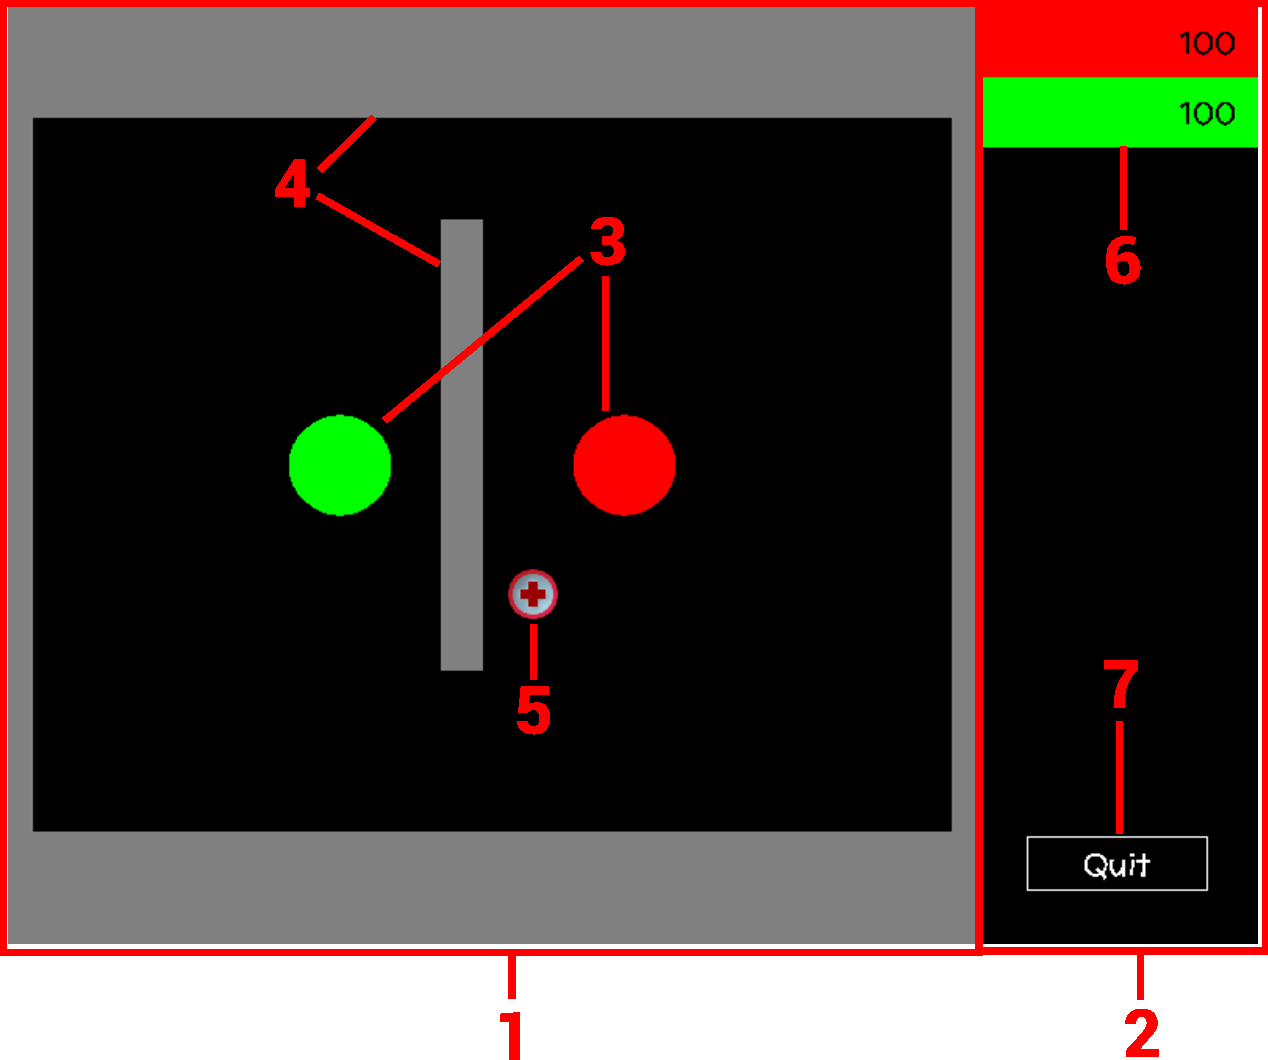
\includegraphics[width=0.8\textwidth]{doc/obrazky-figures/in-game.pdf}
    \caption{Plocha s~probíhající hrou. Plocha je rozdělena na herní plochu (1) a~boční panel (2). Na herní ploše se zobrazují herní objekty\,--\,hráči (3), překážky (4) a~bonusy (5). V~bočním panelu se nachází počítadla množství života hráčů (6) a~tlačítko pro ukončení hry (7).}
    \label{fig:in-game}
\end{figure}

Boční panel je umístěn vpravo. V~jeho horní části se nachází počítadla množství života hráčů, jejichž barvy odpovídají barvám hráčů. Jakmile je nějaký hráč vyřazen ze hry, jeho počítadlo je skryto. Hru je možné kdykoliv ukončit tlačítkem \uv{Quit} v~dolní části bočního panelu.

Jakmile zůstal ve hře pouze 1 hráč, zobrazí se uprostřed herní plochy nápis \uv{WINNER} (\uv{vítěz}). Pokud nastane situace, že na herní ploše není ani jeden hráč, zobrazí se místo toho nápis \uv{DRAW GAME} (\uv{remíza}). Hra i~potom pokračuje dál; bonusy se na herní ploše dále objevují a~hráč, pokud je nějaký naživu, se může po herní ploše volně pohybovat.

\section{Editor herní plochy}
\label{sec:editor-herni-plochy}

Uživatel má možnost vytvářet vlastní herní plochy pomocí vestavěného editoru. Editor lze spustit z~hlavního menu tlačítkem \uv{Stage editor}.

Editor herní plochy se skládá z~menu, panelu nástrojů a~pracovní plochy, viz obrázek~\ref{fig:stage-editor}. V~menu se nachází tlačítka pro načítání a~ukládání herní plochy, dále tlačítka pro krok zpět a~vpřed (\uv{Undo} a~\uv{Redo}) a~vpravo tlačítko pro návrat do hlavního menu. Panel nástrojů obsahuje nástroje, které slouží pro manipulaci s~objekty na herní ploše. Pracovní plocha slouží pro samotné sestavování herní plochy.

\begin{figure}[ht]
    \centering
    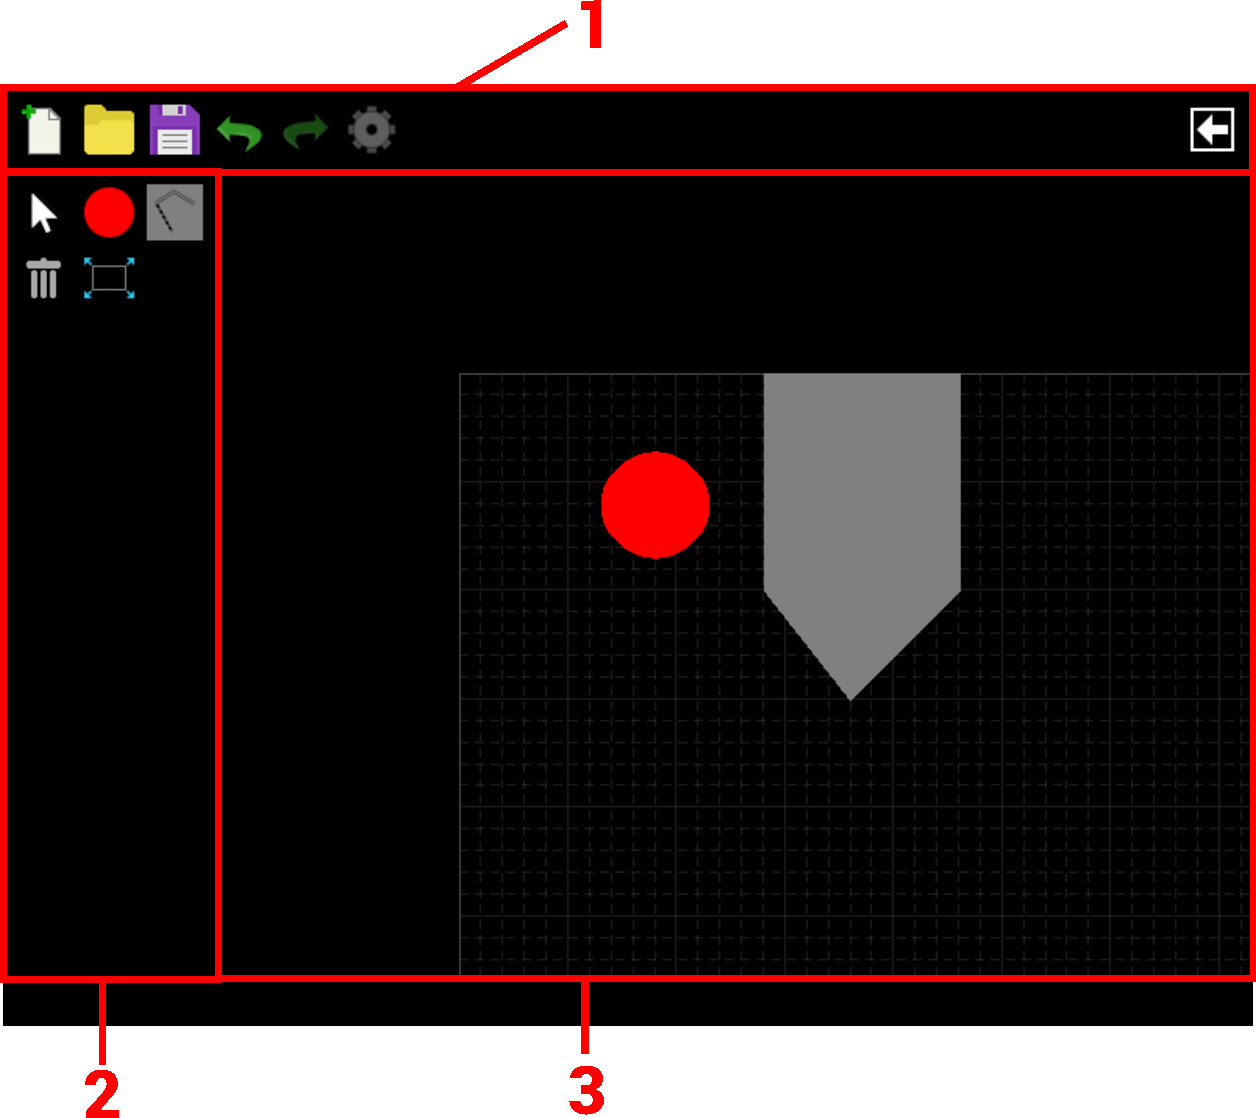
\includegraphics[width=0.8\textwidth]{doc/obrazky-figures/stage-editor.pdf}
    \caption{Editor herní plochy. Skládá se z~menu (1), panelu nástrojů (2) a~pracovní plochy (3).}
    \label{fig:stage-editor}
\end{figure}

% Describe editor button
% Parameters:
%  #1 Button name
%  #2 Path to button image
%  #3 Button description
\newcommand{\describeeditorbutton}[3]{
\noindent\begin{tabularx}{\textwidth}{lX}
    \scalebox{2}{\includegraphics[valign=b]{#2}} & \textbf{#1}\,--\,#3 \\
    \\
\end{tabularx}
}

Následují vysvětlivky jednotlivých tlačítek. Obrázky tlačítek byly převzaty přímo z~výsledné aplikace.\\

\describeeditorbutton{New}{doc/obrazky-figures/new.png}{Vytvoří novou, prázdnou herní plochu.}

\describeeditorbutton{Open}{doc/obrazky-figures/open.png}{Zobrazí seznam existujících herních ploch. Po kliknutí na některou z~položek tohoto seznamu nahraje vybranou herní plochu ze souboru.}

\describeeditorbutton{Save}{doc/obrazky-figures/save.png}{Uloží rozpracovanou herní plochu do souboru. Pokud k této ploše není přiřazen žádný soubor (nebyla načtena ze souboru a ani zatím nebyla ukládána), vytvoří se nový soubor. Jeho název bude vybrán podle pravidel popsaných níže.}

\describeeditorbutton{Undo}{doc/obrazky-figures/undo.png}{Vrátí se zpět do stavu před poslední vykonanou akcí. Opakovaným stiskem tohoto tlačítka se lze vrátit do stavu před vykonáním více než jedné akce.}

\describeeditorbutton{Redo}{doc/obrazky-figures/redo.png}{Opakuje poslední akci vrácenou pomocí tlačítka \uv{Undo}. Pokud zatím nebylo provedeno \uv{undo}, nebo od jeho posledního vykonání byla provedena jiná akce, nestane se nic. Opakovaným stiskem tohoto tlačítka lze opakovat více než jednu vrácenou akci.}

\describeeditorbutton{Stage properties}{doc/obrazky-figures/cogwheel.png}{Umožňuje změnit vlastnosti týkající se herní plochy. Zobrazí se okno s~textovou kolonkou, kde má uživatel možnost změnit název herní plochy. Pod kolonkou je zobrazen název souboru, do kterého bude herní plocha uložena při dalším stisku tlačítka \uv{Save}.}

\describeeditorbutton{Select tool}{doc/obrazky-figures/select-tool.png}{Umožňuje přesouvat a~upravovat již existující objekty na herní ploše. Objekt je nejdříve nutné vybrat kliknutím. Lze také vybrat více objektů přidržením klávesy \texttt{Shift} a~následně přesunout všechny vybrané objekty najednou. Při přesouvání je nutné dodržovat pravidla uvedená u~jednotlivých nástrojů pro objekty níže, jinak nebude přesun proveden.}

\describeeditorbutton{Player tool}{doc/obrazky-figures/player-tool.png}{Umožňuje přidávat na herní plochu objekty hráčů. Přidané objekty nesmí kolidovat s~objekty překážek, jiných hráčů, ani nesmí zasahovat mimo hranice herní plochy, jinak nebude objekt na herní plochu přidán. Pokud je vybrán tento nástroj, zobrazí se na pozici kurzoru myši bílá přerušovaná kružnice. Není-li možné na danou pozici objekt hráče umístit, kružnice zčervená.}

\describeeditorbutton{Obstacle tool}{doc/obrazky-figures/obstacle-tool.png}{Umožňuje konstruovat objekty překážek na herní ploše. Konstrukce překážky probíhá přidáváním jednotlivých vrcholů na herní plochu a~následným uzavřením objektu stiskem pravého tlačítka myši. Nově přidané hrany se nesmí překrývat s~existujícími hranami konstruovaného objektu, ani s~objekty hráčů. Nicméně, dvě a~více překážek se smí překrývat. Pokud byl na pracovní plochu umístěn alespoň jeden vrchol a~překážka zatím nebyla uzavřena, zobrazí se mezi všemi propojenými body plná šedá čára a~mezi posledním bodem a~kurzorem myši čára přerušovaná. Není-li možné na danou pozici umístit vrchol, přerušovaná čára zčervená. Změna aktivního nástroje během konstruování překážky způsobí přerušení konstruování.}

\describeeditorbutton{Delete tool}{doc/obrazky-figures/trash-can.png}{Umožňuje mazat objekty na herní ploše. Pokud byly nějaké objekty vybrány pomocí nástroje \uv{Select tool}, pak při kliknutí na některý z~vybraných objektů budou odstraněny všechny vybrané objekty. Pokud není vybrán žádný objekt, odstraní se pouze ten, na který uživatel klikl.}

\describeeditorbutton{Resize stage tool}{doc/obrazky-figures/resize.png}{Umožňuje měnit velikost herní plochy přetažením jejího pravého dolního rohu. Při změně velikosti nesmí dojít k~tomu, aby některý z~hráčů zasahoval mimo hranice herní plochy, jinak nebude změna provedena.}

Uživatel nemá možnost vybírat si název souboru s~herní plochou. Soubory jsou vždy ukládány do adresáře \uv{\texttt{stage/}}. Pokud nebyla herní plocha načtena ze souboru, název souboru je vygenerován podle názvu herní plochy tímto způsobem:
\begin{enumerate}
    \item Všechna velká písmena se změní na malá. Všechny mezery se změní na podtržítka.
    \item Vyjmou se všechny nealfanumerické znaky, které nejsou podtržítka.
    \item Pokud název přesahuje 28 znaků, přebývající znaky na konci řetězce se odstraní.
    \item Pokud je název prázdný řetězec, použije se výchozí \uv{stage}.
    \item Pokud již v~adresáři \texttt{stage/} existuje soubor se stejným názvem, připojí se na konec názvu souboru číslo \uv{1}. Pokud i~tento soubor již existuje, číslo se zvyšuje do té doby, než je nalezen unikátní název.
\end{enumerate}
Soubor je následně možné manuálně přejmenovat; tedy není nutné, aby název souboru a~herní plochy navzájem dodržovaly výše zmíněná pravidla.

Pracovní plochu lze přiblížit nebo oddálit přidržením klávesy \texttt{Ctrl} a~otáčením kolečka myši. Lze se také po ní posouvat pohybem myši za přidržení jejího kolečka.

Uvnitř herní plochy se zobrazuje mřížka přerušovaných čar, která pomáhá s~umísťováním objektů. Mřížka má různé úrovně hustoty dle přiblížení herní plochy. Při konstrukci objektů jsou body přichytávány k~průsečíkům čar. Tuto funkci je možné deaktivovat přidržením klávesy \texttt{Alt}, což zaručí, že jednotlivé body se budou přichytávat pouze ke kurzoru myši.

\subsection*{Pravidla pro výchozí pozice hráčů}

Pravidla pro výchozí pozice hráčů je prvek aplikace, který byl původně součástí návrhu, avšak do výsledné aplikace se nedostal, neboť se jej nepovedlo implementovat. Ačkoliv je součástí souborů s~herní plochou (viz níže), editor herní plochy neumožňuje tuto informaci upravovat a~samotné jádro hry tuto informaci ignoruje. Přesto je zde popsán, aby bylo v~budoucnu možné se pokusit o~jeho implementaci.

Pravidla pro výchozí pozice hráčů určují pozice, na které budou hráči umístěni na začátku hry. Pravidel může být několik. Při spuštění hry se pak dle počtu hráčů vybere z~vyhovujících pravidel to nejvíce omezující. Příklad: k~dispozici jsou možnosti pro 2 nebo 4 hráče, hru budou hrát 3 hráči. Vybere se tedy pravidlo pro 4 hráče a~využijí se pozice prvních 3 hráčů. Tímto je navíc určen maximální počet hráčů pro danou plochu\,--\,zde 4.

\subsection*{Ukládání vytvořené herní plochy}

Uživatelem vytvořené herní plochy přetrvávají po ukončení programu. Uloženy jsou v~souborech typu YAML\footnote{Viz oficiální web: \url{https://yaml.org/}}. O~herních plochách se uchovávají tyto informace:

\begin{itemize}
    \item název (\texttt{title}),
    \item šířka (\texttt{width}),
    \item výška (\texttt{height}),
    \item hráči (\texttt{players}),
    \item překážky (\texttt{obstacles}),
    \item pravidla pro výchozí pozice hráčů (\texttt{positionRules}).
\end{itemize}

Název je uložen ve formě řetězce a~může obsahovat libovolné Unicode znaky. Šířka a výška jsou celá kladná čísla.

Hráči jsou uloženi ve formě seznamu uspořádaných dvojic reálných čísel, kde první hodnota představuje souřadnici X středu hráčovy \uv{bubliny} a~druhá souřadnici Y. Velikost (poloměr) hráče se neukládá; je vždy přesně 50.

Překážky jsou popsány kolekcí trojúhelníků. Překážky, které mají více než tři vrcholy, musí program rozdělit na trojúhelníky. Hlavním důvodem je, aby se předešlo \uv{sebeprotínání}\footnote{Hranice polygonů, které mají více než 3 hrany, mohou protínat samy sebe. Trojúhelníků se tento problém netýká.}. Editor herní plochy sice pracuje s~polygony, ale nedovolí vytvořit polygon, v~němž se protínají hrany.

Pravidla pro výchozí pozice hráčů jsou uložena ve formě pole indexů do seznamu hráčů.

Níže je uveden příklad souboru YAML popisujícího herní plochu. Uprostřed plochy se nachází překážka tvaru obdélníku. Výchozí pozice hráčů jsou v rozích herní plochy. Při hře dvou hráčů jsou výchozí pozice nastaveny na protilehlé rohy:
\begin{center}
\begin{minipage}{\textwidth}
    \begin{verbatim}
---
stage:
    title: My stage
    width:  1920
    height: 1080
    players: 
        - [50, 50]
        - [1870, 50]
        - [50, 1030]
        - [1870, 1030]
    obstacles:
        - [[720, 405], [720, 675], [1200, 675]]
        - [[1200, 675], [1200, 405], [720, 405]]
    positionRules:
        - [0, 1, 2, 3]
        - [0, 3]
    \end{verbatim}
\end{minipage}
\end{center}


\chapter{Implementace}
\label{ch:implementace}

V~této kapitole jsou popsány důležité části implementace aplikace. Kód aplikace je psán v jazyce \emph{C++}, standard \emph{C++20}, a~skripty pro překlad a~sestavení jsou v jazyce \emph{CMake}. Při vývoji byl použit verzovací nástroj \emph{Git} a~samotný repozitář projektu je veřejně dostupný na platformě \emph{GitHub}\footnote{\url{https://github.com/T0mmiTheGreat/bc-thesis}}.


\section{Použité knihovny}

\subsection*{Simple DirectMedia Layer}

\emph{SDL}\footnote{\url{https://www.libsdl.org/}} (\emph{Simple DirectMedia Layer}) je multiplatformní knihovna, která poskytuje nízkoúrovňový přístup ke vstupu z~klávesnice, myši, joysticku, výstupu zvuku a~grafiky. Je napsána v~jazyce \emph{C} a~funguje nativně i~v~jazyce \emph{C++}. Oficiálně podporuje platformy Windows, macOS, Linux, Android a~iOS. V~projektu je použita verze~2 této knihovny (\emph{SDL2}), která byla v~době psaní práce nejnovější stabilní verzí.

Knihovna \emph{SDL} umožňuje vykreslovat 2D i~3D grafiku. Využívá akcelerovaná API, jako například \emph{OpenGL} nebo \emph{Direct3D}. Běžné je také použití \emph{SDL} v~kombinaci s~knihovnou \emph{OpenGL}, kdy \emph{OpenGL} je využito pro větší akceleraci vykreslování a~\emph{SDL} pro vše ostatní\,--\,vytváření oken, uživatelský vstup, audio apod.

\emph{SDL} má také několik přidružených knihoven, které rozšiřují její funkcionalitu. V~projektu jsou použity knihovny \emph{SDL\_Image} a~\emph{SDL\_TTF}.

\emph{SDL\_Image} slouží pro načítání obrázků ze souborů. Knihovna podporuje množství běžně používaných grafických formátů, jako například PNG, JPEG, BMP, GIF, SVG a~jiné.

\emph{SDL\_TTF} se stará o~načítání písem ze souborů a~vykreslování textu. Jedná se v~posdtatě o~\uv{wrapper} pro knihovny \emph{Freetype} a~\emph{Harfbuzz} s~tím, že výsledkem vykreslování je objekt \texttt{SDL\_Surface}, který je následně možné použít v~rámci \emph{SDL}.

Všechny tři knihovny jsou distribuovány pod licencí \emph{zlib}.

\subsection*{libSDL2pp}

Knihovna \emph{libSDL2pp}\footnote{\url{https://sdl2pp.amdmi3.ru/}} slouží pro zastoupení knihovny \emph{SDL2} a~přidružených knihoven pomocí objektového modelu jazyka \emph{C++}. Důležitým prvkem knihovny je zabalení objektů knihovny \emph{SDL} do objektů jazyka \emph{C++}, což umožňuje jejich správu technikou \emph{RAII}. Dále je užitečné také využití výjimek místo návratových kódů pro hlášení chyb, nebo přetížení některých funkcí a~metod.

\emph{libSDL2pp} není kompletní; existuje řada funkcí z~knihovny \emph{SDL}, které v~\emph{libSDL2pp} nemají ekvivalent a~je nutné volat přímo ty z~\emph{SDL}. Jedná se většinou o~ty, které nemohou skončit chybou a~není tedy nutné pro ně ekvivalent v~této knihovně vytvářet. Knihovna se vyvíjí především dle potřeb jejího autora. Nicméně, do veřejného repozitáře této knihovny na platformě \emph{GitHub} přispívá i~spousta jiných vývojářů. Knihovna je distribuována pod licencí \emph{zlib}.

\subsection*{SDL\_gfx}

Knihovna \emph{SDL\_gfx}\footnote{\url{https://www.ferzkopp.net/wordpress/2016/01/02/sdl_gfx-sdl2_gfx/}} slouží pro vykreslení některých základních geometrických tvarů, které \emph{SDL} v~základu nepodporuje, jako jsou například křivky a~elipsy. Je napsána v~jazyce \emph{C} a~funguje nativně i~v~\emph{C++}.

Samotná knihovna \emph{SDL} dokáže vykreslovat úsečky, body, mnohoúhelníky a textury. Specializované funkce pro kreslení elips nebo křivek v~\emph{SDL} chybí. \emph{SDL\_gfx} implementuje tyto chybějící funkce s~použitím funkcí, které \emph{SDL} poskytuje.

Knihovna je distribuována pod licencí \emph{zlib}.

\subsection*{Dear ImGui}

\emph{Dear ImGui}\footnote{\url{https://github.com/ocornut/imgui}} je knihovna pro tvorbu grafických uživatelských rozhraní v~jazyce \emph{C++}. Je rychlá, přenositelná a~nevyžaduje žádné další knihovny.

Účelem knihovny je především umožnit vytváření nástrojů pro tvorbu obsahu, vizualizaci nebo ladění, a~nezaměřuje se přímo na tvorbu kompletních uživatelských rozhraní. Proto postrádá některé prvky, které se běžně vyskytují v~knihovnách pro tvorbu uživatelských rozhraní (jako například rozšířené možnosti rozmisťování komponent).

Zdrojové soubory jsou rozděleny na několik souborů nezávislých na platformě, na které běží, a~jednotlivé \emph{backendy}, které se starají o~integraci knihovny s~grafickým a~vstupně-výstupním API. Díky tomuto rozdělení umožňuje relativně jednoduché vytváření rozšíření pro další digitální platformy. Nicméně, sama knihovna v~současné době poskytuje \emph{backendy} pro renderování pomocí \emph{DirectX}, \emph{Metal}, \emph{OpenGL}, \emph{SDL\_renderer}, \emph{Vulkan} a~\emph{WebGPU}, platformy \emph{GLFW}, \emph{SDL}, \emph{Win32}, \emph{Glut}, \emph{OSX} a~\emph{Android} a~frameworky \emph{Allegro5} a~\emph{Emscripten}.

Knihovna je distribuována pod licencí \emph{MIT license}.

\subsection*{Computational Geometry Algorithms Library}

\emph{Computational Geometry Algorithms Library}\footnote{\url{https://www.cgal.org/}} (\emph{CGAL}) je knihovna pro jazyk \emph{C++}, která poskytuje efektivní a~spolehlivé algoritmy z~oblasti výpočetní geometrie. Využívána je v~mnoha oblastech vyžadujících geometrické výpočty, mezi které patří například geografické informační systémy (\emph{GIS}), počítačem podporované projektování (\emph{CAD}), molekulární biologie, zobrazovací metody v~lékařství, počítačová grafika, nebo robotika.

Knihovna poskytuje rozsáhlé množství struktur a~algoritmů. Kromě základních n-roz\-měr\-ných geometrických útvarů a~operací nad nimi nabízí knihovna také triangulace, polygonové sítě, konvexní obaly, Voroného diagramy a~spoustu dalších.

\emph{CGAL} je založena na \uv{\emph{exact computation paradigm}}, díky čemuž dokáže při správném použití vracet vždy správné výsledky. Je to díky tomu, že nepoužívá číselné typy s~omezenou přesností (pokud to volající přímo nevyžaduje), ale místo toho počítá s~čísly s~libovolnou přesností. Ovšem cenou za přesnost je doba výpočtu.

Knihovna používá duální licencování. Je dostupná pod otevřenou (\emph{open source}) licencí, kde některé části knihovny jsou distribuovány s~licencí \emph{LGPL} a~jiné s~\emph{GPL}. Pokud však uživateli nevyhovují omezení plynoucí z~otevřené licence, je možné si \emph{CGAL} zakoupit pod komerční licencí.

\subsection*{yaml-cpp}

\emph{yaml-cpp}\footnote{\url{https://github.com/jbeder/yaml-cpp}} je otevřená (\emph{open source}) knihovna pro jazyk \emph{C++}, která umožňuje číst a~vytvářet data serializovaná pomocí jazyka \emph{YAML}.

\emph{yaml-cpp} dokáže načíst a~zpracovat data ve formátu \emph{YAML} ze souboru nebo z~řetězce. Výsledkem zpracování dat knihovnou je stromová struktura uzlů různých datových typů. Výsledný strom je následně možné dále modifikovat připojováním, odstraňováním nebo přepisováním uzlů. Při čtení je následně možné převádět jak listové uzly do nativních datových typů (\texttt{int}, \texttt{double}, \texttt{std::string} aj.), tak celé podstromy do strukturovaných datových typů (\texttt{std::vector}, \texttt{std::list} a~\texttt{std::map}). Knihovna také umožňuje vytvářet vlastní konverze pro jiné datové typy (vestavěné i~uživatelem definované).

Generování \emph{YAML} probíhá v~\emph{yaml-cpp} podobným způsobem jako zapisování do \emph{streamů} v~jazyce \emph{C++}\,--\,hodnoty se zapisují do \uv{\emph{emitoru YAML}} použitím operátoru \uv{\texttt{<{}<}}. \emph{Emitor} dokáže zpracovat literály (číselné, řetězcové) i~struktury (\texttt{std::vector}, \texttt{std::list} a~\texttt{std::map}). Stejně jako při čtení \emph{YAML}, lze i~pro generování definovat vlastní pravidla pro jiné datové typy.

Knihovna je distribuována pod licencí \emph{MIT license}.


\section{Architektura programu}

Program je postaven na architektonickém vzoru \emph{Model-View-Controller} (\emph{MVC}) s~drobným rozdílem: mezi vrstvami \emph{View} a~\emph{Model} je pouze tenká vazba. Data z~vrstvy \emph{Model} nejsou zobrazována přímo, ale jsou předávána skrze vrstvu \emph{Controller}. Tato vrstva rozhodne o~tom, jakým způsobem budou data z~\emph{Modelu} interpretována a~\emph{View} následně dle této interpretace určí, jakým způsobem je zobrazí. Stejně jako u~\emph{MVC}, \emph{Controller} je hlavní komponentou programu a~řídí jeho tok\,--\,přijímá události, jako napříkald stisk klávesy či pohyb myši, a~předává je vrstvě \emph{Model} a~také se stará o~změny hodnot atributů ve \emph{View}.

Vrstva \emph{View} je zastoupena třídami implementujícími rozhraní \texttt{ISprite}. Jsou to v~podstatě dvourozměrné obrázky nacházející se na daných souřadnicích na obrazovce. Kromě pozice mají konkrétní \emph{sprity} další atributy, jako například (v~případě hráče) barva, velikost, nebo (v~případě tlačítka v~menu) \emph{kostým}\footnote{Pojmenování \uv{kostým} bylo převzato z programovacího jazyka \emph{Scratch}: \url{https://scratch.mit.edu/}.}, což je pojmenovaný vzhled \emph{spritu}.

Vrstva \emph{Controller} je zastoupena třídami označovanými jako \texttt{Controller}. Jsou 2 druhy této třídy s~různými rozhraními: \texttt{RootController} a \texttt{ChildController}. \texttt{Root\-Con\-trol\-ler} je pouze jeden; uchovává právě aktivní \texttt{ChildController} a~přeposílá mu události. Tříd druhu \texttt{ChildController} je několik a~představují různé části aplikace. Například, existuje jeden pro hlavní menu, jiný pro probíhající hru, jiný pro editor herní plochy apod. Jelikož je vrstva \emph{Controller} ústřední součástí architektury programu, třídy \texttt{ChildController} vytváří, uchovávají a~nakonec také odstraňují třídy představující \emph{View} a~\emph{Model}. Dále také vybírají \texttt{ChildController}y, které je v~\texttt{RootController}u mají nahradit; například, hlavní menu při stisku tlačítka vytvoří a~\texttt{RootController}u předá \texttt{ChildController} pro editor herní plochy.

Třídy zastupující vrstvu \emph{Model} vzoru \emph{MVC} mají různá pojmenování a~nemají jednotné rozhraní. Vztahují se vždy přímo k~jedné třídě \texttt{Controller}, avšak ne každá třída \texttt{Controller} má svoji třídu z~vrstvy \emph{Model}. Například hlavní menu slouží pouze pro navigaci, kterou je vhodné řešit na vrstvě \emph{Controller}, a~tudíž nemá žádný \emph{Model}.


\section{Přenositelnost}

Program byl psán s~cílem, aby byl co nejvíce přenositelný na různé platformy. Samotný programovací jazyk \emph{C++} je přeložitelný na spoustě různých platforem a~dokonce i~vestavěných systémů. Volba knihovny \emph{SDL} limituje přenositelnost na nejpoužívanější desktopové a~mobilní operační systémy\,--\,Windows, macOS, Linux, Android, iOS. Nicméně, struktura programu je konstruována tak, aby bylo možné tuto knihovnu nahradit knihovnami nativními pro dané platformy.

Části aplikace, které jsou určeny čistě pro použití s~knihovnou \emph{SDL}, mají většinou slovo \uv{SDL} v~názvu. Jedná se o~soubory v~adresářích \texttt{sdlmanager/}, \texttt{sdlsubscriber/} a~pomocné knihovny \texttt{SDL2\_gfxPrimitives} a~\texttt{libSDL2pp}. Tyto je možné na nepodporovaných platformách vypustit ze sestavování (ze souboru \texttt{CMakeLists.txt}) a~případně nahradit. Dále je nutné vytvořit nové implementace některých rozhraní. Jde o~rozhraní \texttt{ICanvas} a~\texttt{ISysProxy}. Tyto rozhraní jsou instanciovány pomocí odpovídající \uv{abstraktní továrny}, tudíž je nutné přidat nové metody či upravit stávající v~těchto třídách.


\section{Jádro hry}
\label{sec:jadro-hry}

Jádro hry se skládá z~několika tříd, jejichž implementace je obsažena v~souborech adresáře \texttt{core/} a~jeho podadresářů. Hlavní třídou je \texttt{Core}. S~instancí této třídy přímo komunikuje \emph{controller} \texttt{InGameController}. Veškerá funkcionalita jádra hry ovšem není implementována přímo v~\texttt{Core}, ale využívá další pomocné třídy. Instance těchto pomocných tříd si zpravidla vytváří sama instance třídy \texttt{Core}.

\subsection*{StageObstacles}

Třída \texttt{StageObstacles} uchovává informace o~překážkách na herní ploše. Jejím cílem je především zajistit správnou interakci mezi hráči a~překážkami. Pro tento účel poskytuje třída 2 metody:
\begin{itemize}
    \item \texttt{getPlayerTrajectory()}, která podle pozice, poloměru a~vektoru pohybu hráče spočítá trajektorii hráče včetně začlenění překážek do výpočtu,
    \item \texttt{playerHasCollision()}, která pouze zkontroluje, zda hráč na zadané pozici a~se zadaným poloměrem má kolizi s~překážkou.
\end{itemize}

%Pro výpočet trajektorií hráčů byly vytvořeny 2 algoritmy. Jelikož první vyvinutý algoritmus pracoval příliš pomalu, bylo nutné přijít s~výkonnějším řešením. Popis prvního algoritmu se nachází v~příloze~\ref{app:vypocet-trajektorii-hracu}. Tato sekce se věnuje použitému řešení.

Algoritmus pro výpočet trajektorií je založen na \emph{půlení intervalů} \cite{INM_opora}. Nejdříve se vyhledá překážka, která leží nejblíže hráči a~se kterou má hráč kolizi. Poté se pomocí zmíněné metody \emph{půlení intervalů} nalezne přibližná pozice bodu, kde ke kolizi došlo. Tento bod se nakonec vrátí jako koncový bod trajektorie (úsečky) hráčova pohybu.

Zda nastala kolize mezi hráčem a~překážkou se určí podle její vzdálenosti od trajektorie pohybu hráče. Trajektorie je úsečka, překážka je trojúhelník, takže se počítá vzdálenost mezi těmito dvěma geometrickými útvary. Pokud je spočítaná vzdálenost menší než poloměr kruhu entity hráče, pak kolize nastala.

Algoritmus pracuje s~body $sp$, $ep$ a~vektorem $bumpVect$. Bod $sp$ je aktuální pozice hráče, bod $ep$ je inicializován jako bod, kde by skončil hráčův pohyb při ignorování překážek a~vektor $bumpVect$ je inicializován jako vektor směřující z~bodu $sp$ do bodu $ep$. K~dispozici je také překážka $collObj$, která stojí hráči v~cestě a~je hráči nejblíže. Návratovou hodnotou algoritmu je úsečka $\overline{sp{\text -}ep}$ po změně souřadnic bodu $ep$.

Iterace půlení intervalu probíhají, dokud je délka vektoru $bumpVect$ větší, než stanovené $2\varepsilon = 0.5$ \cite{INM_opora}. \emph{Před} každou iterací se délka vektoru zkracuje na polovinu. Během iterování se také mění souřadnice bodu $ep$. V~případě, že by pohyb hráče z~bodu $sp$ do bodu $ep$ způsobil kolizi s~překážkou, nastaví se pozice bodu $ep$ na $ep - bumpVect$, jinak na $ep + bumpVect$. Po skončení iterování může nastat situace, že pohyb hráče z~$sp$ do $ep$ stále způsobuje kolizi. V~takovém případě se ještě jednou změní pozice bodu $ep$ na $ep - bumpVect$. Nakonec se zkontroluje, zda tento poslední pohyb nezpůsobil, že se hráč pohybuje dozadu. Tato situace může nastat, pokud hráč stojí těsně vedle překážky, a~je způsobena omezenou přesností reálných čísel v~počítači. V~takovém případě se pouze nastaví $ep = sp$.

\subsection*{StageBonuses}

Třída \texttt{StageBonuses} zprostředkovává generování bonusů na herní ploše. Také si ukládá všechny bonusy, které se na herní ploše nachází. Každému bonusu přiřazuje jedinečný identifikátor \texttt{BonusId}, pomocí kterého se na jednotlivé bonusy odkazuje.

Třída si interně uchovává množinu platných pozic pro umístění bonusu. Tato množina je inicializována jako mřížka s~šířkou i~výškou buňky 5~jednotek délky a~posunuta zleva i~shora o~náhodný počet jednotek délky v~intervalu $\left<0,5\right)$. Z~množiny jsou následně odstraněny buňky, které se překrývají s~překážkami. To znamená, že jedna hra má omezený počet pozic, na které mohou být umístěny bonusy, ale napříč více hrami jsou tyto pozice různé.

Při generování bonusu je z~výše uvedené množiny náhodně vybrána pozice bonusu s~rovnoměrným rozložením pravděpodobnosti. Množství života doplněného generovaným bonusem je taktéž náhodné\,--\,jeho pravděpodobnostní funkce je znázorněna v~tabulce~\ref{tab:hp-recovery-prob}.

Úkolem této třídy při generování bonusu je výběr pozice bonusu, výběr množství života doplněného bonusem, ale nikoliv kontrola uplynutí časového intervalu pro vygenerování nového bonusu. Třída pouze poskytuje metodu \texttt{generateBonus()}, která má být po uplynutí časového intervalu zavolána. Správu časovače a~následné volání této metody má na starosti instance třídy \texttt{Core}, jak je popsáno dále v~kapitole~\ref{sec:herni-cyklus}.

\begin{table}[ht]
    \centering
    \begin{tabular}{|c|c|c|c|c|} \hline
        $x$    & 0{,}25 & 0{,}5   & 0{,}75 & 1{,}0   \\ \hline
        $p(x)$ & 0{,}25 & 0{,}375 & 0{,}25 & 0{,}125 \\ \hline
    \end{tabular}
    \caption{Pravděpodobnostní funkce pro množství života získaného z~bonusu. Proměnná $x$ udává množství, funkce $p(x)$ pravděpodobnost, že toto množství bude vybráno.}
    \label{tab:hp-recovery-prob}
\end{table}

\subsection*{CoreAction}

Rozhraní \texttt{CoreAction} a~třídy implementující toto rozhraní slouží jako komunikační kanál, který informuje \emph{Controller} o~změnách na vrstvě \emph{Model}. Konkrétně plní funkci zpráv, které instance třídy \texttt{InGameController} obdrží poté, co nastane změna uvnitř instance třídy \texttt{Core}. Rozhraní poskytuje jedinou metodu \texttt{getType()}, která určuje typ vykonané akce. \emph{Controller} si na základě hodnoty vrácené touto metodou \emph{přetypuje} instanci \texttt{CoreAction} na instanci konkrétní třídy implementující toto rozhraní. Tyto instance obsahují informace o~nastalých změnách, podle kterých může \emph{Controller} měnit stav vrstvy \emph{View}.

\subsection*{Core}

Účelem třídy \texttt{Core} je především řízení herních cyklů, které jsou popsány v~kapitole~\ref{sec:herni-cyklus}. Kromě toho také uchovává informace o~hrajících hráčích\,--\,jejich pozici, množství života a~aktivní efekty bonusů. Společně s~pomocnými třídami popsanými výše implementuje vrstvu \emph{Model} pro \texttt{InGameController}.

V~této třídě také probíhají výpočty některých vlastností hráče odvozené z~jeho množství života:
\begin{equation}
    \label{eq:hp-to-radius}
    r_p(p) = r_{pmin} + h(p) \cdot (r_{pmin} - r_{pbase})
\end{equation}
\begin{equation}
    \label{eq:hp-to-velocity}
    v_p(p) = \frac{v_{pbase} \cdot v_{pmax}}{(v_{pmax} - v_{pbase}) \cdot h(p) + v_{pbase}}
\end{equation}
\begin{equation}
    \label{eq:hp-to-strength}
    s_p(p) = \frac{\lfloor h(p) \cdot 100 \rfloor}{100} \cdot s_{pbase}
\end{equation}
Výše uvedené rovnice ukazují funkce pro výpočet poloměru $r_p(p)$, rychlosti $v_p(p)$ a~síly $s_p(p)$ hráče~$p$. Jednotkou poloměru jsou jednotky délky, jednotkou rychlosti jsou jednotky délky za milisekundu a~jednotkou síly je množství života za milisekundu. Ve všech třech rovnicích figuruje množství života $h(p)$ hráče~$p$. V~rovnicích jsou také zahrnuty parametry, které umožňují přizpůsobení chování těchto funkcí. Rovnice~\eqref{eq:hp-to-radius} obsahuje parametry $r_{pmin}$ a~$r_{pbase}$. Parametr $r_{pmin}$ představuje poloměr hráče s~množstvím života 0 a~je roven 5. Parametr $r_{pbase}$ představuje poloměr hráče s~množstvím života 1 a~je roven 50. Rovnice~\eqref{eq:hp-to-velocity} obsahuje parametry $v_{pmax}$ a~$v_{pbase}$. Parametr $v_{pmax}$ představuje rychlost hráče s~množstvím života 0 a~je roven 1. Parametr $v_{pbase}$ představuje rychlost hráče s~množstvím života 1 a~je roven $\frac{1}{6}$. Rovnice~\eqref{eq:hp-to-strength} obsahuje jediný parametr $s_{pbase}$, který představuje sílu hráče s~množstvím života 1 a~je roven $\frac{1}{3400}$. Tento parametr zároveň představuje množství života ztraceného akcí \emph{manuálního zmenšení} za 1
\,ms. Zlomek v~rovnici~\eqref{eq:hp-to-strength} lze chápat jako zaokrouhlení hodnoty $h(p)$ dolů na setiny. To znamená, že funkce $s_p$ je nespojitá a~má \uv{schodovitý} tvar.

\subsection*{Trajectory}

Třída \texttt{Trajectory} představuje trajektorii pohybu hráče. Instance této třídy je vracena metodou \texttt{getPlayerTrajectory()} třídy \texttt{StageObstacles}, jak bylo zmíněno výše. Třída obsahuje metody pro zjištění koncového bodu trajektorie (\texttt{end()}) a~pro výpočet nejkratší vzdálenosti mezi dvěma trajektoriemi (\texttt{minSqdist()}\,--\,vrací \emph{druhou mocninu} nejkratší vzdálenosti).


\section{Herní cyklus}
\label{sec:herni-cyklus}

Jednotlivé události ve hře se odehrávají v~diskrétních časových okamžicích nazývané \uv{herní cykly}. Tyto okamžiky jsou velmi krátké (17\,ms). Během jednoho herního cyklu odehrají svůj tah všichni hráči v~jeden okamžik. Každý hráč má ve svém tahu možnost vykonat pohyb v~jednom z~8~směrů a~případně manuálně zmenšit svoji velikost.

Jeden herní cyklus se skládá z těchto fází:
\begin{enumerate}
    \item aplikace efektů aktivních bonusů,
    \item určení trajektorií pohybu hráčů,
    \item nalezení a~aplikace kolizí s~hráči a~bonusy,
    \item změna stavu hráčů,
    \item kontrola konce hry,
    \item odstranění posbíraných bonusů,
    \item vygenerování nových bonusů.
\end{enumerate}

\subsection*{Aplikace efektů aktivních bonusů}

U~každého hráče je uchovávána kolekce efektů aktivních bonusů. Při sebrání bonusu hráčem je vytvořena instance třídy \texttt{BonusEffect} a~přidána do zmíněné kolekce. Ve fázi \emph{aplikace efektů aktivních bonusů} jsou pomocí této instance třídy (konkrétně metody \texttt{applyEffects()}) vytvořeny \emph{atributy efektu}. Tyto atributy jsou hráči přiřazeny po dobu jednoho tahu a~ovlivňují průběh některých fází. Po skončení tahu tyto atributy zanikají.

Součástí této fáze herního cyklu je také odebrání efektu hráči, pokud tomuto efektu vypršela platnost. Efekt bonusu má přiděleno určité množství atributů, které může hráči darovat. Jakmile je toto množství vyčerpáno, není nutné uchovávat tento efekt v~hráčově kolekci, a~může být tedy odstraněn.

Tato fáze nemá žádný viditelný výstup a~pouze sbírá informace pro následující fáze tahu.

\subsection*{Určení trajektorií pohybu hráčů}

Fáze pohybu zahrnuje zjištění pohybové akce požadované hráčem a~výpočet trajektorie pohybu. Při výpočtu musí být brány v~potaz překážky na herní ploše.

Pro zjišťování požadovaných akcí slouží rozhraní \texttt{IPlayerInput}. Každému hráči je přiřazena jedna instance třídy implementující toto rozhraní. Tyto třídy implementují metodu \texttt{readInput()}, která generuje a~následně vrací požadované akce. Existují dvě tyto třídy implementující rozhraní \texttt{IPlayerInput}. První generuje akce na základě vstupu z~klávesnice a~je přiřazena lidským hráčům. Druhá akce negeneruje přímo, ale pouze čte vstupy požadované umělými hráči. Umělým hráčům se věnuje kapitola~\ref{sec:entity-rizene-pocitacem}.

Pro výpočet trajektorie pohybu je využita pomocná třída \texttt{StageObstacles}. Tato třída byla popsána v~kapitole~\ref{sec:jadro-hry}.

Tato fáze nemá žádný viditelný výstup a~pouze sbírá informace pro následující fáze tahu.

% \begin{enumerate}
%     \item Inicializuj:
%     \begin{itemize}
%         \item \emph{Segment0} jako úsek trajektorie představující požadovaný hráčův pohyb (úsečka vedoucí od aktuální pozice hráče ke koncovému bodu hráčova pohybu),
%         \item \emph{Traj} jako seznam obsahující pouze 1 položku -- \emph{Segment0},
%         \item \emph{Tail} jako \emph{NULL} (bez hodnoty),
%         \item \emph{MoveEnd} jako přímku kolmou na vektor hráčova pohybu, procházející bodem, kde končí hráčův pohyb,
%         \item \emph{Flexible} jako \emph{BOTH} (ohebnost oběma směry).
%     \end{itemize}
%     \item Najdi kolizi posledního prvku \emph{Traj} s~překážkami.
%     \item Pokud nebyla nalezena žádná kolize a~\emph{Tail} je \emph{NULL} (bez hodnoty), vrať aktuální stav \emph{Traj} jako výsledek. Jinak pokračuj.
%     \item Pokud nebyla nalezena žádná kolize, ale \emph{Tail} není \emph{NULL}, připoj \emph{Tail} na konec \emph{Traj}, nastav \emph{Flexible} na \emph{BOTH} (ohebnost oběma směry), nastav \emph{Tail} na \emph{NULL} a~vrať se na bod 2. Jinak pokračuj (kolize byla nalezena).
%     \item Pokud \emph{Tail} obsahuje nějakou hodnotu, odeber ji (nastav \emph{Tail} na \emph{NULL}).
%     \item Přesuň koncový bod posledního prvku \emph{Traj} do bodu, kde nastala kolize.
%     \item Inicializuj úsek trajektorie \emph{NewSegment}. Pokud je nalezená kolize kolizí se zdí, úsekem bude úsečka s~počátkem v~bodě kolize. Jinak je nalezená kolize kolizí s~rohem překážky; úsekem bude kruhový oblouk se středem stejným jako je střed rohu a~počátečním bodem v~bodě kolize. Koncový bod úsečky ani oblouku zatím není znám.
%     \item Urči přímku \emph{Refl}, která je tečnou překážky v~bodě kolize.
%     \item Pokud je přímka \emph{Refl} kolmá na vektor hráčova pohybu, nastav koncový bod úseku \emph{NewSegment} do bodu kolize (bude to segment s~nulovou délkou), připoj jej na konec \emph{Traj} a~vrať aktuální stav \emph{Traj} jako výsledek. (Jedná se o~přímý náraz do překážky.) Jinak pokračuj.
%     \item Urči ohebnost úseku \emph{NewSegment}. Pokud neodpovídá ohebnosti \emph{Flexible} (jsou různé a~zároveň \emph{Flexible} není \emph{BOTH}), nastav koncový bod úseku \emph{NewSegment} do bodu kolize (bude to segment s~nulovou délkou), připoj jej na konec \emph{Traj} a~vrať aktuální stav \emph{Traj} jako výsledek. (Hráč se snaží projít příliš úzkým průchodem mezi překážkami.) Jinak přepiš \emph{Flexible} hodnotou ohebnosti úseku \emph{NewSegment} a~pokračuj.
%     \item Urči pomocnou přímku \emph{L1}, která je rovnoběžná se směrem hráčova pohybu a~prochází bodem kolize.
%     \item Urči novou pozici přímky \emph{MoveEnd}. Bude kolmá na přímku \emph{Refl} a~procházet průsečíkem přímky \emph{L1} s~původní přímkou \emph{MoveEnd}.
%     \item Zjisti, zda hráčův pohyb skončí dříve, než opustí kolizní zónu překážky. Kolizní zónou se rozumí samotný tvar překážky (úsečka v~případě zdi, kružnice v~případě rohu), podél něhož se hráč pohybuje. Kolizní zónu opouští, jakmile má možnost pohybovat se v~požadovaném směru, aniž by procházel skrz danou překážku. Bod, ve kterém hráč opustil kolizní zónu překážky, označ jako \emph{CollisionZoneEnd}.
%     \item Pokud hráčův pohyb skončí dříve, urči koncový bod úseku \emph{NewSegment} jako průsečík přímky \emph{MoveEnd} a~překážky (pokud je překážkou roh, průsečíky budou 2, nicméně by mělo být zřejmé, který z~nich bude vybrán), připoj \emph{NewSegment} na konec \emph{Traj} a~vrať se na bod 2. Jinak pokračuj (hráčův pohyb končí až za bodem, kde opouští kolizní zónu překážky).
%     \item Umísti koncový bod úseku \emph{NewSegment} do bodu \emph{CollisionZoneEnd} a~připoj \emph{NewSegment} na konec \emph{Traj}.
%     \item Urči pomocnou přímku \emph{L3}, která je rovnoběžná se směrem hráčova pohybu a~prochází bodem \emph{CollisionZoneEnd}.
%     \item Nastav hodnotu úseku \emph{Tail} na úsečku začínající v~bodě \emph{CollisionZoneEnd} a~končící v~průsečíku přímek \emph{L3} a~\emph{MoveEnd}.
%     \item Vrať se na bod 2.
% \end{enumerate}

% Výše popsaný algoritmus funguje pouze teoreticky; předpokládá neomezenou přesnost desetinných míst, neomezenou paměť počítače a~nulovou dobu vykonávání instrukcí. První problém nastane v~momentě, kdy se hráč bude pohybovat podél překážky, která není rovnoběžná s~žádnou ze souřadnicových os. Může se stát, že kvůli zaokrouhlování reálných čísel skončí hráčův pohyb uvnitř překážky. To má za důsledek 2 problémy: hráč získá možnost procházet skrze překážky. Než však tuto možnost dostane, program nejspíš skončí v~nekonečné smyčce, jelikož tento průchod bude opakovaně vyhodnocován jako kolize, a~dojde mu paměť, protože tyto kolize budou generovat nové prvky v~seznamu \textit{Traj}. Dalším problémem je, pokud se hráč dostane do rohu mezi stěnami překážek, které na sebe nebudou kolmé. Jedna překážka se jej bude snažit přesměrovat skrze stěnu druhé a~naopak, trajektorie bude čím dál kratší, ale nikdy nedosáhne délky 0.


% \begin{algorithmic}[1]
%     \Function{MovementDirection}{$TrajSeg$, $Pt$}
%         \LComment{Returns the direction of movement at the point "Pt". Precondition: $Pt \in TrajSeg$.}
%         \If{$TrajSeg.Type = LINE\_SEGMENT$}
%             \State \Return $TrajSeg.LineSeg.Direction$
%         \Else \Comment{$TrajSeg.Type = ARC$}
%             \State $Ori \gets TrajSeg.Arc.Orientation$ \Comment{COUNTER/CLOCKWISE}
%             \State $Dir \gets$ \Call{Direction}{$TrajSeg.Arc.Center$, $Pt$}
%             \State \Return $Dir.$\Call{Perpendicular}{$Ori$}
%         \EndIf
%     \EndFunction
    
%     \Function{ObstacleNormal}{$Obst$, $Pt$}
%         \LComment{Returns the direction of normal vector of the obstacle at the point "Pt". Precondition: $Pt \in Obst$.}
%         \If{$Obst.Type = WALL$}
%             \State \Return $Obst.Wall.Normal$
%         \Else \Comment{$Obst.Type = CORNER$}
%             \State \Return $Obst.Corner.Center.$\Call{Direction}{$Pt$}
%         \EndIf
%     \EndFunction
    
%     \Function{GetCollisionsWith}{$TrajSeg$, $Obst$}
%         \If{$TrajSeg \cap Obst = \varnothing$}
%             \LComment{No common point.}
%             \State \Return $\varnothing$
%         \EndIf
%         \If{$(TrajSeg \cap Obst).ObjectType \in \{LINE\_SEGMENT, ARC\}$}
%             \LComment{Merely touching the obstacle.}
%             \State \Return $\varnothing$
%         \EndIf
%         \State $Collisions \gets \varnothing$
%         \LComment{There may be multiple intersections if the obstacle is a corner, or if the trajectory segment is an arc.}
%         \State $Intersections \gets TrajSeg \cap Obst$
%         \ForAll{$Isec \in Intersections$}
%             \If{$Isec = TrajSeg.PEnd$}
%                 \LComment{Merely touching the obstacle.}
%                 \State \textbf{continue}
%             \EndIf
%             \If{$Isec = TrajSeg.PStart$}
%                 \State $MvDir \gets$ \Call{MovementDirection}{$TrajSeg$, $Isec$}
%                 \State $ObstNormal \gets$ \Call{ObstacleNormal}{$Obst$, $Isec$}
%                 \If{\Call{Angle}{$MvDir$, $ObstNormal$}$.IsAcute$}
%                     \LComment{Moving away from the obstacle, assuming that the player is not able to cross the obstacle from inside.}
%                     \State \textbf{continue}
%                 \EndIf
%             \EndIf
%             \State $Collisions.$\Call{Insert}{$Isec$}
%         \EndFor
%         \State \Return $Collisions$
%     \EndFunction
    
%     \Function{FindCollision}{$TrajSeg$}
%         \State $Collisions \gets \varnothing$
%         \ForAll{$Obst \in Obstacles$}
%             \If{\Call{GetCollisionsWith}{$TrajSeg$, $Obst$} $\neq \varnothing$}
%                 \State $Collisions.$\Call{Insert}{\Call{GetCollisionsWith}{$TrajSeg$, $Obst$}}
%             \EndIf
%         \EndFor
%         \If{$Collisions = \varnothing$}
%             \State \Return $NULL$
%         \Else
%             \LComment{The collision that lies closest to the source point when following the trajectory. If "TrajSeg" is a line segment, it is equal to Euclidean distance between the trajectory source point and the collision point (squared Euclidean distance may be used too). If "TrajSeg" is a circular arc, the Euclidean distance (or squared Euclidean distance) may be used for comparison, unless the length of the arc is longer than $\pi \times r$. This is always true; the arc length is always within the interval $[0, \frac{\pi}{2} \times r)$.}
%             \State \Return $TrajSeg.$\Call{ShortestPath}{$Collisions$}
%         \EndIf
%     \EndFunction

%     \Procedure{InitTrajSeg}{$TrajSeg$, $Coll$}
%         \If{$Coll.Type = WALL$}
%             \State $TrajSeg.Type = LINE\_SEGMENT$
%         \Else \Comment{$Coll.Type = CORNER$}
%             \State $TrajSeg.Type = ARC$
%             \State $TrajSeg.Arc.Center \gets Coll.Corner.Center$
%         \EndIf
%         \State $TrajSeg.PStart \gets Coll.Point$
%     \EndProcedure

%     \Function{GetFlexOrientation}{$Coll$}
%         \If{$Coll.Type = WALL$}
%             \If{\Call{Angle}{$Coll.Wall.Vector$, $Player.MovementVector$}$.IsAcute$}
%                 \State \Return $CLOCKWISE$
%             \Else \Comment{The angle is obtuse.}
%                 \State \Return $COUNTERCLOCKWISE$
%             \EndIf
%         \Else \Comment{$Coll.Type = CORNER$}
%             \State $MoveLine \gets$ \Call{Line}{$Coll.Point$, $Player.MovementVector$}
%             \LComment{Note the minus sign---it has opposite direction!}
%             \State \Return $-MoveLine.$\Call{Orientation}{$Coll.Corner.Center$}
%         \EndIf
%     \EndFunction

%     \Function{FindCollisionZoneEnd}{$Coll$}
%         \If{$Coll.Type = WALL$}
%             \If{\Call{Angle}{$Coll.Wall.Vector$, $Player.MovementVector$}$.IsAcute$}
%                 \State \Return $Coll.Wall.PEnd$
%             \Else \Comment{The angle is obtuse.}
%                 \State \Return $Coll.Wall.PStart$
%             \EndIf
%         \Else \Comment{$Coll.Type = CORNER$}
%             \State $DiameterLine \gets$ \Call{Line}{$DiameterLine \perp Player.MovementVector \wedge Coll.Corner.Center \in DiameterLine$}
%             \LComment{Diameter line is a secant, so there are 2 intersections with the circle.}
%             \State $ZoneEnd1, ZoneEnd2 \gets DiameterLine \cap Coll.Corner$
%             \If{\Call{Angle}{$Coll.Point$, $Coll.Corner.Center$, $ZoneEnd1$}$.IsAcute$}
%                 \State \Return $ZoneEnd1$
%             \Else \Comment{\Call{Angle}{$Coll.Point$, $Coll.Corner.Center$, $ZoneEnd2$}$.IsAcute$}
%                 \State \Return $ZoneEnd2$
%             \EndIf
%         \EndIf
%     \EndFunction
    
%     \Procedure{Main}{}
%         \State $Traj \gets \varnothing$
%         \State $Tail \gets NULL$
%         \State $MoveEndPt \gets Player.Position + Player.MovementVector$
%         \LComment{The direction of the line may be any arbitrary direction as long as it is not parallel ($\implies$ collinear) with the player movement. The more important thing about it is that it must cross through the MoveEndPt point.}
%         \State $MoveEnd \gets$ \Call{Line}{$MoveEnd \perp Player.MovementVector \wedge MoveEndPt \in MoveEnd$}
%         \State $Flexible \gets BOTH$
%         \State $Segment0.Type \gets LINE\_SEGMENT$
%         \State $Segment0.PStart \gets Player.Position$
%         \State $Segment0.PEnd \gets MoveEndPt$
%         \State $Traj.$\Call{Push}{$Segment0$}
%         \Loop
%             \State $Coll \gets$ \Call{FindCollision}{$Traj.Last$}
%             \If{$Coll = NULL$}
%                 \If{$Tail = NULL$}
%                     \State \Return $Traj$
%                 \Else
%                     \State $Traj.$\Call{Push}{$Tail$}
%                     \State $Flexible \gets BOTH$
%                     \State $Tail \gets NULL$
%                 \EndIf
%             \Else
%                 \State $Tail \gets NULL$
%                 \State $Traj.Last.PEnd \gets Coll.Point$
%                 \State \Call{InitTrajSeg}{$NewSegment$, $Coll$}
%                 \LComment{For a wall it is the line passing through the wall. For a corner it is the tangent of the corner (circle) passing through the collision point.}
%                 \State $Refl \gets Coll.Tangent$
%                 \If{$Refl \perp Player.MovementVector$}
%                     \State $NewSegment.PEnd \gets Coll.Point$
%                     \State $Traj.$\Call{Push}{$NewSegment$}
%                     \State \Return $Traj$
%                 \EndIf
%                 \State $NewFlexible \gets$ \Call{GetFlexOrientation}{$Coll$}
%                 \If{$Flexible \neq BOTH \wedge NewFlexible \neq Flexible$}
%                     \State $NewSegment.PEnd \gets Coll.Point$
%                     \State $Traj.$\Call{Push}{$NewSegment$}
%                     \State \Return $Traj$
%                 \EndIf
%                 \State $Flexible \gets NewFlexible$
%                 \State $L1 \gets$ \Call{Line}{$L1 \parallel Player.MovementVector \wedge Coll.Point \in L1$}
%                 \State $MoveEndPt \gets L1 \cap MoveEnd$
%                 \State $MoveEnd \gets$ \Call{Line}{$MoveEnd \perp Refl \wedge MoveEndPt \in MoveEnd$}
%                 \State $CollisionZoneEnd \gets$ \Call{FindCollisionZoneEnd}{$Coll$}
%                 \State $L2 \gets$ \Call{Line}{$L2 \perp Refl \wedge CollisionZoneEnd \in L2$}
%                 \State $P1 \gets MoveEnd \cap Refl$
%                 \State $P2 \gets L2 \cap Refl$
%                 \If{\Call{Distance}{$Coll.Point$, $P1$} $\leq$ \Call{Distance}{$Coll.Point$, $P2$}}
%                     \If{$Coll.Type = WALL$}
%                         \State $NewSegment.PEnd \gets P1$
%                     \Else \Comment{$Coll.Type = CORNER$}
%                         \State $PEnd1, PEnd2 \gets MoveEnd \cap Coll.Corner$
%                         \If{\Call{Distance}{$P1$, $PEnd1$} $<$ \Call{Distance}{$PEnd2, P1$}}
%                             \State $NewSegment.PEnd \gets PEnd1$
%                         \Else
%                             \State $NewSegment.PEnd \gets PEnd2$
%                         \EndIf
%                     \EndIf
%                     \State $Traj.$\Call{Push}{$NewSegment$}
%                 \Else
%                     \State $NewSegment.PEnd \gets CollisionZoneEnd$
%                     \State $Traj.$\Call{Push}{$NewSegment$}
%                     \State $L3 \gets$ \Call{Line}{$L3 \parallel Player.MovementVector \wedge CollisionZoneEnd \in L3$}
%                     \State $Tail.Type \gets LINE\_SEGMENT$
%                     \State $Tail.PStart \gets CollisionZoneEnd$
%                     \State $Tail.PEnd \gets L3 \cap MoveEnd$
%                 \EndIf
%             \EndIf
%         \EndLoop
%     \EndProcedure
% \end{algorithmic}


\subsection*{Nalezení a aplikace kolizí s hráči a bonusy}

V~této fázi se pro každého hráče zjistí, se kterými jinými hráči a~bonusy přišel během svého tahu do styku. Samotná aplikace těchto kolizí je pak pouhé uložení informací o~nich; jejich efekt se uplatní v~jiných fázích tahu.

Během tahu se hráči i~bonusy pohybují po trajektorii tvaru úsečky. V~případě bonusů má tato trajektorie vždy nulovou délku. Jak hráči, tak bonusy mají tvar kruhu. Při hledání kolizí se počítají nejkratší vzdálenosti mezi trajektoriemi dvojic objektů a~porovnávají se se součtem jejich poloměrů.
\begin{eqnarray}
    d^2(s_1, s_2) & < & (r_1 + r_2)^2
\end{eqnarray}
V~této rovnici $d^2(s_1, s_2)$ je druhá mocnina vzdálenosti mezi trajektoriemi $s_1$ a~$s_2$ objektů~1 a~2 v~tomto pořadí a~$r_1$ a~$r_2$ jsou poloměry objektů~1 a~2 v~tomto pořadí.

Výpočet je optimalizován. Pro výpočet vzdálenosti by bylo nutné použít operaci odmocňování, která je výpočetně náročná. Abychom se této operaci vyhnuli, každá strana nerovnice se umocní na druhou (inspirace v~\cite{CGAL_Exact_Computation_paradigm}). Výsledek porovnání to neovlivní, jelikož vzdálenost, ani součet poloměrů nemohou být záporné.

Tato fáze nemá žádný viditelný výstup a~pouze sbírá informace pro následující fáze tahu.

\subsection*{Změna stavu hráčů}

V~této fázi se informace o~změnách stavu hráčů získané v~předešlých fázích aplikují na hráče. Změny stavu zahrnují změnu pozice hráče, změnu množství hráčova života a~přidělení efektů posbíraných bonusů. Nutno poznamenat, že pořadí těchto změn je pevně dané; především změnu pozice a~množství života nelze zaměnit.

Každému hráči byla během předchozích fází tahu přiřazena trajektorie, po níž se v~tomto tahu pohyboval. Změna pozice je pouhé nastavení pozice entity hráče do bodu, kde jeho trajektorie pohybu končí.

Změna množství hráčova života se skládá z~několika akcí s~pevně daným pořadím. Nejdříve se určí množství života, které hráč ztratí po kolizi s~jinými hráči. Poté se spočítá množství života získaného z~aktivních efektů bonusů. Dále se určí množství života ztraceného akcí \emph{manuálního zmenšení}. Toto množství bude 0, pokud by mělo způsobit pokles množství života pod hodnotu 0, a~tedy prohru hráče. Tyto 3 hodnoty se sečtou a~určí se tak kladné nebo záporné množství života, které hráč v~tomto tahu získal. Vedlejším účinkem zvýšení množství života je zvětšení entity hráče. Pokud by toto zvětšení způsobilo, že se hráč bude překrývat s~překážkami, změna množství života neproběhne. Pokud naopak při změně množství života klesne toto množství pod 0, hráč je v~ten moment vyřazen ze hry.

Fáze \emph{nalezení a~aplikace kolizí s~hráči a~bonusy} zaznamenala kolize hráčů s~bonusy. Nyní se vytvoří \emph{efekty bonusů}, se kterými hráč přišel do styku a~přidají se do \emph{kolekce aktivních bonusů} tohoto hráče.

Viditelným výstupem této fáze je změna velikosti a~pozice hráčů na obrazovce a~odstranění vyřazených hráčů z~herní plochy. Také počítadla množství života hráčů se změní na novou hodnotu, nebo případně odstraní, pokud byl hráč ze hry vyřazen.

\subsection*{Kontrola konce hry}

V~této fázi se pouze zkontroluje počet hráčů. Pokud je toto množství 1, oznámí se vítěz. Pokud je toto množství 0, oznámí se remíza. V~ostatních případech se neprovede nic.

Tato fáze má tedy pouze vizuální výstup. Uprostřed herní plochy se zobrazí text \uv{WINNER}, pokud zůstal pouze jeden hráč naživu, nebo \uv{DRAW GAME} v~případě remízy.

\subsection*{Odstranění posbíraných bonusů}

Během fáze \emph{nalezení a~aplikace kolizí s~hráči a~bonusy} se vytvořila kolekce všech bonusů, které hráči posbírali. Nyní se tyto posbírané bonusy odstraní z~herní plochy. Poté se resetuje odpočet pro vygenerování nového bonusu. Délka tohoto odpočtu je dána pravděpodobnostním rozdělením gama, jehož funkce hustoty pravděpodobnosti je \cite{Probability:Papoulis:2002}:
\begin{equation}
    f(x) = \left\{
    \begin{array}{ll}
        \frac{x^{\alpha-1}}{\Gamma(\alpha)\beta^\alpha}\mathrm{e}^{-\frac{x}{\beta}} & \text{pro }x \geq 0 \\
        0 & jinak
    \end{array}
    \right.
\end{equation}
V~této rovnici jsou $\alpha$ a~$\beta$ volitelné parametry, pro které musí platit $\alpha > 0$, $\beta > 0$, a~$\Gamma(\alpha)$ je \emph{gama funkce} \cite{Probability:Papoulis:2002}:
\begin{equation}
    \Gamma(\alpha) = \int_0^\infty x^{\alpha - 1}\mathrm{e}^{-x}\,\mathrm{d}x
\end{equation}
Pro parametry $\alpha$ a~$\beta$ byly zvoleny hodnoty $\alpha = 10{,}95$ a~$\beta = 0{,}95$. Graf tohoto rozdělení je na obrázku~\ref{fig:probability-bonus-countdown}. Důvodem výběru právě tohoto rozdělení bylo chování tohoto rozdělení\,--\,graf rychle stoupá a~pomaleji klesá. Díky tomu se velmi nízké hodnoty budou objevovat méně často a~vyšší hodnoty častěji. Hodnoty parametrů byly vybrány tak, aby časy mezi 8\,s a~12\,s měly přibližně 50\% pravděpodobnost.

Vizuálním výstupem této fáze je odstranění bonusu z~herní plochy a~jeho nahrazení textem \uv{+~\%d~HP}, kde \uv{\%d} představuje doplněné množství života (např. \uv{+~50~HP}).

\begin{figure}[ht]
    \centering
    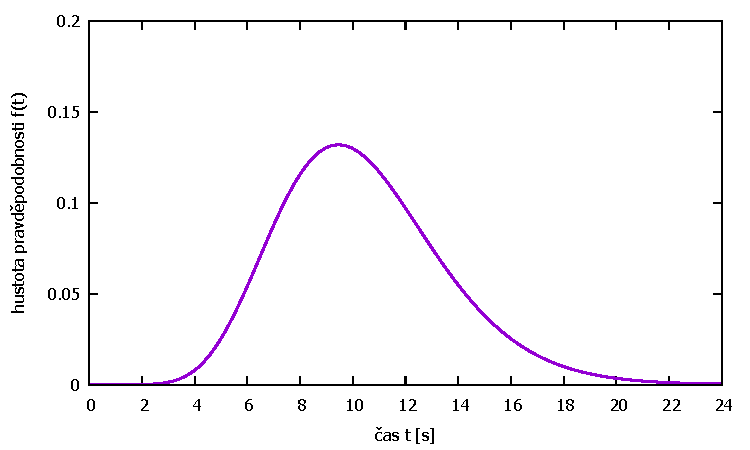
\includegraphics{doc/obrazky-figures/gamma_distribution.pdf}
    \caption{Pravděpodobnostní rozdělení gama s~parametry $\alpha = 10{,}95$ a~$\beta = 0{,}95$. Toto rozdělení bylo použito pro výběr doby trvání mezi sebráním bonusu a~vygenerováním dalšího bonusu.}
    \label{fig:probability-bonus-countdown}
\end{figure}

\subsection*{Vygenerování nových bonusů}

V~této fázi se nejdříve zkontroluje, zda odpočet pro vygenerování nového bonusu uplynul. Pokud ano, vygeneruje se nový bonus s~pomocí třídy \texttt{StageBonuses}. Tato třída je popsána v~kapitole~\ref{sec:jadro-hry}.

Vizuálním výstupem této fáze je přidání nového bonusu na herní plochu.


\section{Entity řízené počítačem}
\label{sec:entity-rizene-pocitacem}

Vytvořit entity řízené počítačem bylo jedním z~hlavních cílů této práce. Entity využívají metody popsané v~kapitole~\ref{ch:umela-inteligence} pro rozhodování svých dalších kroků. Bylo vytvořeno několik typů entit, které se liší svým cílem a~způsobem, jakým se snaží svého cíle dosáhnout. Uživatel má možnost tyto entity začlenit do hry během nastavení hry. Toto bylo popsáno v~kapitole~\ref{sec:uzivatelske-rozhrani}.

\subsection{Prostředí hry}

V~kapitole~\ref{sec:reseni-uloh} byly popsány různé vlastnosti, podle kterých lze kategorizovat prostředí úlohy pro umělou inteligenci. V~této sekci bude prostředí hry \emph{Bubble Brawl} rozděleno podle těchto vlastností do příslušných kategorií.

\subsubsection*{Pozorovatelnost}

Prostředí hry \emph{Bubble Brawl} má velmi blízko \emph{plné pozorovatelnosti}, avšak zařazení hry do této kategorie brání bonusy. U~bonusů hráči nemohou zjistit, jaké množství života jim bude při sebrání doplněno. Také časovač pro generování bonusů běží na pozadí a~hráči tak nemohou zjistit, za jak dlouhou dobu bude vygenerován další bonus. Proto prostředí této hry spadá spíše do kategorie \emph{částečně pozorovatelných}.

Hovořilo se však o~tom, že u~\emph{plně pozorovatelných} prostředí má každý hráč přehled o~všech \emph{relevantních} aspektech stavu hry. Hráče nemusí při plánování akcí zajímat, jaké množství života mu bonus doplní. Co se týče generování bonusů, hráč nemusí vědět o~tom, že nějaký časovač existuje a~generování chápat jako čistě náhodnou událost. V~takovém případě nemusí hráč nahlížet na generování bonusů jako na \emph{nepozorovatelný} aspekt, ale na čistě \emph{stochastický}. Pokud tyto 2 zmíněné aspekty přestanou být pro hráče relevantní, pak může na prostředí hry nahlížet jako na \emph{plně pozorovatelné}.

\subsubsection*{Množství agentů}

Je jasné, že prostředí hry \emph{Bubble Brawl} je \emph{multiagentní}. Otázkou však je, zda je možné toto prostředí jednoznačně zařadit do kategorie \emph{konkurenčních} prostředí. Pravidla hry totiž \emph{neznemožňují} vytváření \emph{neformálních aliancí} \cite[s.\,166]{AI_Russel_Norvig}, díky kterým jeden agent vykonáním jedné akce může zvýšit \emph{míru výkonnosti} jak sobě, tak dalším agentům ze stejné aliance (například, 3 slabší hráči mohou cíleně zaútočit na jednoho silnějšího hráče). Pro tyto případy je nejlepší o~prostředí hry hovořit pouze jako o~\emph{multiagentním} a~dále nespecializovat.

\subsubsection*{Determinizmus}

Prostředí hry \emph{Bubble Brawl} je \emph{stochastické}; opět kvůli bonusům. Ačkoliv velká část následujícího stavu hry závisí na aktuálním stavu, generování bonusu i~určení množství života získaného z~bonusu jsou stochastické jevy. Nicméně, žádný z~aktuálně implementovaných agentů nebere na tyto jevy zřetel právě kvůli tomu, jak velkou část následujícího stavu lze odvodit ze stavu aktuálního.

\subsubsection*{Návaznost akcí}

Prostředí hry \emph{Bubble Brawl} jednoznačně patří do kategorie \emph{sekvenčních} prostředí. Přestože důsledky akcí nejsou tak dlouhodobé, jako například ve hře \emph{Šachy}, jednotlivé akce stále určitým způsobem ovlivňují budoucí rozhodování. Navíc, pokud agent nebude brát jako akci pouze stisk klávesy, ale přímo pohyb z~jednoho místa do jiného vzdálenějšího, důsledky budou daleko větší.

\subsubsection*{Proměnlivost}

Ačkoliv se na první pohled může zdát, že prostředí hry \emph{Bubble Brawl} je \emph{dynamické}, není tomu tak. Hra se nemůže posunout dále, dokud se každý hrající agent nerozhodne, jakou akci vykoná. Na druhou stranu, agenti jsou zpravidla implementováni tak, aby dobou svého rozhodování nezpomalovali průběh hry.

\subsubsection*{Diskrétní a spojité prostředí}

Stavový prostor hry je teoreticky spojitý\,--\,omezený pouze přesností reálných čísel v~procesoru. Někteří agenti si však tento prostor navzorkují \cite{MIT_OpenCourseWare:Incremental_Path_Planning} za účelem optimalizace hledání cesty v~tomto prostoru, a~prohledávají tedy \emph{diskrétní} stavový prostor. Jakým způsobem vzorkování probíhá je popsáno v~kapitole~\ref{sec:entity-rizene-pocitacem:tridy}.

Podle ostatních aspektů by prostředí mělo být \emph{diskrétní}. Čas se mění skokově (přibližně $60\times$ za sekundu) a~množina akcí, které agent může v~jednom okamžiku vykonat, je konečná.

\subsubsection*{Znalost}

Z~pohledu téměř všech agentů se dá říci, že prostředí hry \emph{Bubble Brawl} je \emph{známé}. Pouze \uv{slepí} agenti (\emph{Blind predator} a~\emph{Blind prey}) někdy nedokážou přesně odhadnout stav, do kterého se vykonáním určité akce přesunou.

\subsection{Třídy}
\label{sec:entity-rizene-pocitacem:tridy}

V~programu je obsaženo několik tříd, které zajišťují fungování umělé inteligence ve hře. Největší skupinou tříd jsou ty, které řídí chování entit\,--\,\emph{agenti} (pojem \emph{agent} byl popsán v~kapitole~\ref{sec:reseni-uloh}). Existují však také další třídy, které tito \emph{agenti} využívají pro své fungování.

Velmi důležité pro \emph{agenty} je rozhraní \texttt{GameStateAgentProxy}\footnote{Na rozdíl od většiny ostatních rozhraní v~programu nemá předponu \uv{\texttt{I}}. Důvodem je jednoduše přehlédnutí během návrhu, které se nakonec dostalo i~do implementace.}. Jeho účelem je umožnit \textbf{přístup k~aktuálnímu stavu hry}. Mimoto také obsahuje několik pomocných metod, jako například výpočet nové pozice hráče po vykonání akce. Konkrétní implementaci tohoto rozhraní poskytuje samotné jádro hry (třída \texttt{Core}). Rozhraní poskytuje následující metody:
\begin{itemize}
    \item \texttt{getPlayers()}\,--\,Tato metoda vrací informace o~všech hráčích ve hře. Je to asociativní pole (\texttt{std::unordered\_map}), kde klíče jsou unikátní identifikátory hráčů. Informace, které jsou o~hráčích poskytovány, jsou: pozice, množství života, rychlost, síla a~velikost.
    \item \texttt{getObstacles()}\,--\,Poskytuje přístup k~překážkám na herní ploše. Návratovou hodnotou \emph{není} seznam překážek, ale objekt typu \texttt{StageObstacles}, který přímo zprostředkovává interakci mezi hráči a~překážkami (viz kapitola~\ref{sec:jadro-hry}).
    \item \texttt{getStageGridModel()}\,--\,Poskytuje přístup k~\emph{mřížovému modelu} herní plochy, viz dále.
    \item \texttt{getPlayerMovementVector()}\,--\,Vypočítá vektor hráčova pohybu na základě jeho aktuální pozice, rychlosti a~požadované akce.
    \item \texttt{calculateNewPlayerPos()}\,--\,Určí novou pozici hráče na základě jeho pozice, rychlosti, požadované akce a~překážek na herní ploše.
\end{itemize}

Spousta agentů využívá třídu \texttt{StageGridModel}, která představuje \textbf{diskrétní model herní plochy} \cite{MIT_OpenCourseWare:Incremental_Path_Planning}. Při vytváření instance této třídy je konstruktoru předána množina všech překážek na herní ploše a~velikost herní plochy. Podle těchto informací je herní plocha navzorkována. Vzniká mřížka čtvercových buněk s~délkou strany 17~jednotek délky (tato délka odpovídá maximální délce posunu hráče během jednoho herního cyklu). Z~této mřížky jsou následně odstraněny buňky, které se překrývají s~překážkami.

U~každé buňky je možné zjistit souřadnice jejího středu, vzdálenost středu od nejbližší překážky a~nejvýše 8~buněk, se kterými daná buňka sousedí. Různí agenti si vybírají akci podle toho, jak blízko je dostane ke středu vybrané buňky. Vzdálenost buňky od nejbližší překážky využívají agenti, aby zjistili, zda dokážou projít danou buňkou.

Nejdůležitější pro implementaci \textbf{agentů} je rozhraní \texttt{IAIPlayerAgent}. Toto rozhraní obsahuje 4~metody:
\begin{itemize}
    \item \texttt{plan()}\,--\,Znamení agentovi, že může začít plánovat další akci.
    \item \texttt{assignProxy()}\,--\,Poskytne agentovi přístup k~aktuálnímu stavu hry (instanci rozhraní \texttt{GameStateAgentProxy}). Agent nemá možnost plánovat akce, dokud nemá možnost zjišťovat stav hry, a~proto musí být tato metoda zavolána před prvním voláním \texttt{plan()}.
    \item \texttt{kill()}\,--\,Ukončení činnosti agenta. Pokud agent funguje na principu \emph{vláken}, jsou všechna \emph{vlákna} ukončena.
    \item \texttt{getPlayerInput()}\,--\,Vrací agentem naplánovanou akci.
\end{itemize}

Rozhraní \texttt{IAIPlayerAgent} implementuje abstraktní třída \texttt{AIPlayerAgentBase}, ze které jsou odvozeny všechny další třídy implementující chování agentů. Tato třída byla navržena tak, aby plánování každého agenta využívalo paralelní zpracování pomocí \emph{vláken}. Nepovedlo se však implementovat funkční řešení tohoto návrhu, a~tedy veškeré plánování běží sériově.


\subsection{Jednotlivé typy entit}

Program obsahuje několik typů entit řízených počítačem, které se liší svým chováním. Cílem většiny entit je samozřejmě zvítězit, nicméně tento cíl je příliš abstraktní a~je nutné si jej rozdělit na menší dílčí cíle. Různé entity mají různé cíle, což se projevuje na jejich chování. Některé entity mohou mít stejné cíle, ale liší se v~postupu, jak jich dosáhnout.

Entity lze dle dílčích cílů rozdělit na 3 základní typy: \emph{predátoři}, kteří se snaží pouze útočit, \emph{kořisti}, které se snaží pouze utíkat, a~\emph{beruška}, která zdánlivě nemá cíl žádný. Entit stejných typů bylo implementováno více. Cílem bylo nahradit dříve implementované entity vylepšenými verzemi. Přesto však starší verze entit zůstaly v~aplikaci, aby lidé, kteří si hru zkusili zahrát, mohli posoudit, zda se vylepšení dané entity opravdu povedlo, nebo zda původní verze dokázala hrát hru lépe.

\emph{Predátoři} a~\emph{kořisti} jsou entity založené na ohodnocování hráčů. V~každém herním cyklu ohodnotí všechny soupeře podle jejich síly a~vzdálenosti mezi sebou a~daným soupeřem a~na základě získaných ohodnocení činí rozhodnutí. Všechny varianty \emph{predátorů} mají stejný postup ohodnocování soupeřů, a~sice:

\begin{eqnarray}
    \label{eq:opponent-health-predator}
    f_h(p) & = & 10 \cdot \frac{1}{h(p)} \\
    \label{eq:opponent-distance-predator}
    f_d(p) & = & 30 \cdot \frac{1}{d^2(p)} \\
    \label{eq:opponent-eval-predator}
    f(p) & = & f_h(p) + f_d(p)
\end{eqnarray}
Rovnice~\eqref{eq:opponent-health-predator} ukazuje výpočet ohodnocení hráče~$p$ podle množství jeho života, v~níž funkce $h(p)$ představuje aktuální množství života hráče~$p$. Rovnice~\eqref{eq:opponent-distance-predator} ukazuje výpočet ohodnocení hráče $p$ podle vzdálenosti od hodnotící entity, kde funkce $d^2(p)$ představuje druhou mocninu této vzdálenosti. Nakonec, rovnice~\eqref{eq:opponent-eval-predator} ukazuje výpočet celkového ohodnocení hráče~$p$. Jak množství života, tak vzdálenost jsou nepřímo úměrné příslušnému ohodnocení. To znamená, že čím nižší je množství života a~vzdálenost daného soupeře, tím lepší je jeho ohodnocení. Obě ohodnocení jsou navíc násobena konstantou větší než~1 za účelem ovlivnění jejich významnost ve výsledku. Tyto konstanty byly vybrány zcela nahodile. Důvodem použití druhé mocniny vzdálenosti je především vyvarování se výpočetně náročné operaci odmocňování (inspirace v~\cite{CGAL_Exact_Computation_paradigm}).

Podobný postup ohodnocování soupeřů mají všechny \emph{kořisti}:
\begin{eqnarray}
    \label{eq:opponent-health-prey}
    f_h(p) & = & -10 \cdot h(p) \\
    \label{eq:opponent-distance-prey}
    f_d(p) & = & -30 \cdot \frac{1}{d^2(p)} \\
    \label{eq:opponent-eval-prey}
    f(p) & = & f_h(p) + f_d(p)
\end{eqnarray}
Význam jednotlivých proměnných a~funkcí zůstává stejný, jako v~rovnicích výše. Soupeřovo množství života je tentokrát přímo úměrné a~vzdálenost nepřímo úměrná příslušnému ohodnocení. Jelikož jsou tentokrát obě ohodnocení násobena zápornou konstantou, jejich význam je opačný: čím vyšší množství života má soupeř, tím nižší je jeho ohodnocení (tím je nebezpečnější), a~čím vyšší je vzdálenost od něj, tím vyšší je jeho ohodnocení (tím je méně nebezpečný).

Následuje seznam entit a~popis jejich fungování. Jejich jména zde odpovídají jménům, jak jsou zobrazena v~aplikaci. Pouze entity \emph{Wall-aware BFS predator}, \emph{IDS predator} a~\emph{BFS predator} jsou vynechány ze seznamu entit v~aplikaci, protože jejich výkonnost byla příliš nízká. Tyto entity lze opět zařadit do seznamu zakomentováním příslušného řádku\footnote{Jde o~řádek \texttt{add\_compile\_definitions(EXCLUDE\_SLOW\_AGENTS)}.} v~souboru \texttt{CMakeLists.txt} a~opětovným sestavením aplikace.

\subsubsection*{Ladybug}

\emph{Ladybug} (\emph{beruška}) je jednou z~prvních implementovaných entit. Jejím jediným cílem je pohybovat se přirozeně. Entita se snaží neměnit směr příliš rychle a~občas se zastavit, což může připomínat pohyb hmyzu (odtud název). Implementace chování této entity je následující:
\begin{enumerate}
    \item S~pravděpodobností~$15/16$ vykonej stejnou akci, jakou jsi vykonala naposledy. Jinak pokračuj.
    \item Pro každý ze 4 směrů (nahoru, dolů, doleva, doprava) nastav stav \uv{stisknuto} s~pravděpodobností~$1/2$, jinak na \uv{nestisknuto} a~výslednou akci vykonej.
\end{enumerate}
Na začátku platí stav \uv{nestisknuto} pro všechny 4 směry, tedy žádný pohyb.

\subsubsection*{Blind predator a Blind prey}

Entity \emph{Blind predator} a~\emph{Blind prey} patří mezi entity, které plánují pouze jeden krok dopředu. V~každém kroku se snaží vykonat akci, díky které dosáhnou stavu s~nejlepším ohodnocením. Ohodnocení stavu je dáno součtem ohodnocení všech soupeřů pro daný stav. Implementace chování obou entit je velmi podobná; liší se pouze ve způsobu ohodnocování soupeřů:
\begin{enumerate}
    \item Pro každou z~9~akcí (pohyb jedním z~8~směrů nebo žádný pohyb) spočítej ohodnocení následníka aktuálního stavu dosažitelného vykonáním dané akce.
    \item Vykonej akci, která vede do stavu s~nejlepším ohodnocením.
\end{enumerate}

Přívlastek \emph{blind} (\emph{slepý}) souvisí s~tím, že při rozhodování neberou v~potaz překážky na herní ploše (\uv{nevidí je}). Vykonání akce pro ně tedy znamená posunout se požadovaným směrem o~vzdálenost \emph{přesně} danou množstvím jejich života. Důsledkem toho je, že pokud tyto entity narazí na překážku, budou se domnívat, že tam žádná překážka není a~zůstanou stát na místě.

\subsubsection*{Wall-aware predator a Wall-aware prey}

Entity \emph{Wall-aware predator} a~\emph{Wall-aware prey} jsou opět entity, které dokážou plánovat pouze jeden krok dopředu. Implementace jejich chování je téměř stejná, jako implementace jejich \emph{blind} protějšků. Rozdílem však je, že tyto entity dokážou vnímat překážky na herní ploše, a~jsou tedy lépe informované o~tom, jaký důsledek bude mít která jejich akce.

Zlepšení chování je pozorovatelné především u \emph{kořisti} (\emph{Wall-aware prey}). Pokud je pronásledována soupeřem podél zdi a~dostane se do rohu, dokáže v~některých případech změnit směr a~pohybovat se podél zdi kolmé k~původní zdi. Přesto, ve spoustě případů entita v~rohu uvízne. Ani \emph{predátorovi} (\emph{Wall-aware predator}) toto zlepšení příliš nepomůže; pokud pronásleduje svou oběť a~v~cestě mu stojí jen velmi malá překážka, většinou nezvládne najít cestu okolo ní.

\subsubsection*{Wall-aware BFS predator}

Tato entita kombinuje metodu \emph{slepého prohledávání do šířky} (\emph{BFS}) a~implementaci generování akcí stejnou jako \emph{Wall-aware predator}. Jejím cílem při výběru dalšího kroku není najít nejoptimálnější stav, ale vybrat sousední stav, který leží na cestě vedoucí k~jednomu konkrétnímu soupeři. Entita si v~každém kroku vybírá nejlepší oběť a~počítá celou cestu vedoucí k~této oběti. Popis implementace chování entity je následující:
\begin{enumerate}
    \item Spočítej ohodnocení všech svých soupeřů pro aktuální stav a~vyber soupeře s~nejlepším ohodnocením jako svoji \emph{oběť}.
    \item Pokud se s~\emph{obětí} už dotýkáš, nevykonávej žádnou akci. Jinak pokračuj.
    \item Pomocí metody \emph{BFS s~kolekcí CLOSED} najdi cestu vedoucí z~tvojí aktuální pozice k~vybrané \emph{oběti}. Cílovou podmínkou budiž situace, kdy se při vykonání akce dotkneš svojí \emph{oběti}.
    \item Pokud nebyl nalezen cílový uzel, nevykonávej žádnou akci. Jinak pokračuj.
    \item Z~cílového uzlu najdi cestu vyhledávacím stromem zpět k~uzlu, který je bezprostředním následníkem kořene. Vykonej akci vedoucí z~kořenového uzlu do tohoto následníka.
\end{enumerate}

Entita má poměrně dobré znalosti o~důsledcích svých akcí. Na rozdíl od entit plánujících pouze jeden krok dopředu zná celou cestu až ke svojí oběti a~na rozdíl od entit využívající diskrétní model herní plochy dokáže projít i~úzkými průchody, které tyto entity mohou vyhodnotit jako neprůchozí. Velkou nevýhodou této entity je však dlouhá doba plánování. I~při velmi krátkých vzdálenostech od svého cíle trvá plánování entity nepřijatelně dlouhou dobu, jak je ukázáno v~kapitole~\ref{sec:vykonnostni-testovani}.

\subsubsection*{IDS predator}

Tato entita využívá diskrétní model herní plochy, na němž hledá cestu ke svojí \emph{oběti} pomocí metody \emph{postupného zanořování do hloubky} (\emph{IDS}). V~implementaci však není použito klasické \emph{IDS}; zatímco běžná implementace této metody opakovaně volá metodu \emph{slepého prohledávání do hloubky} (\emph{DFS}) s~omezenou hloubkou stromu, v~implementaci chování této entity je místo toho opakovaně volána metoda \emph{zpětného navracení} (\emph{Backtracking}). Záměrem bylo více optimalizovat paměťovou náročnost algoritmu. Popis implementace chování entity je následující:
\begin{enumerate}
    \item Spočítej ohodnocení všech svých soupeřů pro aktuální stav a~vyber soupeře s~nejlepším ohodnocením jako svoji \emph{oběť}.
    \item Pokud se \emph{oběť} nachází ve stejné buňce jako ty, nevykonávej žádnou akci. Jinak pokračuj.
    \item Pomocí modifikované metody \emph{IDS} najdi cestu vedoucí z~buňky, v~níž se nacházíš, do buňky, v~níž se nachází tvoje \emph{oběť}.
    \item Pokud nebyl nalezen cílový uzel, nevykonávej žádnou akci. Jinak pokračuj.
    \item Vykonej akci podle toho, v~jakém směru od kořenového uzlu se nachází jeho bezprostřední následník.
\end{enumerate}

V~každém uzlu může agent vykonat pouze 4~akce (svislý a~vodorovný pohyb) místo obvyklých 8. Původní myšlenka byla taková, že při diagonálních akcích nelze s~jistotou říci, zda průchod mezi diagonálně sousedícími buňkami je dostatečně široký. Tento problém se však týká i~svisle a~vodorovně sousedících buněk. Nakonec však toto omezení zůstalo z~důvodu snížení faktoru větvení vyhledávacího stromu, a~tedy urychlení plánování agentů.

Doba plánování entity je sice kratší, nicméně stále není dostatečně krátká, aby se dala považovat za přijatelnou. Testy však ukázaly, že prostorová náročnost při plánování je zanedbatelná oproti náročnosti časové (viz kapitola~\ref{sec:vykonnostni-testovani}). Proto se ostatní entity zaměřují na optimalizaci doby plánování na úkor využitého množství paměti.

\subsubsection*{BFS predator}

Implementace chování entity \emph{BFS predator} je ve většině ohledů stejná, jako implementace chování entity \emph{IDS predator}. Jediný rozdíl je použití metody \emph{slepého prohledávání do šířky s~kolekcí CLOSED} (\emph{BFS s~kolekcí CLOSED}) místo metody \emph{IDS}.

Díky velkému snížení počtu generování uzlů se mnohonásobně zkrátila doba plánování, jak je ukázáno v~kapitole~\ref{sec:vykonnostni-testovani}. Tato optimalizace téměř stačí na to, aby byla entita považována za začlenitelnou do hry. Problémem však stále zůstává, že entita není \emph{stabilní}. Doba plánování entity není omezena, a~proto na větších herních plochách může stále zpomalovat běh programu.

\subsubsection*{A* predator}

Entita \emph{A* predator} se stále implementačně podobá entitám \emph{IDS predator} a~\emph{BFS predator}. Základní algoritmus je téměř stejný, pouze s~obměnou metody \emph{IDS}/\emph{BFS} za metodu \emph{A*}. Nastalo však několik dalších změn.

Tato entita hledá cestu ke svojí oběti, ale přestane hledat, jakmile vygeneruje 5\,000.~uzel. Tato změna zaručuje, že plánování agenta bude \emph{stabilní}, tady ani na příliš velkých herních plochách by neměla zpomalovat běh programu. Číslo 5\,000 bylo vybráno na základě testování tak, aby při hře 8~hráčů tohoto typu běžela aplikace dostatečně rychle i~na méně výkonných počítačích. Po vygenerování tohoto množství uzlů však není prohledávání rovnou ukončeno jako neúspěšné. Jak se má postupovat dále je určeno verzí entity.

Entita \emph{A* predator} byla několikrát vylepšena, ale předchozí implementace v~kódu zůstaly. Jejich aktivace je možná nastavením hodnoty makra \texttt{ASTAR\_PREDATOR\_VERSION} v~souboru \texttt{AstarPredatorAIPlayerAgent.hpp}. Verze 1~entity po dosažení maximálního počtu vygenerovaných uzlů zvolí uzel na vrcholu kolekce \emph{OPEN} jako cílový uzel. To samé činí i~verze~2 této entity. Vylepšení v~této verzi naopak spočívá ve výběru akce po dokončení hledání cesty. Entita \uv{vyzkouší} vykonat všech 8~možných pohybů a~vybere si ten, který ji dostane nejblíže k~bezprostřednímu následníku kořenového uzlu. Poslední, 3. verze entity opět mění způsob výběru cílového uzlu po vygenerování maximálního počtu uzlů. Vybrán je ten, jehož ohodnocení heuristikou $h(s_k)$ je ze všech uzlů v~kolekci \emph{CLOSED} nejnižší (jinými slovy, jehož vzdálenost od cílového uzlu je nejnižší).

Entita je velmi schopná v~plnění svého cíle, tedy v~pronásledování svojí oběti. I~přes omezení počtu vygenerovaných uzlů má velkou šanci zvolit správnou cestu v~případě, že po dosažení tohoto limitu nedorazí do cílového uzlu. Také doba plánování této entity je velmi uspokojivá. Ovšem nevýhodou je velmi malá šance na přežití. Jelikož se entita snaží pouze útočit a~nevyhledává bonusy, je jednoduché ji velice brzy vyřadit ze hry.

\subsubsection*{Minimax prey}

Entita \emph{Minimax prey} se snaží hledat optimální stav pomocí metody \emph{Minimax}. Vybírá si soupeře, který ji nejvíce ohrožuje, jako útočníka. Následně se snaží předpovědět jeho chování, a~podle toho pak hledat optimální stav. Entita opět používá diskrétní model herní plochy pro plánování. Popis implementace chování entity je následující:
\begin{enumerate}
    \item Spočítej ohodnocení všech svých soupeřů pro aktuální stav a~vyber soupeře s~nejhorším ohodnocením jako svého \emph{útočníka}.
    \item Pomocí metody \emph{Minimax} najdi optimální stav. Hráč \emph{Max} jsi ty, hráč \emph{Min} je tvůj \emph{útočník}.
    \item Urči bezprostředního následníka kořenového uzlu, který leží na cestě k~nalezenému optimálnímu stavu. Vykonej pohyb, který tě k~tomuto následníku dostane nejblíže.
\end{enumerate}

Opět bylo vyvinuto několik verzí této entity\,--\,konkrétně 2. Nastavit jinou lze změnou hodnoty makra \texttt{MINIMAX\_PREY\_VERSION} v~souboru \texttt{MinimaxPreyAIPlayerAgent.hpp}. Tyto verze se liší pouze v~použité metodě hledání cesty. První verze používá obyčejnou metodu \emph{Minimax}, verze~2 pak metodu \emph{Alfa-beta řezů}.

Ačkoliv je metoda \emph{Minimax} určena především pro hry, kde se hráči na tahu střídají, povedlo se ji implementovat i~pro tuto hru. Aby však plánování netrvalo příliš dlouho musela být maximální hloubka vyhledávacího stromu stanovena na velmi malé číslo. Verze~1, která používá obyčejnou metodu \emph{Minimax}, má nastavenou maximální hloubku 6, druhá verze, která využívá \emph{Alfa-beta řezy}, má nastavenou maximální hloubku 8. Jak je ukázáno v~kapitole~\ref{sec:vykonnostni-testovani}, větší hodnoty hloubky by mohly zpomalovat běh programu. Kvůli nízké hloubce vyhledávacího stromu nemá tato entita o~mnoho lepší schopnosti, než \uv{slepá} entita \emph{Wall-aware prey}.

\subsection{Nevyužité metody řešení úloh}

V~kapitole~\ref{ch:umela-inteligence} bylo představeno několik metod řešení úloh a~hraní her. Spousta z~nich byla použita pro implementaci chování entit řízených počítačem, ale některé se do implementace nedostaly. Tato sekce se věnuje důvodům, proč nebyly tyto metody v~implementaci použity.

Z~neinformovaných metod prohledávání stavového prostoru byly v~práci použity pouze 2: \emph{slepé prohledávání do šířky} (\emph{BFS}) a~\emph{postupné zanořování do hloubky} (\emph{IDS}). Ostatní jsou v~práci použity nepřímo, například \emph{zpětné navracení} (\emph{Backtracking}) a~\emph{omezené prohledávání do hloubky} (\emph{DLS}) jako součást metody \emph{IDS}, nebo \emph{slepé prohledávání do hloubky} (\emph{DFS}) jako součást metody \emph{Minimax}. Jediná neinformovaná metoda, kterou se nepodařilo využít ani nepřímo, je metoda \emph{stejných cen} (\emph{UCS}). Žádná z~entit nepoužívá při hledání cesty ohodnocení přechodů mezi stavy, a~tudíž by se tato metoda neuplatnila.

Z~informovaných metod byla využita pouze jedna, a~to metoda \emph{A*}. Ostatní informované metody pouze zvyšují výkonnost metody \emph{A*}. Jelikož entita využívající tuto metodu (entita \emph{A* predator}) plánuje velmi rychle, nebylo nutné ji dále vylepšovat. Mimoto u~některých metod se později ukázalo, že nejsou příliš vhodné pro tento typ úlohy. Aby se projevila účinnost metody \emph{Lifelong Planning A*}, musely by entity brát v~úvahu přechody mezi stavy. To stejné platí i~pro metodu \emph{D* Lite}. Navíc tato metoda vyžaduje, aby v~každém jejím volání (tedy v~každém herním cyklu) zůstal cílový uzel stejný. Jelikož cílem jsou většinou ostatní hráči, kteří se po herní ploše pohybují, tato metoda by v~tomto případě použitelná vůbec nebyla. Metoda \emph{Anytime Repairing A*} vyžaduje, aby napříč jejími voláními (napříč herními cykly) zůstal stav úlohy stejný, což v~multiagentních prostředích zaručit nelze.

Metody hraní her byly v~aplikaci použity 2: \emph{Minimax} a~\emph{Alfa-beta řezy}. Metody \emph{Max\textsuperscript{n}} a~\emph{Shallow pruning} nebylo možné využít především z~výkonnostních důvodů. Samy \emph{Minimax} i~\emph{Alfa-beta řezy} byly pro tuto hru příliš výkonnostně náročné. Metody \emph{Max\textsuperscript{n}} a~\emph{Shallow pruning} generují oproti nim mnohem větší počet uzlů, a~mají tedy větší časové nároky. Z~toho bylo možné usoudit, že tyto metody v~implementaci chování entit neobstojí.


\chapter{Testování}
\label{ch:testovani}

Tato kapitola se zabývá zhodnocením funkčnosti výsledného programu. Pro zhodnocení byly použity dva přístupy. První část této kapitoly se věnuje testování výkonnosti programu. Zaměřuje se především na výkonnostní testování jádra hry a~entit řízených počítačem. Druhá část této kapitoly se pak věnuje zpětné vazbě od uživatelů, kteří si vyzkoušeli používání aplikace.

\section{Výkonnostní testování}
\label{sec:vykonnostni-testovani}

V~této sekci jsou ukázány výsledky měření výkonnosti různých částí aplikace. Cílem měření bylo především zjistit, jak implementovat entity řízené počítačem, aby nezpomalovaly chod aplikace. Měřen byl čas strávený při vykonávání různých funkcí v~programu. Pokud není řečeno jinak, pak testy byly provedeny v~prostředí s~těmito vlastnostmi:
\begin{itemize}
    \item operační systém: Windows 11 Pro, verze 23H2,
    \item procesor: AMD Ryzen 7 5700U with Radeon Graphics, 1.80 GHz,
    \item RAM: 16 GB.
\end{itemize}
Na pozadí běžely další procesy, jako například antivirus, internetový prohlížeč aj., aby zátěž byla přibližně taková, jaká by mohla být při běžném používání aplikace. Pro měření byla použita třída \texttt{Benchmark} ze souboru \texttt{utility/benchmark/Benchmark.hpp}. Ve výsledné aplikaci je tato třída vyřazena ze sestavování; pro její začlenění do aplikace lze nastavit v~souboru \texttt{CMakeLists.txt} proměnnou \texttt{INCLUDE\_BENCHMARK} na hodnotu \texttt{TRUE} (příkaz \texttt{set(INCLUDE\_BENCHMARK TRUE)}). Stojí za připomenutí, že doba mezi herními cykly je 17\,ms. V~ideálním případě by tedy vše, co souvisí s~herním cyklem, mělo být vykonáno během této doby.

\subsection*{Hra bez umělých hráčů}

Tabulka~\ref{tab:benchmark-basics} ukazuje průměrnou dobu trvání vykonání všech kroků herního cyklu (řádek \uv{Změna stavu hry}) a~vizuální výstup těchto změn (řádek \uv{Výstup na obrazovku}). Ve hře bylo vždy 8 hráčů a~každá průměrná hodnota byla vypočítána z~přibližně 300 záznamů měření (přibližně 5,1\,s běhu programu). Pro testování byly použity tyto 2 herní plochy: \emph{Too many players} a~\emph{Shattered glass}. Důvodem výběru těchto 2 herních ploch je počet překážek\,--\,zatímco \emph{Too many players} nemá překážku žádnou, \emph{Shattered glass} jich má 51. Díky tomuto lze dobře porovnat vliv množství překážek na výkon aplikace. Tabulka se na tyto herní plochy neodkazuje jejich jménem, ale přímo počtem překážek.

\begin{table}[ht]
    \centering
    \begin{tabular}{|l|c|c|} \hline
        \textbf{Počet překážek}      & \textbf{0} & \textbf{51} \\ \hline\hline
        \textbf{Změna stavu hry}     & 0,031      & 0,057       \\ \hline
        \textbf{Výstup na obrazovku} & 3,581      & 5,327       \\ \hline
    \end{tabular}
    \caption{Průměrná doba trvání základních operací souvisejících s~herním cyklem (v~milisekundách).}
    \label{tab:benchmark-basics}
\end{table}

Z~testu lze vypozorovat, že herní cyklus samotný není příliš výkonnostně náročný, a~to ani při rostoucím množství překážek. Naopak, zobrazení stavu hry na obrazovce zabere poměrně výraznou část doby mezi herními cykly\,--\,více než 20\,\%. S~přidáním většího množství překážek také poměrně výrazně vzrostla doba zpracování\,--\,přibližně o~10\,\% doby mezi herními cykly.

Pokud entita řízená počítačem má být použita v~aplikaci, pak doba, kterou stráví plánováním, by měla být menší než $11{,}673\text{\,ms} = 17\text{\,ms} - 5{,}327\text{\,ms}$. Tuto dobu může entita strávit plánováním, pokud bude ve hře pouze 1. Maximální počet hráčů ve hře je však 8, a~proto, pokud by mělo být zapojeno 8~entit daného typu, měla by být doba plánování maximálně $1{,}46\text{\,ms} = 11{,}673\text{\,ms} : 8$. Tyto časy jsou shrnuty v~tabulce~\ref{tab:times-summary}.

\begin{table}[ht]
    \centering
    \begin{tabular}{|p{0.4\textwidth}|c|} \hline
         & \textbf{Čas [ms]} \\ \hline
        \textbf{Doba mezi herními cykly}                    & 17    \\ \hline
        \textbf{Přibližná doba trvání výstupu na obrazovku} & 5,327 \\ \hline
        \textbf{Maximální doba plánování 1~agenta (při hře 1~agenta)} & 11,673 \\ \hline
        \textbf{Maximální doba plánování 1~agenta (při hře 8~agentů)} & 1,46   \\ \hline
    \end{tabular}
    \caption{Shrnutí časů potřebných pro vykonání různých akcí.}
    \label{tab:times-summary}
\end{table}

\subsection*{Jednoduší agenti}

Tabulka~\ref{tab:benchmark-simple-bots} ukazuje průměrnou dobu plánování agentů typu \emph{Ladybug}, \emph{Blind predator} a~\emph{Blind prey}. Tito agenti nevyužívají při plánování ani překážky na herní ploše, ani diskrétní model herní plochy. Je tedy zřejmé, že doba plánování nebude ovlivněna počtem překážek, nicméně kvůli konzistentnosti jsou data v~tabulce opět rozdělena do 2 sloupců podle tohoto kritéria. Asi není žádným překvapením, že doba plánování těchto agentů je velmi krátká. \emph{Ladybug} používá pouze generátor náhodných čísel a~bitové operace. \emph{Blind predator} a~\emph{Blind prey} sice používají náročnější aritmetické operace a~doba jejich plánování je tím pádem zhruba 4\texttimes{} delší, ale i~přesto lze říct, že tato doba je naprosto zanedbatelná.

Pro testování byly použity herní plochy \emph{Too many players} a~\emph{Shattered glass} ze stejného důvodu, jako v~případě předcházejícího testu.

\begin{table}[ht]
    \centering
    \begin{tabular}{|l|c|c|} \hline
        \textbf{Počet překážek} & \textbf{0}  & \textbf{51} \\ \hline\hline
        \textbf{Ladybug}        & 0,000\,29   & 0,000\,29   \\ \hline
        \textbf{Blind predator} & 0,000\,98   & 0,001\,3    \\ \hline
        \textbf{Blind prey}     & 0,001       & 0,001       \\ \hline
    \end{tabular}
    \caption{Průměrná doba plánování jednoduchých agentů (v~milisekundách).}
    \label{tab:benchmark-simple-bots}
\end{table}

\subsection*{Wall-aware agenti}

Tabulka~\ref{tab:benchmark-wall-aware-bots} ukazuje průměrnou dobu plánování agentů typu \emph{Wall-aware predator} a~\emph{Wall-aware prey}. Tito agenti při plánování berou v~potaz překážky na herní ploše, ale plánují pouze jeden krok dopředu. Začlenění překážek do procesu rozhodování způsobuje, že činnost agenta trvá 2--3\texttimes{} delší dobu na herní ploše bez překážek a~více než 20\texttimes{} delší dobu s~51 překážkami. I~přesto zabere plánování těchto agentů přibližně 0,1\,\% z~celkové doby mezi herními cykly, tedy velmi zanedbatelné množství času. Z~tohoto důvodu fungují na podobném principu některé části implementace chování i~jiných typů agentů.

Pro testování byly použity tyto herní plochy \emph{Too many players} a~\emph{Shattered glass} ze stejného důvodu, jako v~případě předcházejících dvou testů.

\begin{table}[ht]
    \centering
    \begin{tabular}{|l|c|c|} \hline
        \textbf{Počet překážek}      & \textbf{0}  & \textbf{51} \\ \hline\hline
        \textbf{Wall-aware predator} & 0,002\,55   & 0,024\,23   \\ \hline
        \textbf{Wall-aware prey}     & 0,003\,69   & 0,027\,4    \\ \hline
    \end{tabular}
    \caption{Průměrná doba plánování \uv{wall-aware} agentů (v~milisekundách).}
    \label{tab:benchmark-wall-aware-bots}
\end{table}

\subsection*{Wall-aware BFS predator}

Tabulka~\ref{tab:benchmark-wall-aware-bfs-predator} obsahuje část výsledků měření výkonnosti agenta \emph{Wall-aware BFS predator}. Chování tohoto agenta je mírně odlišné od dosud testovaných agentů\,--\,zatímco předchozí agenti plánovali pouze jeden krok dopředu, \emph{Wall-aware BFS predator} plánuje celou cestu až ke své oběti. Proto nemělo cenu měřit průměrnou dobu plánování, jelikož každý proces plánování může trvat různě dlouhou dobu. Tabulka obsahuje 3 sloupce: hodnoty v~prvním sloupci představují vzdálenost mezi \emph{kružnicemi} hráčů, v~druhém sloupci počet vygenerovaných uzlů metodou \emph{BFS} a~ve třetím čas v~milisekundách strávený plánováním. Testování probíhalo pouze na herní ploše \emph{Too many players}; na ploše \emph{Shattered glass} nedokázal agent učinit rozhodnutí ani po 10~minutách plánování, a~testování tím pádem nedávalo příliš smysl (celkově, agent, který nedokáže učinit rozhodnutí ani do oněch 17\,ms času mezi herními cykly, je prakticky nepoužitelný).

\begin{table}[ht]
    \centering
    \begin{tabular}{|c|c|c|} \hline
        \textbf{Vzdálenost} & \textbf{Počet uzlů} & \textbf{Čas [ms]} \\ \hline
        84,39               & 9\,625\,778         & 11\,550,2    \\ \hline
        47,69               & 1\,225\,619         & 934,489      \\ \hline
        22,33               & 24\,110             & 11,396       \\ \hline
        11,09               & 1\,078              & 0.593        \\ \hline
    \end{tabular}
    \caption{Doba a~počet uzlů vygenerovaných během plánování agenta \emph{Wall-aware BFS predator} v~závislosti na vzdálenosti mezi jeho \emph{kružnicí} a~\emph{kružnicí} jeho oběti.}
    \label{tab:benchmark-wall-aware-bfs-predator}
\end{table}

Záznamy měření v~tabulce byly vybrány systematicky podle délky trvání. První záznam je nejdelší zaznamenaná doba plánování agenta během hry. Druhý záznam je první plánování, jehož doba je kratší než 1~sekunda. Třetí a~čtvrtý záznam jsou první plánování, které splňují maximální doby plánování 1~agenta podle tabulky~\ref{tab:times-summary}.

Už podle prvního záznamu lze usoudit, že tento agent není prakticky použitelný pro běžné hraní. Hráči od sebe mohou být na herní ploše vzdálení až 1000 jednotek vzdálenosti a~tento agent již při pouhých 84 jednotkách plánuje celých 11,5~sekundy.

Za povšimnutí stojí také rozdíl vzdálenosti a~počtu uzlů mezi prvním a~druhým záznamem. Zatímco vzdálenost je přibližně 2\texttimes{} nižší, počet uzlů klesl téměř o 9násobek. Zde se projevuje časová složitost metody \emph{BFS}\,--\,se zvyšující se hloubkou vyhledávacího stromu, v~níž se nachází cílový uzel, roste počet generovaných uzlů exponenciálně.

Tento test ukázal, že není výhodné provádět plánování opakovaným zkoušením vstupů z~klávesnice. Proto další agenti začali používat diskrétní model herní plochy, který pracuje efektivněji.

\subsection*{IDS predator}

Tabulka~\ref{tab:benchmark-ids-predator} obsahuje část výsledků měření výkonnosti agenta \emph{IDS predator}. Tento agent využívá při plánování diskrétní model herní plochy a~plánuje celou cestu až ke své oběti. Sloupce tabulky ukazují vzdálenost mezi pozicemi agenta a~jeho oběti, počet uzlů vygenerovaných metodou \emph{IDS} a~čas strávený plánováním. Záznamy měření byly vybírány stejným způsobem, jako v~případě agenta \emph{Wall-aware BFS predator}. Zde je však tabulka rozdělena na 2~části. V~první části byla použita herní plocha  \emph{Too many players}, v~druhé pak plocha \emph{Shattered glass}.

\begin{table}[ht]
    \centering
    \begin{tabular}{|c|c|c|} \hline
        \textbf{Vzdálenost} & \textbf{Počet uzlů} & \textbf{Čas [ms]} \\ \hline\hline
        \multicolumn{3}{|c|}{\textbf{Počet překážek: 0}}              \\ \hline
        184,39              & 38\,862\,057        & 3\,873,61         \\ \hline
        165,86              & 5\,346\,717         & 537,386           \\ \hline
        128,69              & 99\,989             & 10,359            \\ \hline
        117,83              & 5\,714              & 0,921             \\ \hline\hline
        \multicolumn{3}{|c|}{\textbf{Počet překážek: 51}}             \\ \hline
        266,83              & 108\,316\,298       & 10\,787           \\ \hline
        220,17              & 6\,647\,559         & 655,84            \\ \hline
        153,75              & 91\,528             & 9,446             \\ \hline
        116                 & 12\,352             & 1,197             \\ \hline
    \end{tabular}
    \caption{Doba a~počet uzlů vygenerovaných během plánování agenta \emph{IDS predator} v~závislosti na vzdálenosti od jeho oběti.}
    \label{tab:benchmark-ids-predator}
\end{table}

Je patrné, že tento agent plánuje mnohem rychleji, než \emph{Wall-aware BFS predator}. Přestože počet generovaných uzlů roste rychleji se zvyšující se vzdáleností od oběti, čas využitý při jejich generování a~prozkoumávání je mnohem nižší. Stále je však doba plánování příliš dlouhá i~pro malé vzdálenosti.

Dále je také vidět, že díky použití diskrétního modelu není doba výpočtu ovlivněna počtem překážek na herní ploše. Vzdálenosti všech buněk od překážek byly vypočítány před začátkem hry, a~agent nyní pouze porovnává svůj poloměr s~konkrétními hodnotami.

Test ukázal, že použití diskrétního modelu při plánování je velmi výhodné z~hlediska rychlosti plánování. Zároveň ukázal, že při použití tohoto modelu jsou požadavky na paměť daleko menší oproti požadavkům na dobu plánování\,--\,za přijatelnou dobu je možné vygenerovat přibližně 16\,000 uzlů. Proto nedává smysl používat metody, které jsou navrženy tak, aby šetřily paměť (a~mezi něž patří i~metoda \emph{IDS}).

\subsection*{BFS predator}

Agent \emph{BFS predator} využívá při plánování diskrétní model herní plochy a~plánuje celou cestu až ke své oběti pomocí metody \emph{BFS s~kolekcí CLOSED}. Tabulka~\ref{tab:benchmark-bfs-predator-compare-ids} ukazuje část výsledků měření jeho výkonnosti, jejíž sloupce obsahují vzdálenost od vybrané oběti, počet uzlů vygenerovaných metodou \emph{BFS} a~čas strávený plánováním v~tomto pořadí. Test probíhal pouze na herní ploše \emph{Too many players}. Tabulka~\ref{tab:benchmark-bfs-predator-limits} také ukazuje část výsledků měření výkonnosti tohoto agenta, ale první sloupec tentokrát obsahuje rozměry herní plochy, na níž probíhalo testování. Tento test probíhal na herní ploše \emph{Enormous stage} s~upravenými rozměry.

\begin{table}[ht]
    \centering
    \begin{tabular}{|c|c|c|} \hline
        \textbf{Vzdálenost} & \textbf{Počet uzlů} & \textbf{Čas [ms]} \\ \hline
        184,39              & 1\,688              & 0,473             \\ \hline
        165,86              & 1\,320              & 0,293             \\ \hline
        128,69              & 680                 & 0,158             \\ \hline
        117,83              & 316                 & 0,086             \\ \hline
    \end{tabular}
    \caption{Doba a~počet uzlů vygenerovaných během plánování agenta \emph{BFS predator} v~závislosti na vzdálenosti od jeho oběti.}
    \label{tab:benchmark-bfs-predator-compare-ids}
\end{table}

\begin{table}[ht]
    \centering
    \begin{tabular}{|c|c|c|} \hline
        \textbf{Rozměry HP}       & \textbf{Počet uzlů} & \textbf{Čas [ms]} \\ \hline
        11\,800\texttimes{}6\,000 & 954\,945            & 988,216           \\ \hline
        2\,800\texttimes{}1\,700  & 59\,785             & 11,391            \\ \hline
        1\,000\texttimes{}750     & 8\,057              & 1,333             \\ \hline
    \end{tabular}
    \caption{Doba a~počet uzlů vygenerovaných během plánování agenta \emph{BFS predator} v~závislosti na velikosti herní plochy (HP).}
    \label{tab:benchmark-bfs-predator-limits}
\end{table}

Záznamy pro první tabulku byly vybírány tak, aby vzdálenosti v~levém sloupci odpovídaly vzdálenostem v~první části tabulky~\ref{tab:benchmark-ids-predator}. Je zde totiž vidět markantní snížení počtu generovaných uzlů a~doby plánování. Metoda \emph{BFS} úplně předchází opakovanému generování uzlů díky použití kolekce (množiny) \emph{CLOSED}. Naopak metoda \emph{IDS} generuje většinu uzlů víckrát. K~tomu dochází nejen z~důvodu opakovaného volání metody \emph{DLS} a~absence kolekce \emph{CLOSED}, ale~navíc také kvůli způsobu implementace metody \emph{IDS} v~chování agenta \emph{IDS predator}. Typická implementace metody \emph{IDS} opakovaně volá metodu \emph{DLS} vycházející z~metody \emph{DFS}. Avšak kvůli snaze snížit paměťovou náročnost byla v~implementaci tohoto agenta využita varianta metody \emph{DLS} vycházející z~metody \emph{Backtracking}. Důsledkem této volby je to, že kolekce \emph{OPEN} obsahuje velmi malé množství uzlů, a~spousta uzlů je kvůli tomu generována i~přesto, že dříve již generovány byly.

Záznamy pro druhou tabulku byly vybírány\,--\,podobně jako u~předchozích agentů\,--\,tak, aby čas představoval vybrané limitní hodnoty. Konkrétně, první řádek představuje plánování s~dobou trvání mírně pod 1~sekundou, druhý řádek plánování s~dobou přípustnou pro maximálně jednoho agenta typu \emph{BFS predator} a~třetí řádek plánování dostatečně krátké pro hru 8~agentů tohoto typu (limity pro druhý a~třetí řádek jsou stanoveny v~tabulce~\ref{tab:times-summary}). Při testování byly hledány rozměry herní plochy takové, aby průměrná doba plánování agenta splňovala výše uvedené požadavky. Během testu bylo zaručeno, že agent nebude schopen najít svého soupeře, a~tím pádem prohledá celý stavový prostor. Z~měření je patrné, že doba zpracování připadající na 1~uzel je delší u~tohoto agenta než u~agenta \emph{IDS predator}. Agent \emph{BFS predator} totiž oproti agentovi \emph{IDS predator} používá navíc kolekci \emph{CLOSED} a~také kolekce \emph{OPEN} během plánování dosáhne většího počtu uzlů. To způsobí několik realokací těchto kolekcí. Avšak v~porovnání s~ušetřeným množstvím generování uzlů touto metodou je toto mírné prodloužení výpočtu na uzel zanedbatelné.

Testování ukázalo, že kolekce \emph{CLOSED} velmi výrazně pomáhá zkrátit dobu plánování. Problémem však stále zůstává, že na průměrně velkých herních plochách může být doba plánování v~některých případech nepřijatelně dlouhá.

\subsection*{A* predator}

Agent \emph{A* predator} využívá při plánování diskrétní model herní plochy a~plánuje pouze část cesty ke své oběti. Tabulka~\ref{tab:benchmark-astar-predator-compare-ids} ukazuje část výsledků měření jeho výkonnosti, jejíž sloupce obsahují vzdálenost od vybrané oběti, počet uzlů vygenerovaných metodou \emph{A*} a~čas strávený plánováním v~tomto pořadí. Tento test probíhal pouze na herní ploše \emph{Too many players} a~používal verzi~3 agenta \emph{A* predator}. Tabulka~\ref{tab:benchmark-astar-predator-versions} ukazuje průměrně doby plánování různých verzí agenta \emph{A* predator}. Sloupce představují měření na herních plochách \emph{Enormous stage (locked)} (počet překážek:~1) a~\emph{Shattered glass (locked)} (počet překážek:~51).

\begin{table}[ht]
    \centering
    \begin{tabular}{|c|c|c|} \hline
        \textbf{Vzdálenost} & \textbf{Počet uzlů} & \textbf{Čas [ms]} \\ \hline
        184,39              & 65                  & 0,048             \\ \hline
        165,86              & 57                  & 0,038             \\ \hline
        128,69              & 41                  & 0,034             \\ \hline
        117,83              & 29                  & 0,03              \\ \hline
    \end{tabular}
    \caption{Doba a~počet uzlů vygenerovaných během plánování agenta \emph{A* predator} v~závislosti na vzdálenosti od jeho oběti.}
    \label{tab:benchmark-astar-predator-compare-ids}
\end{table}

\begin{table}[ht]
    \centering
    \begin{tabular}{|c|c|c|} \hline
        \textbf{Počet překážek} & \textbf{1}  & \textbf{51} \\ \hline\hline
        \textbf{verze 1}        & 0,951       & 0.973       \\ \hline
        \textbf{verze 2}        & 0,951       & 0.921       \\ \hline
        \textbf{verze 3}        & 0,942       & 0.956       \\ \hline
    \end{tabular}
    \caption{Průměrná doba plánování různých verzí agenta \emph{A* predator} (v~milisekundách).}
    \label{tab:benchmark-astar-predator-versions}
\end{table}

První tabulka opět slouží pro porovnání s~dříve testovanými agenty. Záznamy zde byly vybírány tak, aby vzdálenosti v~levém sloupci odpovídaly vzdálenostem v~tabulce~\ref{tab:benchmark-bfs-predator-compare-ids} a~v~první části tabulky~\ref{tab:benchmark-ids-predator}. Je zde opět vidět velké zlepšení oproti agentovi \emph{BFS predator}. Toto zlepšení sice není natolik markantní jako mezi agentem \emph{IDS predator} a~\emph{BFS predator}, nicméně, je zde velmi dobře vidět účinnost informované metody oproti neinformovaným.

Druhá tabulka slouží pro porovnání různých verzí agenta \emph{A* predator}. Jelikož se napříč verzemi pouze zlepšovaly schopnosti agenta, a~nikoliv rychlost plánování, je vhodné ověřit, zda se nezhoršila výkonnost aplikace při přechodu na jinou verzi. Testování záměrně probíhalo na velkých herních plochách, v~nichž agent nemá možnost dosáhnout svojí oběti. Tím pádem využil všech 6\,000 stavů, které má při plánování k~dispozici. Měření potvrzuje očekávání, a~sice že napříč verzemi agenta není zřetelné žádné zhoršení výkonnosti.

\subsection*{Minimax prey}

Agent \emph{Minimax prey} využívá při plánování diskrétní model herní plochy a~pomocí metody \emph{Minimax} se snaží najít stav, ve kterém se co nejvíce vzdálí od jednoho vybraného útočníka. Tabulka~\ref{tab:benchmark-minimax-prey-versions} ukazuje průměrně doby plánování různých verzí tohoto agenta s~různě nastavenou maximální hloubkou vyhledávacího stromu. Sloupce představují měření na herních plochách \emph{Enormous stage (together)} (počet překážek:~0) a~\emph{Shattered glass} (počet překážek:~51).

\begin{table}[ht]
    \centering
    \begin{tabular}{|c|c|c|c|} \hline
        \multicolumn{2}{|c|}{\textbf{Počet překážek}} & \textbf{0} & \textbf{51} \\ \hline\hline
        \multirow{2}{*}{\textbf{verze 1}} & \textbf{hloubka 6} & 0,425 & 0,275 \\ \cline{2-4}
                                          & \textbf{hloubka 7} & 1,87  & 1,065 \\ \hline
        \multirow{2}{*}{\textbf{verze 2}} & \textbf{hloubka 8} & 0,707 & 0,261 \\ \cline{2-4}
                                          & \textbf{hloubka 9} & 1,81  & 0,632 \\ \hline
    \end{tabular}
    \caption{Průměrná doba plánování (v~milisekundách) různých verzí agenta \emph{Minimax prey} s~různými nastaveními maximální hloubky metody \emph{Minimax}.}
    \label{tab:benchmark-minimax-prey-versions}
\end{table}

Hloubky vyhledávacího stromu byly vybrány tak, aby bylo zřejmé, že hodnota použitá v~implementaci chování agenta je skutečně nejvyšší možná. První hloubka u~každé verze tedy představuje hloubku použitou v~implementaci, druhá pak hloubku o~1~vyšší. Aby hru mohlo hrát 8~agentů typu \emph{Minimax prey}, musí být doba plánování nižší než 1,46\,ms (viz tabulka~\ref{tab:times-summary}). Verze~1 s~maximální hloubkou stromu~7 ani verze~2 s~maximální hloubkou stromu~9 tento limit nesplňují.

\section{Zpětná vazba od uživatelů}

V~této sekci je zhodnocena zpětná vazba od uživatelů. Uživatelé měli za úkol vyzkoušet si používání aplikace a~poté shrnout své dojmy z~aplikace prostřednictvím dotazníků. Dotazník vyplnilo celkem 11~uživatelů. Každý uživatel dostal instrukce, co si má v~rámci používání aplikace vyzkoušet: hru více hráčů, hru proti umělým hráčům a~vytvoření vlastní herní plochy v~editoru. Dále také byli zlehka informováni o~tom, jak se kteří umělí hráči chovají: \emph{Ladybug} se pohybuje náhodně, \emph{Predator} se snaží pouze útočit a~\emph{Prey} se snaží pouze utíkat. Statistika odpovědí od těchto uživatelů se nachází v~příloze~\ref{app:dotaznik}. Dotazník se zaměřoval na tyto aspekty aplikace: vzhled a~navigace, hraní hry, umělá inteligence a~používání editoru herní plochy.

\subsection*{Vzhled a navigace}

Vzhled aplikace a~navigaci hodnotili uživatelé poměrně pozitivně až neutrálně. Uživatelům příliš nevyhovovalo umístění tlačítka \uv{Quit} ve hře. Některým také dělalo problém přijít na to, že při spouštění hry si nejdříve musí vybrat herní plochu a~až potom mohou přidávat hráče. I~přesto měla navigace lehce pozitivnější hodnocení než vzhled. Kritizováno bylo nepoužití \emph{antialiasingu} při vykreslování textu.

\subsection*{Hraní hry}

Uživatelům přišla hra poměrně velmi zábavná. Většině z~nich nedělalo příliš velký problém přijít na to, jak se hra hraje, ačkoliv se objevily stížnosti na chybějící návod ke hře. Překvapivá byla zpětná vazba k~ovladatelnosti hry, kterou uživatelé hodnotili velmi pozitivně. Vzhledem k~tomu, jak funguje pohyb po herní ploše, byla očekávání daleko horší. Naopak hodnocení vyváženosti a~rozmanitosti hry byly rozporuplné a~objevovaly se ve velké míře neutrální a~negativní odpovědi. Aby hra po této stránce obstála lépe, muselo by se této stránce hry věnovat daleko více času.

\subsection*{Umělá inteligence ve hře}

Názor uživatelů na umělou inteligenci ve hře byl pro tuto práci nejdůležitější. Více než 50\,\% uživatelů hodnotilo hru jako zábavnější při zapojení umělé inteligence a~pouze 9,1\,\% uživatelů (1~uživatel z~11) hodnotilo hru zábavnější bez zapojení umělé inteligence. Ostatním přišel zážitek s~umělou inteligencí i~bez ní srovnatelný. Názor na to, jak entity řízené počítačem napodobují chování skutečných hráčů, byl neutrální. Uživatelům nepřišlo jejich chování ani velmi přesvědčivé, ani málo přesvědčivé.

Uživatelé také měli možnost hlasovat, které entity jim přišli nejschopnější, které nejslabší a~proti kterým bylo nejzábavnější hrát. Nejschopnější ve hře byla podle uživatelů entita \emph{A* predator}. Poněkud zdrcující je, že entita \emph{Ladybug}, jejíž chování je zcela náhodné, se umístila na 2.~místě (ačkoliv s~polovičním počtem hlasů), zatímco entita \emph{Minimax prey}, která používá při plánování metodu \emph{Minimax}, nezískala hlas žádný. Jako nejslabší entity označili uživatelé shodně entity \emph{Ladybug} a~\emph{Blind prey}. Entita \emph{Minimax prey} ani v~této anketě příliš neuspěla\,--\,s~polovičním počtem hlasů oproti prvním dvěma entitám skončila na 3.~místě. Jako entita, proti které bylo nejzábavnější hrát, byla zvolena opět entita \emph{A* predator}. Entita \emph{Minimax prey} si tentokrát vedla mírně lépe a~skončila na 2.~místě, ovšem společně s~entitami \emph{Ladybug} a~\emph{Blind prey}.

\subsection*{Editor herní plochy}

Používání editoru nebylo pro uživatele příliš jednoduché. Názor na intuitivnost ovládání byl spíše neutrální. Přestože editor nenabízel příliš mnoho funkcí, pro uživatele bylo problematické přijít na to, jak se tyto funkce používají. Nejobtížnější bylo pro uživatele zjistit, že překážka se uzavře stiskem pravého tlačítka myši. Pohodlnost používání editoru bylo hodnoceno mírně lépe. Jakmile pochopili, jak editor funguje, bylo pro ně jeho používání snadné.

\subsection*{Výkon aplikace}

Uživatelé měli také za úkol u~některých aspektů hry hodnotit, zda u~nich není pozorovatelný pokles výkonu. Konkrétně byly dotazováni na pokles výkonu během hraní hry, při zapojení umělé inteligence do hry a~při používání editoru herní plochy. Ukázalo se, že aplikace běžela všem uživatelům dostatečně rychle i~na méně výkonných počítačích.


\chapter{Závěr}

Cílem práce bylo vytvořit zábavnou hru pro více hráčů a~implementovat pro tuto hru entity řízené počítačem. Ačkoliv hra i~umělá inteligence v~této hře mají své nedostatky, povedlo se mi vytvořit poměrně kvalitní aplikaci, která splňuje všechny stanovené cíle.

Před začátkem vypracovávání projektu i~během něj jsem studoval problematiku algoritmů umělé inteligence a~naučil se způsoby jejich využití pro implementaci umělých hráčů v~počítačových hrách. Také jsem narazil na několik zajímavých vědeckých prací popisující nové algoritmy umělé inteligence. Tyto algoritmy se mi sice nepovedlo využít pro implementaci chování umělých hráčů, ale popsal jsem je v~této práci. Tento popis by mohl v~budoucnu pomoci při implementaci chování nových typů umělých hráčů ve hře.

Práce byla jistou výzvou i~z~toho důvodu, že to byla má první zkušenost s~programovacím jazykem \emph{C++}. Předtím jsem však měl již velké zkušenosti s~jazykem \emph{C}. Nové pro mne bylo taktéž využití nástroje \emph{CMake} pro automatizaci sestavování programu.

Po dokončení implementační části práce proběhlo testování. Tato část pomohla vyvážit schopnosti umělých hráčů a~dobu jejich plánování. Navíc se díky zpětné vazbě od uživatelů povedlo odhalit nedostatky v~aplikaci a~také zjistit, jakým způsobem ovlivňují jednotlivé typy umělých hráčů obtížnost a~zážitek ze hry. Většina nalezených nedostatků nebyla opravena; jejich opravení bylo ponecháno pro budoucí vývoj.

Mezi nejpovedenější části práce bych zařadil implementaci chování entity \emph{A* predator}. Ačkoliv tato entita nemá příliš velké šance na vítězství ve hře, dokáže velmi dobře pronásledovat ostatní hráče s~velmi malými požadavky na výkon. Implementace jejího chování může posloužit jako výchozí bod pro implementaci komplikovanějšího chování entit. Jsem také velmi spokojen s~tím, jak je navržena struktura aplikace z~hlediska přidávání nových typů entit.

Výsledná aplikace splňuje všechny zadané požadavky, nicméně ani zdaleka nelze říci, že je hotová. Aplikace nabízí spoustu možností pro rozšíření, avšak realizaci těchto možností není možné stihnout v~rámci jednoho bakalářského projektu. Mezi možná rozšíření, která se ihned nabízí u~her pro více hráčů, je umožnit hráčům hrát na více zařízeních prostřednictvím síťového připojení. V~případě této konkrétní aplikace by bylo vhodné také vylepšit audiovizuální stránku aplikace, jelikož práce se této stránce příliš nevěnovala. Pokud jde o~hru samotnou, možností rozšíření je velká spousta: nové typy bonusů, \uv{náhlá smrt} (zásah do hry po uplynutí stanoveného časového limitu za účelem uspíšení konce hry), speciální schopnosti hráčů apod. Vhodné by také bylo implementovat prvky, které byly původně v~plánu, jako jsou například \uv{pravidla pro výchozí pozice hráčů}, a~také zajímavé nápady navržené uživateli prostřednictvím dotazníků.

Co se týče umělé inteligence, možnosti rozšíření jsou takřka neomezené. Aktuální stav umělé inteligence ve hře slouží především jako základ, na kterém mohou stavět nové implementace umělých hráčů. Prvním krokem při rozšíření by mělo být vylepšení entity typu \emph{prey}. V~budoucím vývoji by stálo se zamyslet například nad možnostmi využití metody \emph{Monte Carlo} pro implementaci chování této entity. Dalšími kroky by mohly být entity, které se snaží sbírat bonusy, a~\uv{kombinované} entity, které kombinují chování ostatních typů. Velmi zajímavé by také mohlo být využití strojového učení v~implementaci chování entit řízených počítačem. Úplným vrcholem využití umělé inteligence v~této hře by pak měla být entita, která je svým chováním k~nerozeznání od skutečného hráče a~u~níž lze libovolně nastavovat obtížnost.
